\documentclass[12pt,a4paper]{report}
\usepackage[utf8]{inputenc}
\usepackage[french]{babel}
\usepackage[T1]{fontenc}
\usepackage{geometry}
\usepackage{fancyhdr}
\usepackage{titlesec}
\usepackage{tocloft}
\usepackage{graphicx}
\usepackage{xcolor}
\usepackage{hyperref}
\usepackage{multirow}
\usepackage{amsmath}
\usepackage{array}
\usepackage{tabularx}
\usepackage{caption}
\usepackage{subcaption}
\usepackage{enumitem}
\usepackage{listings}
\usepackage{tikz}
\usepackage{float}
\usepackage{multicol}

% Configuration de la page
\geometry{left=2.5cm, right=2.5cm, top=2.5cm, bottom=2.5cm}

% Configuration des couleurs
\definecolor{primarycolor}{RGB}{0,82,155}
\definecolor{secondarycolor}{RGB}{51,122,183}
\definecolor{accentcolor}{RGB}{245,158,11}

% Configuration des liens
\hypersetup{
    colorlinks=true,
    linkcolor=primarycolor,
    filecolor=primarycolor,
    urlcolor=primarycolor,
    citecolor=primarycolor
}

\titleformat{\chapter}[hang]
{\normalfont\huge\bfseries\color{primarycolor}}
{\thechapter}{1em}{}

\titleformat{\section}
{\normalfont\Large\bfseries\color{primarycolor}}
{\thesection}{1em}{}

\titleformat{\subsection}
{\normalfont\large\bfseries\color{secondarycolor}}
{\thesubsection}{1em}{}

\titleformat{\subsubsection}
{\normalfont\normalsize\bfseries\color{secondarycolor}}
{\thesubsubsection}{1em}{}


% Configuration de l'en-tête et du pied de page
\pagestyle{fancy}
\fancyhf{}
\fancyhead[L]{\small{Système de Gestion des Colis Postaux}}
\fancyhead[R]{
\includegraphics[height=1cm]{images/logo_poste_maroc.png}}
\fancyfoot[C]{\thepage}
\renewcommand{\headrulewidth}{0.4pt}
\renewcommand{\footrulewidth}{0.4pt}
\fancypagestyle{plain}{
    \fancyhf{}
    \fancyfoot[C]{\thepage}
    \renewcommand{\headrulewidth}{0pt}
    \renewcommand{\footrulewidth}{0.4pt}
}
\lstset{
    basicstyle=\small\ttfamily,
    backgroundcolor=\color{gray!10},
    frame=single,
    rulecolor=\color{gray!30},
    breaklines=true,
    captionpos=b,
    numbers=left,
    numberstyle=\tiny\color{gray},
    keywordstyle=\color{blue}\bfseries,
    commentstyle=\color{green!60!black},
    stringstyle=\color{red}
}

\begin{document}

% ======================= PAGE DE TITRE =======================
\begin{titlepage}

\definecolor{stripgreen}{RGB}{76, 175, 80}
\definecolor{redaccent}{RGB}{244, 67, 54}

\begin{tikzpicture}[remember picture, overlay]
    \fill[stripgreen] ([xshift=4mm,yshift=-1cm]current page.north west) rectangle ([xshift=10mm,yshift=2.3cm]current page.south west);

    \fill[redaccent] ([xshift=4mm, yshift=1.7cm]current page.south west) rectangle ([xshift=10mm, yshift=1cm]current page.south west);
\end{tikzpicture}

\centering
\vspace*{1cm}


\includegraphics[width=0.2\textwidth]{images/logo_emsi.png}
\hfill

\includegraphics[width=0.2\textwidth]{images/logo_poste_maroc.png}
\vspace{1.5cm}

{\Large\textbf{ÉCOLE MAROCAINE DES SCIENCES \\DE L'INGENIEUR}}

\vspace{0.5cm}

{\large Département Génie Informatique}

\vspace{2cm}

\begin{center}
\fbox{\begin{minipage}{0.8\textwidth}
\centering
\vspace{0.5cm}
{\Large\textbf{RAPPORT DE STAGE D'INGÉNIEUR}}
\vspace{0.3cm}

{\large\textbf{Développement et Optimisation\\
d'un Système de Gestion\\
des Colis Postaux\\
pour les E-commerçants}}
\vspace{0.5cm}
\end{minipage}}
\end{center}

\vspace{2cm}

\begin{flushleft}
\textbf{Réalisé par :} Boukhalkhal Ziad\\
\textbf{Encadrant Industriel :} Mr.Abderrefi Achraf\\
\textbf{Encadrant Pédagogique :} Mme.Asmaa El Ouerkhaoui\\
\textbf{Organisme d'accueil :} Barid Al Maghrib (Poste Maroc)\\
\textbf{Période :} 01/07/2025 - 08/08/2025\\
\textbf{Année Universitaire :} 2024-2025
\end{flushleft}

\vfill

\end{titlepage}

% ======================= PAGES PRÉLIMINAIRES =======================

\pagenumbering{arabic}
\setcounter{page}{2}
\chapter*{Remerciements}
\addcontentsline{toc}{chapter}{Remerciements}

Au terme de ce stage d'ingénieur de six semaines effectué au sein de Barid Al Maghrib (Poste Maroc), je tiens à exprimer ma profonde gratitude envers toutes les personnes qui ont contribué à la réussite de cette expérience enrichissante.

Je souhaite tout d'abord remercier chaleureusement \textbf{Monsieur Achraf}, mon encadrant industriel, pour son accueil, sa disponibilité et ses précieux conseils tout au long de cette période. Sa expertise technique et sa confiance m'ont permis de mener à bien les missions qui m'ont été confiées, notamment l'optimisation du système de gestion des colis postaux avec l'intégration de MongoDB et l'amélioration des visualisations cartographiques.

Mes sincères remerciements s'adressent également à \textbf{Madame Asmaa El Ouerkhaoui}, mon encadrante pédagogique de l'EMSI, pour son suivi attentif, ses orientations méthodologiques et ses retours constructifs qui ont enrichi ma démarche d'ingénieur tout au long de ce projet.

Je remercie vivement l'ensemble des équipes techniques de Barid Al Maghrib qui m'ont accueilli avec bienveillance et ont facilité mon intégration. Leur collaboration et leur partage d'expérience ont été essentiels pour comprendre les enjeux métier et adapter mes solutions techniques aux besoins réels de l'organisation.

Ma reconnaissance va aussi à la direction de Barid Al Maghrib pour m'avoir offert l'opportunité de réaliser ce stage dans un environnement professionnel stimulant, au cœur des défis de la transformation numérique du secteur postal marocain.

Je tiens à remercier l'École Marocaine des Sciences de l'Ingénieur, pour la formation solide qui m'a permis d'aborder sereinement les aspects techniques de ce projet, notamment la maîtrise des technologies Spring Boot, React.

Enfin, j'exprime ma gratitude envers ma famille et mes proches pour leur soutien indéfectible et leurs encouragements qui ont été une source de motivation constante durant cette période.

Ce stage a représenté une étape cruciale dans mon parcours de formation d'ingénieur, me permettant de confronter mes connaissances théoriques aux réalités du terrain et de développer une vision concrète des enjeux technologiques contemporains dans le secteur logistique.
\chapter*{Résumé}
\addcontentsline{toc}{chapter}{Résumé}

Dans le cadre de ma formation d'ingénieur en informatique à l'EMSI, j'ai effectué un stage de six semaines au sein de Barid Al Maghrib (Poste Maroc) du 1er juillet au 8 août 2025. Ce stage avait pour objectif principal l'optimisation et le développement d'un système de gestion des colis postaux, avec un focus particulier sur l'amélioration des performances et de l'expérience utilisateur.

Le système existant de gestion des colis présentait plusieurs limitations critiques : des performances dégradées lors de requêtes sur de gros volumes de données, une visualisation cartographique basique utilisant uniquement des frontières GeoJSON, et des temps de réponse non optimaux impactant l'expérience utilisateur. Face à ces défis, l'objectif était de moderniser l'architecture technique tout en maintenant la stabilité opérationnelle.

Mes principales contributions techniques se sont articulées autour de trois axes majeurs. Premièrement, j'ai conçu et implémenté une architecture hybride MySQL/MongoDB permettant d'exploiter les avantages des deux technologies. MongoDB a été utilisé pour optimiser les requêtes de consultation et de recherche, tandis que MySQL conserve les opérations transactionnelles critiques. Cette approche a permis une amélioration significative des temps de réponse. Deuxièmement, j'ai remplacé l'affichage cartographique basique par une solution avancée intégrant des tiles cartographiques haute résolution et un système de clustering intelligent. Cette innovation a considérablement amélioré la lisibilité et l'interactivité des cartes, offrant une meilleure expérience utilisateur pour le suivi géographique des colis. Troisièmement, j'ai implémenté une solution d'authentification et d'autorisation robuste basée sur Keycloak, avec gestion des rôles (ADMIN, CLIENT), protection JWT des API, et intégration transparente côté frontend React.

Le développement s'est appuyé sur une stack technique moderne : Spring Boot [1] pour le backend avec Spring Security [2] et Spring Data [3,4], React [5] pour le frontend, MongoDB [6] avec indexation optimisée, et Keycloak [8] pour la sécurité. L'ensemble du projet a été développé suivant les bonnes pratiques DevOps avec gestion de versions Git et architecture microservices.

Les solutions implémentées ont permis d'obtenir des gains de performance mesurables, une amélioration notable de l'expérience utilisateur, et une architecture sécurisée respectant les standards industriels. Ce projet a également renforcé ma vision d'ingénieur en me confrontant aux défis réels de l'optimisation de systèmes en production. Ce stage m'a permis de développer une expertise approfondie en architecture de données, optimisation de performances, et intégration de solutions de sécurité enterprise, tout en enrichissant ma compréhension des enjeux métier du secteur logistique et postal.

\vspace{1cm}
\noindent\textbf{Mots-clés :} Optimisation de performances, MongoDB, Visualisation cartographique, Keycloak, Spring Boot, React, Architecture hybride, Sécurité JWT, Système de gestion des colis, Barid Al Maghrib.

\newpage

% Table des matières
\tableofcontents
\addcontentsline{toc}{chapter}{Table des matières}

% ======================= CORPS DU RAPPORT =======================
\newpage

% Introduction Générale
\chapter*{Introduction Générale}
\addcontentsline{toc}{chapter}{Introduction Générale}

L'évolution rapide des technologies de l'information et la transformation numérique des entreprises constituent aujourd'hui des enjeux majeurs pour les organisations, particulièrement dans le secteur logistique et postal. Dans ce contexte, le développement de systèmes informatiques performants, sécurisés et évolutifs représente un défi technique permanent pour les ingénieurs informatiques. Cette problématique se trouve au cœur des préoccupations de Barid Al Maghrib (Poste Maroc), opérateur postal national engagé dans une démarche d'innovation technologique continue.

Dans le cadre de ma formation d'ingénieur en informatique à l'École Marocaine des Sciences de l'Ingénieur, j'ai eu l'opportunité d'effectuer un stage de six semaines au sein de Barid Al Maghrib, du 1er juillet au 8 août 2025. Cette expérience professionnelle s'inscrit parfaitement dans la continuité de mon cursus académique, me permettant d'appliquer concrètement les connaissances théoriques acquises durant ma formation et de développer une vision pratique des enjeux technologiques contemporains.

Le projet qui m'a été confié porte sur le développement et l'optimisation d'un système de gestion des colis postaux, une problématique cruciale pour l'efficacité opérationnelle de l'entreprise. Le système existant présentait plusieurs limitations significatives, notamment en matière de performances lors du traitement de gros volumes de données, de qualité de l'expérience utilisateur, et de sécurisation des accès aux informations sensibles. Ces défis techniques nécessitaient une approche d'ingénieur méthodique, alliant analyse approfondie des besoins, conception d'architectures innovantes, et implémentation de solutions technologiques avancées.

Mes contributions se sont articulées autour de trois axes principaux d'innovation technique. Premièrement, j'ai conçu et développé une architecture de données hybride intégrant MongoDB aux côtés du système MySQL existant, permettant d'optimiser significativement les performances des requêtes de consultation et de recherche. Deuxièmement, j'ai entièrement repensé le système de visualisation cartographique en remplaçant l'affichage basique de frontières GeoJSON par une solution avancée utilisant des tiles cartographiques haute résolution et un système de clustering intelligent. Troisièmement, j'ai implémenté une solution complète de sécurisation basée sur Keycloak, garantissant une authentification robuste et une gestion fine des autorisations utilisateur.

Cette mission m'a permis de mobiliser et d'approfondir mes compétences techniques dans des domaines variés : développement backend avec Spring Boot et Spring Security, développement frontend React, gestion de bases de données relationnelles et NoSQL, intégration de solutions d'authentification enterprise, et optimisation de performances système. Au-delà des aspects purement techniques, ce stage a également enrichi ma compréhension des enjeux métier du secteur postal et logistique, ainsi que ma capacité à concevoir des solutions technologiques répondant aux besoins opérationnels réels d'une grande organisation.

L'objectif de ce rapport est de présenter de manière structurée et détaillée l'ensemble de mes contributions techniques, en mettant l'accent sur la démarche d'ingénieur adoptée pour résoudre les problématiques identifiées. Cette démarche comprend l'analyse approfondie de l'existant, la conception d'architectures adaptées, l'implémentation de solutions innovantes, et l'évaluation rigoureuse des résultats obtenus. Ce document illustre également les difficultés rencontrées et les stratégies mises en œuvre pour les surmonter, témoignant ainsi du processus d'apprentissage et de développement professionnel que représente cette expérience.

Le présent rapport s'articule autour de plusieurs chapitres complémentaires. Nous débuterons par une présentation détaillée de Barid Al Maghrib, de son positionnement stratégique et de ses enjeux technologiques. Nous analyserons ensuite le contexte technique du projet, les problématiques identifiées et les objectifs définis. Les chapitres suivants détailleront les phases d'analyse, de conception, de développement et de mise en œuvre des solutions, avant de présenter les résultats obtenus et les perspectives d'évolution. Nous conclurons par une réflexion sur les apports personnels et professionnels de cette expérience, ainsi que sur les compétences développées dans le cadre de cette mission d'ingénieur.

% Partie 1 : Présentation de l'organisme d'accueil
\chapter{Présentation de l'Organisme d'Accueil}

\section{Barid Al Maghrib : Histoire et Mission}

\subsection{Historique de l'entreprise}

Barid Al Maghrib, connue sous l'appellation commerciale "Poste Maroc", constitue l'opérateur postal national du Royaume du Maroc. Créée en 1913 sous le Protectorat français sous le nom de "Postes, Télégraphes et Téléphones du Maroc" (PTT), l'entreprise a connu une évolution significative tout au long du XXe siècle. Après l'indépendance du Maroc en 1956, elle devient "Office National des Postes et Télécommunications" (ONPT), puis se transforme en société anonyme en 1998 sous la dénomination actuelle de Barid Al Maghrib.

Cette transformation en société anonyme marque un tournant stratégique majeur, permettant à l'entreprise de s'adapter aux exigences d'un marché postal en mutation et de développer une approche commerciale moderne. Aujourd'hui, Barid Al Maghrib s'impose comme un acteur incontournable du secteur postal marocain, avec plus d'un siècle d'expérience et une présence territoriale exceptionnelle sur l'ensemble du territoire national.

L'entreprise a su évoluer avec son époque, passant d'un simple service postal traditionnel à un groupe diversifié offrant une gamme complète de services postaux, financiers et logistiques. Cette évolution témoigne de sa capacité d'adaptation et de son engagement constant envers l'innovation et la modernisation de ses services.

\subsection{Mission et vision stratégique}

La mission de Barid Al Maghrib s'articule autour de quatre axes stratégiques fondamentaux. Premièrement, l'entreprise vise à assurer un service postal universel de qualité, garantissant l'accessibilité des services postaux à tous les citoyens marocains, quel que soit leur lieu de résidence. Cette mission de service public constitue le socle historique de l'entreprise et demeure au cœur de ses préoccupations.

Deuxièmement, Barid Al Maghrib s'engage dans le développement de services financiers inclusifs, contribuant ainsi à l'inclusion financière des populations rurales et urbaines. Cette dimension financière représente un pilier essentiel de la stratégie d'entreprise, permettant d'offrir des solutions bancaires accessibles et adaptées aux besoins locaux.

Troisièmement, l'entreprise développe une expertise logistique avancée, positionnant le Maroc comme un hub logistique régional. Cette ambition s'appuie sur les avantages géographiques du royaume et sur l'expertise opérationnelle développée par Barid Al Maghrib au fil des décennies.

Enfin, la vision stratégique de l'entreprise intègre résolument la transformation numérique comme levier de modernisation et de compétitivité. Cette orientation se traduit par des investissements conséquents dans les technologies de l'information, l'automatisation des processus, et le développement de plateformes digitales innovantes.

\subsection{Positionnement sur le marché postal marocain}

Barid Al Maghrib occupe une position dominante sur le marché postal marocain, avec une part de marché de plus de 80\% dans les services postaux traditionnels. Cette position privilégiée s'appuie sur plusieurs avantages concurrentiels durables : une infrastructure territoriale unique avec plus de 1 800 points de contact répartis sur l'ensemble du territoire, une expertise logistique reconnue, et une marque de confiance établie auprès des consommateurs marocains.

L'entreprise fait face néanmoins à une concurrence croissante, notamment dans le secteur de la logistique e-commerce où de nouveaux acteurs privés, tant nationaux qu'internationaux, développent des solutions alternatives. Cette concurrence stimule l'innovation et pousse Barid Al Maghrib à accélérer sa transformation digitale pour maintenir son leadership.

Le positionnement stratégique de l'entreprise repose également sur sa capacité à exploiter les synergies entre ses différents métiers : postal, financier et logistique. Cette approche intégrée constitue un différenciateur concurrentiel significatif, permettant d'offrir des solutions complètes et adaptées aux besoins évolutifs des clients, qu'ils soient particuliers, entreprises ou administrations publiques.

\section{Organisation et Structure}

\subsection{Organigramme général}

L'organisation de Barid Al Maghrib s'articule autour d'une structure matricielle moderne, combinant une approche fonctionnelle et une organisation par métiers. Au niveau de la gouvernance, l'entreprise est dirigée par un Directeur Général, assisté d'un Comité de Direction composé des directeurs des principales divisions opérationnelles et support.

Cette structure organisationnelle privilégie la transversalité et la collaboration entre les différentes entités, favorisant ainsi l'agilité opérationnelle et la capacité d'innovation. Le Comité de Direction assure la coordination stratégique et veille à l'alignement des objectifs opérationnels avec la vision globale de l'entreprise.

L'organigramme intègre également des structures de gouvernance spécialisées, notamment un Comité d'Audit et des Risques, un Comité Technique, et diverses commissions thématiques chargées de piloter les projets transversaux et les initiatives de transformation.

\subsection{Départements et divisions}

L'organisation opérationnelle de Barid Al Maghrib se structure autour de plusieurs divisions métiers principales. La Division Postale gère l'ensemble des activités traditionnelles de courrier, de colis, et de services aux particuliers. Cette division constitue le cœur historique de l'entreprise et emploie la majorité des effectifs opérationnels.

La Division Financière développe et commercialise l'ensemble des produits et services financiers, incluant les comptes courants postaux, les produits d'épargne, les services de transfert d'argent, et les solutions de paiement électronique. Cette division connaît une croissance soutenue et représente un enjeu stratégique majeur pour l'avenir de l'entreprise.

La Division Logistique se spécialise dans les services de messagerie express, la logistique e-commerce, et les solutions supply chain pour les entreprises. Cette division bénéficie de la croissance du commerce électronique et de l'externalisation logistique par les entreprises marocaines.

Les divisions support incluent la Direction des Systèmes d'Information, la Direction des Ressources Humaines, la Direction Financière et Comptable, et la Direction de la Communication et du Marketing. Ces entités assurent les fonctions transversales nécessaires au bon fonctionnement de l'ensemble de l'organisation.

\subsection{Effectifs et ressources humaines}

Barid Al Maghrib emploie plus de 11 000 collaborateurs répartis sur l'ensemble du territoire national, ce qui en fait l'un des principaux employeurs du secteur des services au Maroc. Cette force de travail se caractérise par sa diversité professionnelle, allant des métiers opérationnels traditionnels (facteurs, guichetiers, agents de tri) aux métiers techniques spécialisés (informaticiens, logisticiens, conseillers financiers).

La politique de gestion des ressources humaines de l'entreprise privilégie le développement des compétences et l'adaptation aux évolutions technologiques. Des programmes de formation continue sont déployés régulièrement pour accompagner la transformation digitale et maintenir l'employabilité des collaborateurs.

L'entreprise accorde également une attention particulière à la promotion de la diversité et de l'égalité professionnelle, avec une représentation équilibrée entre hommes et femmes dans les effectifs et un accès égal aux postes de responsabilité. Cette approche inclusive constitue un atout pour l'attractivité employeur et la performance organisationnelle.

\section{Services et Activités}

\subsection{Services postaux traditionnels}

Les services postaux traditionnels de Barid Al Maghrib couvrent l'ensemble des besoins de communication et d'envoi des particuliers et des entreprises. Le service courrier assure la collecte, le tri, le transport et la distribution du courrier ordinaire et recommandé sur l'ensemble du territoire national et international. Ce service bénéficie d'une organisation logistique éprouvée et d'un réseau de distribution capillaire unique au Maroc.

Le service colis constitue un segment en forte croissance, porté par le développement du e-commerce. Barid Al Maghrib propose une gamme complète de solutions d'expédition, depuis le colis standard jusqu'aux services express avec garantie de délai. L'entreprise investit massivement dans la modernisation de ses centres de tri et dans le développement d'outils de tracking avancés pour améliorer la qualité de service.

Les services aux particuliers incluent également la philatélie, les boîtes postales, les services de changement d'adresse, et diverses prestations administratives. Ces services, bien que représentant un volume d'activité plus réduit, contribuent à maintenir la proximité avec les clients et à préserver le rôle de service public de l'entreprise.

\subsection{Services financiers}

L'activité financière de Barid Al Maghrib s'est considérablement développée au cours des dernières années, positionnant l'entreprise comme un acteur financier de référence au Maroc. Les comptes courants postaux (CCP) constituent le produit phare, avec plus de 2,5 millions de comptes actifs. Ces comptes offrent des services bancaires de base adaptés aux besoins des particuliers et des petites entreprises.

Les produits d'épargne incluent le livret postal, des comptes à terme, et des solutions d'épargne logement. Ces produits bénéficient de taux attractifs et de conditions d'accès simplifiées, contribuant ainsi à l'inclusion financière des populations rurales et des segments de clientèle traditionnellement non bancarisés.

Les services de transfert d'argent représentent un segment stratégique, particulièrement pour les flux financiers entre le Maroc et l'étranger. Barid Al Maghrib a développé des partenariats avec les principaux opérateurs internationaux de transfert d'argent, permettant d'offrir des solutions compétitives et sécurisées.

\subsection{Services logistiques et e-commerce}

Face à l'essor du commerce électronique au Maroc, Barid Al Maghrib a développé une offre logistique spécialisée répondant aux besoins spécifiques des marchands en ligne. La solution "E-commerce" propose un service intégré incluant la collecte, le stockage, la préparation de commandes, l'expédition, et la gestion des retours.

L'entreprise a investi dans des plateformes logistiques modernes équipées de systèmes de gestion d'entrepôt (WMS) et d'outils de tracking en temps réel. Ces investissements permettent d'offrir des niveaux de service compatibles avec les exigences du e-commerce, notamment en matière de délais de livraison et de visibilité sur les envois.

Les services logistiques s'étendent également aux solutions B2B, incluant la logistique contractuelle pour les entreprises, la gestion de stocks déportés, et les services de distribution spécialisée. Cette diversification permet à Barid Al Maghrib de capter une part croissante du marché logistique marocain en croissance.

% Partie 2 : Contexte et Problématique du Stage
\chapter{Contexte et Problématique du Stage}

\section{État des Lieux du Système Existant}

\subsection{Architecture actuelle}

Le système de gestion des colis de Barid Al Maghrib au moment de mon arrivée s'appuyait sur une architecture traditionnelle à trois couches : présentation, logique métier, et persistance des données. L'architecture backend était basée sur le framework Spring Boot, offrant une structure modulaire et une gestion efficace des dépendances. Cette couche métier exposait des services REST permettant la communication avec le frontend développé en React.

La couche de persistance reposait exclusivement sur une base de données relationnelle MySQL, structurée selon un modèle entité-relation classique. Cette approche traditionnelle présentait l'avantage de la cohérence transactionnelle et de la maturité technologique, mais révélait certaines limitations face aux volumes croissants de données et aux exigences de performance moderne.

L'architecture frontend utilisait React avec une approche de Single Page Application (SPA), intégrant des bibliothèques de visualisation pour l'affichage cartographique et les tableaux de données. Cette architecture, bien que fonctionnelle, ne tirait pas pleinement parti des possibilités d'optimisation offertes par les technologies émergentes, notamment en matière de gestion des gros volumes de données et de visualisation interactive.

\subsection{Technologies utilisées}

Le système existant s'appuyait sur une stack technologique mature mais nécessitant une modernisation pour répondre aux enjeux de performance et de scalabilité.

\begin{table}[H]
\centering
\caption{Stack technologique du système existant}
\label{tab:stack_existant}
\begin{tabular}{|l|l|l|p{4cm}|}
\hline
\textbf{Couche} & \textbf{Technologie} & \textbf{Version} & \textbf{Limitations identifiées} \\
\hline
\multirow{4}{*}{Frontend} & React & 18.0 & Interfaces non optimisées \\
& React Router & 6.3 & Navigation basique \\
& Axios & 0.27 & Communications HTTP simples \\
& Leaflet & 1.8 & Cartographie GeoJSON limitée \\
\hline
\multirow{4}{*}{Backend} & Spring Boot & 2.7 & Configuration standard \\
& Spring Data JPA & 2.7 & Accès données non optimisé \\
& Spring Security & 5.7 & Sécurité basique \\
& Spring Web & 2.7 & API REST simples \\
\hline
Base de données & MySQL & 8.0 & Approche relationnelle pure \\
\hline
\end{tabular}
\end{table}

Cette configuration offrait une base fonctionnelle mais manquait d'optimisations spécifiques aux cas d'usage de l'application.
\subsection{Limitations identifiées}

L'analyse du système existant a révélé plusieurs limitations critiques réparties selon différents domaines fonctionnels.

\begin{table}[H]
\centering
\caption{Analyse des limitations du système existant}
\label{tab:limitations}
\begin{tabular}{|l|p{4cm}|l|p{3cm}|}
\hline
\textbf{Domaine} & \textbf{Limitation} & \textbf{Impact} & \textbf{Priorité} \\
\hline
\multirow{3}{*}{Performance} & Temps de réponse 3-5s & UX dégradée & Élevée \\
& Requêtes SQL complexes & Charge MySQL & Élevée \\
& Absence de cache & Recalcul systématique & Moyenne \\
\hline
\multirow{2}{*}{Recherche} & Pas de recherche floue & Difficulté localisation & Élevée \\
& Filtres limités & Efficacité réduite & Moyenne \\
\hline
\multirow{2}{*}{Cartographie} & GeoJSON basique & Visualisation pauvre & Moyenne \\
& & Performance dégradée & Faible \\
\hline
\multirow{2}{*}{Sécurité} & Auth. basique & Sécurité insuffisante & Élevée \\
& Rôles limités & Contrôle d'accès faible & Élevée \\
\hline
\end{tabular}
\end{table}

Ces limitations impactaient directement l'efficacité opérationnelle et nécessitaient une approche d'optimisation globale.

\section{Problématiques Identifiées}

\subsection{Performance des requêtes}

La problématique de performance constituait l'enjeu technique le plus critique du système existant. Les requêtes de consultation des listes de colis, particulièrement fréquentes dans le workflow quotidien, présentaient des temps de réponse moyens de 3 à 5 secondes pour des jeux de données dépassant 10 000 enregistrements. Cette latence s'expliquait par la complexité des requêtes SQL nécessaires pour récupérer et agréger les informations distribuées dans plusieurs tables relationnelles.

Les opérations de recherche textuelle sur les champs descriptifs (codes colis, noms destinataires, adresses) s'avéraient particulièrement pénalisantes. L'absence d'indexation full-text optimisée obligeait le système à effectuer des parcours séquentiels sur les enregistrements, générant des requêtes de type LIKE non optimisées. Cette approche devenait rapidement problématique avec l'augmentation du volume des données traitées quotidiennement par Barid Al Maghrib.

Les statistiques et rapports de synthèse nécessitaient des calculs d'agrégation complexes impliquant des GROUP BY et des fonctions de calcul sur l'ensemble des données historiques. Ces opérations, exécutées directement sur la base transactionnelle, impactaient les performances globales du système et créaient des contentions d'accès aux ressources lors des pics d'utilisation.

\subsection{Gestion des données géographiques}

L'affichage cartographique présentait des limitations majeures tant en termes de qualité visuelle que de performances d'affichage. Le système existant se contentait d'afficher les contours géographiques des régions marocaines sous forme de polygones GeoJSON simples, sans enrichissement par des fonds de carte détaillés ni intégration de services cartographiques modernes.

Cette approche basique générait plusieurs problèmes opérationnels significatifs. Premièrement, l'absence de fonds de carte contextuels (routes, villes, points de repère) rendait difficile l'interprétation géographique pour les utilisateurs non familiers avec les contours administratifs purs. Deuxièmement, l'affichage simultané de nombreux marqueurs de colis créait des problèmes de lisibilité et de performance, particulièrement dans les zones urbaines denses.

L'absence de système de clustering intelligent pour regrouper les points géographiquement proches obligeait le navigateur à rendre individuellement chaque marqueur, générant des ralentissements significatifs lors de l'affichage de datasets importants. Cette limitation impactait directement la capacité des gestionnaires à analyser efficacement les patterns de distribution géographique et à optimiser les tournées de livraison.

\subsection{Expérience utilisateur}

L'expérience utilisateur souffrait de plusieurs défauts majeurs impactant la productivité quotidienne des équipes opérationnelles. Les temps de chargement prolongés des listes de colis créaient des interruptions fréquentes dans les workflows, obligeant les utilisateurs à attendre plusieurs secondes entre chaque action. Cette latence s'avérait particulièrement problématique lors des opérations de tri et de filtrage, actions répétées de nombreuses fois par jour.

L'interface de recherche manquait de réactivité et de fonctionnalités avancées. L'absence de suggestions automatiques, de recherche floue, et de filtres combinés obligeait les utilisateurs à connaître précisément les critères de recherche, réduisant l'efficacité opérationnelle. Cette limitation était particulièrement pénalisante pour les nouveaux utilisateurs ou lors de la recherche de colis avec des informations partielles.

La visualisation des données statistiques présentait également des lacunes en termes d'interactivité et de richesse informationnelle. Les graphiques statiques ne permettaient pas l'exploration interactive des données, limitant la capacité d'analyse des gestionnaires. L'absence de drill-down et de filtrage dynamique réduisait l'utilité des tableaux de bord pour la prise de décision opérationnelle.

\subsection{Scalabilité du système}

La croissance continue du volume d'activité de Barid Al Maghrib posait des défis de scalabilité que l'architecture existante ne pouvait résoudre efficacement. L'approche monolithique de la base de données, concentrant toutes les opérations sur une seule instance MySQL, créait des goulots d'étranglement lors des pics d'activité. Cette limitation devenait particulièrement critique pendant les périodes de forte activité commerciale.

L'absence de stratégie de cache appropriée obligeait le système à recalculer systématiquement les requêtes fréquentes, multipliant la charge sur la base de données. Cette approche n'était pas viable à long terme compte tenu de la croissance prévue des volumes de colis traités par l'entreprise.

La gestion des accès concurrents présentait également des défis croissants. L'augmentation du nombre d'utilisateurs simultanés générait des contentions d'accès aux ressources partagées, particulièrement sensibles lors des opérations de mise à jour des statuts de colis en temps réel. Cette problématique nécessitait une réflexion architecturale approfondie pour assurer la montée en charge du système.

\section{Objectifs du Stage}

\subsection{Objectifs techniques}

Mon premier objectif technique consistait à concevoir et implémenter une solution d'optimisation des performances basée sur l'intégration de MongoDB comme couche de cache intelligent. Cette approche hybride devait permettre de conserver les avantages transactionnels de MySQL pour les opérations critiques tout en exploitant les capacités de MongoDB pour les requêtes de consultation et de recherche. L'objectif quantitatif visait une réduction d'au moins 60\% des temps de réponse pour les opérations de listing et de recherche.

Le deuxième objectif technique portait sur l'amélioration substantielle de la visualisation cartographique. Il s'agissait de remplacer l'affichage GeoJSON basique par une solution intégrant des tiles cartographiques haute résolution et un système de clustering intelligent. Cette évolution devait améliorer significativement la lisibilité des cartes et les performances d'affichage, même avec des milliers de points simultanés.

Le troisième objectif technique concernait l'implémentation d'une solution de sécurisation moderne basée sur Keycloak. Cette évolution devait remplacer l'authentification basique par un système complet de gestion d'identité et d'accès, incluant l'authentification multi-facteur, la gestion fine des rôles, et l'intégration avec les standards OAuth 2.0 et OpenID Connect.

\subsection{Objectifs fonctionnels}

Sur le plan fonctionnel, l'objectif principal visait l'amélioration significative de l'expérience utilisateur quotidienne des équipes opérationnelles de Barid Al Maghrib. Cette amélioration devait se traduire par une réduction drastique des temps d'attente lors des opérations courantes et une augmentation de la fluidité générale de l'interface.

L'enrichissement des fonctionnalités de recherche constituait un objectif fonctionnel majeur. Il s'agissait d'implémenter une recherche intelligente avec suggestions automatiques, recherche floue, et capacités de filtrage avancé. Cette évolution devait permettre aux utilisateurs de localiser rapidement les informations recherchées, même avec des critères partiels ou approximatifs.

L'amélioration de la visualisation des données géographiques représentait également un enjeu fonctionnel important. L'objectif était de fournir aux gestionnaires des outils d'analyse spatiale plus riches, facilitant l'optimisation des tournées de livraison et l'identification des patterns géographiques dans la distribution des colis.

\subsection{Objectifs d'apprentissage}

Ce stage représentait pour moi une opportunité unique d'approfondir mes compétences en architecture de systèmes distribués et en optimisation de performances. L'objectif était de développer une expertise pratique dans la conception d'architectures hybrides combinant bases de données relationnelles et NoSQL, compétence cruciale dans le contexte technologique contemporain.

L'apprentissage des technologies d'authentification et d'autorisation enterprise constituait un autre objectif pédagogique majeur. La maîtrise de Keycloak et des standards OAuth 2.0/OpenID Connect représentait un enrichissement significatif de mon profil technique, ces technologies étant devenues incontournables dans les architectures modernes.

Le développement de ma vision d'ingénieur constituait l'objectif d'apprentissage le plus global. Il s'agissait de confronter mes connaissances théoriques aux réalités opérationnelles d'un grand groupe, d'apprendre à identifier et prioriser les problématiques techniques, et de développer des solutions pragmatiques répondant aux contraintes métier réelles.

\section{Méthodologie de Travail}

\subsection{Méthode Agile adoptée}

L'approche méthodologique retenue pour ce projet s'inspire des principes Agiles, adaptés au contexte spécifique d'un stage de développement de six semaines. J'ai structuré le travail en sprints hebdomadaires, permettant une livraison incrémentale des fonctionnalités et une adaptation continue aux retours des utilisateurs et des encadrants.

Chaque sprint débutait par une phase de planification détaillée, incluant la définition des objectifs, l'estimation des tâches, et l'identification des risques potentiels. Cette planification s'appuyait sur les retours du sprint précédent et sur l'évolution des priorités métier, garantissant l'alignement constant du développement avec les besoins opérationnels.

La méthodologie intégrait également des points de synchronisation quotidiens avec mon encadrant industriel, permettant un suivi fin de l'avancement et une résolution rapide des blocages techniques. Cette approche collaborative a favorisé l'apprentissage continu et l'adaptation des solutions aux spécificités du contexte Barid Al Maghrib.

\subsection{Outils de gestion de projet}

La gestion de projet s'appuyait sur des outils modernes facilitant le suivi de l'avancement et la collaboration avec les équipes. Git servait de système de contrôle de version, avec une stratégie de branches permettant le développement parallèle des différentes fonctionnalités et l'intégration progressive des évolutions.

GitHub Projects était utilisé pour le suivi des tâches et la gestion du backlog, offrant une visibilité complète sur l'avancement du projet et facilitant la priorisation des développements. Cet outil permettait également de lier directement les tâches aux commits et pull requests, assurant une traçabilité complète du développement.

La documentation technique était maintenue en temps réel à l'aide de Markdown et intégrée au repository Git, garantissant sa cohérence avec l'évolution du code. Cette approche facilitait le transfert de connaissances et la maintenance future du système par les équipes internes.

\subsection{Planning prévisionnel}

Le planning prévisionnel a été structuré en six phases distinctes, chacune correspondant approximativement à une semaine de développement. La première semaine était consacrée à l'analyse approfondie de l'existant, à la compréhension des enjeux métier, et à la définition précise des spécifications techniques.

Les semaines 2 et 3 étaient dédiées au développement du système d'optimisation des performances avec MongoDB, incluant la conception de la couche d'abstraction, l'implémentation des services de synchronisation, et les tests de montée en charge. Cette phase représentait le cœur technique du projet et nécessitait une attention particulière à la robustesse et aux performances.

La semaine 4 était consacrée à l'amélioration de la visualisation cartographique, incluant l'intégration des tiles haute résolution et le développement du système de clustering. Les semaines 5 et 6 étaient réservées à l'implémentation de la sécurisation avec Keycloak, aux tests d'intégration finaux, et à la documentation du projet. Cette planification équilibrée permettait de traiter progressivement chaque aspect du projet tout en conservant du temps pour les ajustements et optimisations finales.

% Partie 3 : Analyse et Conception
\chapter{Analyse et Conception}

\section{Analyse des Besoins}

\subsection{Besoins fonctionnels}

\subsubsection{Gestion des colis}

La fonctionnalité de gestion des colis constitue le cœur métier du système et nécessite une approche exhaustive pour répondre aux exigences opérationnelles de Barid Al Maghrib. Le système doit permettre la consultation en temps réel des informations détaillées de chaque colis, incluant le code d'envoi unique, les coordonnées complètes du destinataire, l'adresse de livraison, le statut de traitement, les montants CRBT (Cash on Delivery), et l'historique complet des mouvements.

L'interface de listing des colis doit offrir des capacités de filtrage avancé permettant aux utilisateurs de localiser rapidement les envois selon multiple critères : plage de dates de dépôt, statuts de livraison, destinations géographiques, montants, et informations destinataires. Cette fonctionnalité doit supporter des volumes importants de données tout en maintenant des temps de réponse acceptables pour l'usage quotidien.

La gestion des modifications de colis représente un besoin fonctionnel critique nécessitant un workflow d'approbation structuré. Les clients doivent pouvoir soumettre des demandes de modification pour les informations non critiques (adresse, téléphone destinataire, CRBT), tandis que les administrateurs disposent de capacités de validation, rejet, ou approbation avec traçabilité complète des actions effectuées.

\subsubsection{Suivi et traçabilité}

Le système de suivi doit offrir une visibilité complète sur le parcours de chaque colis depuis son dépôt jusqu'à sa livraison finale. Cette fonctionnalité requiert l'affichage chronologique des différents statuts (déposé, en transit, en cours de livraison, livré, retourné) avec horodatage précis et localisation géographique quand disponible.

L'implémentation doit supporter la recherche multicritère permettant aux utilisateurs de localiser un colis par son code d'envoi, le nom ou téléphone du destinataire, ou l'adresse de livraison. Cette recherche doit intégrer des capacités de recherche floue pour compenser les erreurs de saisie ou les variations orthographiques courantes.

La traçabilité des actions administratives constitue un besoin réglementaire nécessitant la conservation de l'historique complet des consultations, modifications, et actions effectuées sur chaque colis, avec identification de l'utilisateur et horodatage précis.

\subsubsection{Interface utilisateur}

L'interface utilisateur doit s'adapter aux différents profils d'utilisateurs en proposant des vues spécialisées selon les rôles et responsabilités. L'interface client privilégie la simplicité et l'accès direct aux informations essentielles : liste des colis, détails individuels, recherche rapide, et demandes de modification.

L'interface administrative nécessite des fonctionnalités étendues incluant la gestion globale des colis tous clients confondus, les outils de validation des modifications, l'accès aux statistiques globales, et les fonctionnalités de supervision système.

La responsivité et l'adaptabilité multi-device constituent des exigences essentielles compte tenu de l'usage mobile fréquent dans les contextes opérationnels de Barid Al Maghrib. L'interface doit conserver sa fonctionnalité complète sur tablettes et smartphones tout en optimisant l'ergonomie pour chaque format d'écran.

\subsection{Besoins non fonctionnels}

\subsubsection{Performance}

Les exigences de performance constituent un défi technique majeur compte tenu des volumes de données traités quotidiennement par Barid Al Maghrib. Le système doit maintenir des temps de réponse inférieurs à 2 secondes pour l'affichage des listes de colis, même avec des jeux de données dépassant 50 000 enregistrements par client.

Les opérations de recherche textuelle doivent s'exécuter en moins de 1 seconde pour garantir la fluidité des interactions utilisateur. Cette exigence nécessite l'implémentation d'indexation full-text optimisée et de stratégies de cache appropriées pour les requêtes fréquentes.

La génération des rapports statistiques, particulièrement consommatrice en ressources, doit s'achever en moins de 10 secondes pour les synthèses standard et moins de 30 secondes pour les analyses approfondies couvrant plusieurs mois d'historique.

\subsubsection{Sécurité}

La sécurisation du système doit répondre aux standards enterprise et aux exigences réglementaires applicables au secteur postal. L'authentification doit s'appuyer sur des protocoles modernes (OAuth 2.0, OpenID Connect) avec support de l'authentification multi-facteur pour les comptes administrateurs.

La gestion des autorisations doit implémenter une séparation stricte entre les données des différents clients, garantissant qu'aucun utilisateur ne puisse accéder aux informations d'un autre client. Cette isolation doit être vérifiée à tous les niveaux : interface utilisateur, API, et base de données.

Le chiffrement des communications via HTTPS/TLS est obligatoire pour toutes les interactions entre les composants du système. Les données sensibles stockées en base doivent bénéficier de mesures de protection appropriées conformément aux bonnes pratiques de sécurité.

\subsubsection{Disponibilité}

Le système doit assurer une disponibilité minimale de 99,5\% durant les heures ouvrées, avec des fenêtres de maintenance planifiées en dehors des heures de forte activité. Cette exigence nécessite l'implémentation de mécanismes de tolérance aux pannes et de récupération automatique.

La robustesse face aux pics de charge constitue une priorité, le système devant maintenir ses performances durant les périodes de forte activité commerciale (fêtes, promotions e-commerce) où les volumes peuvent tripler par rapport à l'activité normale.

Les temps de récupération après incident ne doivent pas excéder 4 heures pour les pannes majeures et 1 heure pour les incidents mineurs, nécessitant des procédures de sauvegarde et de restauration rigoureusement testées.

\subsubsection{Maintenabilité}

L'architecture du système doit favoriser la maintenabilité à long terme à travers une séparation claire des responsabilités et une documentation technique exhaustive. Le code doit respecter les standards de qualité industriels avec une couverture de tests unitaires minimale de 80\%.

La modularité de l'architecture doit permettre l'évolution indépendante des différents composants sans impact sur l'ensemble du système. Cette approche facilite les mises à jour technologiques et l'ajout de nouvelles fonctionnalités selon les besoins métier évolutifs.

La monitoring et l'observabilité du système en production doivent être intégrés dès la conception, incluant la surveillance des performances, la détection d'anomalies, et l'alerting automatique pour les situations nécessitant une intervention technique.
\newpage
\section{Conception de l'Architecture}

\subsection{Architecture globale}

L'architecture conçue pour le système optimisé s'articule autour d'une approche hybride innovante combinant les avantages des bases de données relationnelles et NoSQL. Cette architecture en couches privilégie la séparation des préoccupations et la scalabilité horizontale pour répondre aux exigences de performance et de croissance de Barid Al Maghrib.

\begin{figure}[H]
\centering
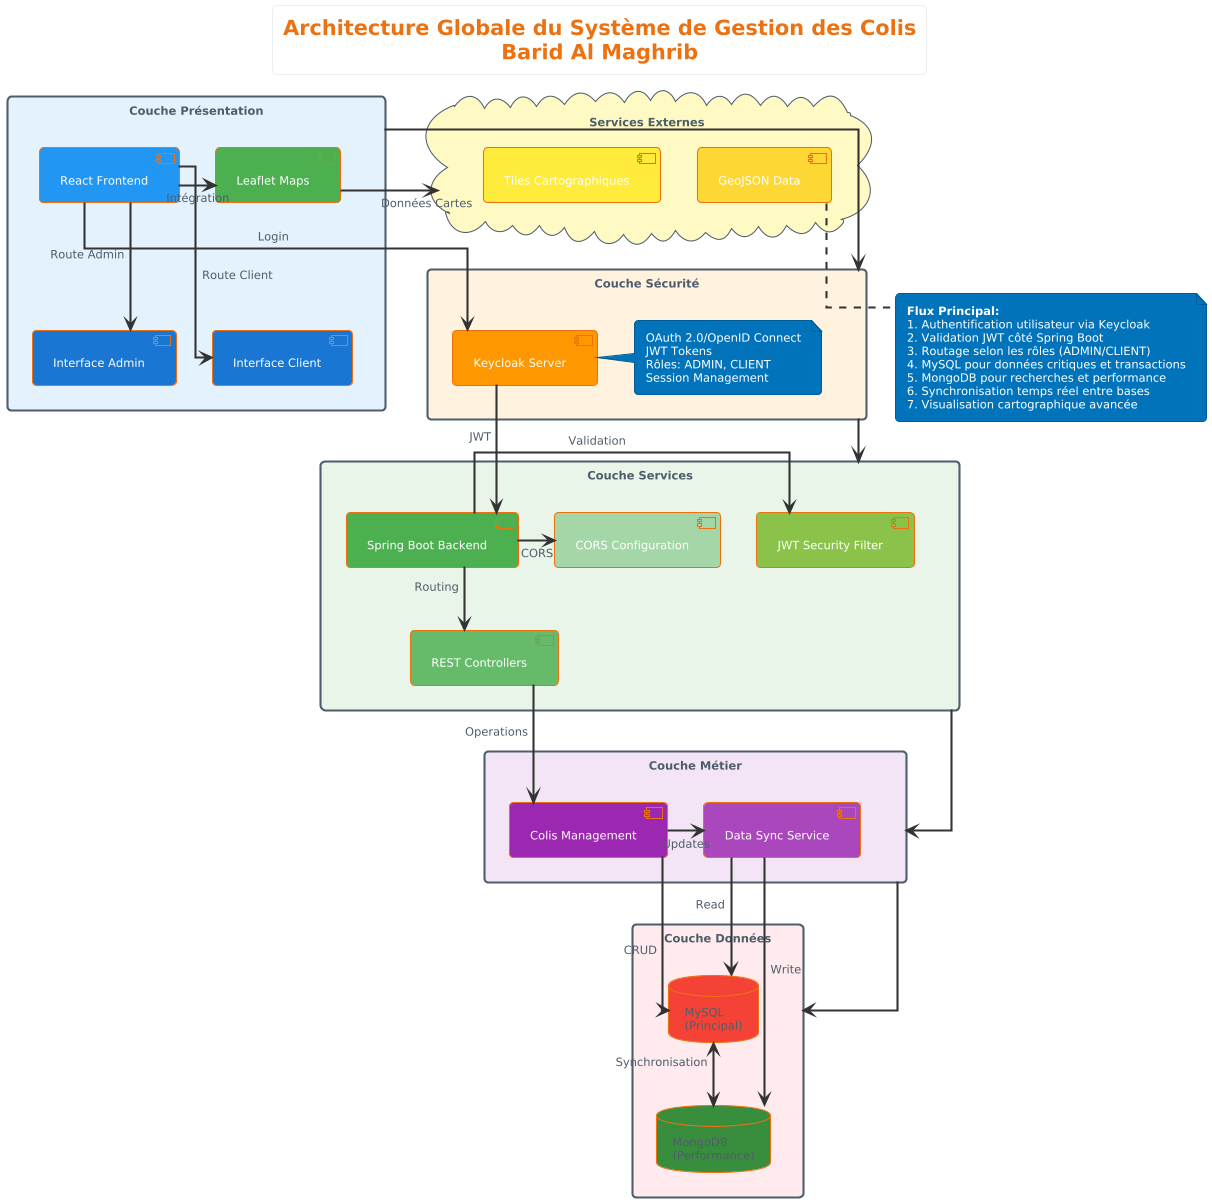
\includegraphics[width=0.8\textwidth]{images/architecture_globale.png}
\caption{Architecture globale du système hybride}
\label{fig:architecture_globale}
\end{figure}
La Figure \ref{fig:architecture_globale} présente l'architecture complète du système avec les flux de données et les interactions entre composants. La couche de présentation, développée en React, implémente une Single Page Application moderne avec gestion d'état centralisée et communication asynchrone avec les services backend via des API REST sécurisées.

La couche métier, architecturée autour de Spring Boot, expose des API REST [14] sécurisées par Keycloak et implémente la logique business complexe. Cette couche intègre le routage intelligent des requêtes vers les systèmes de persistance appropriés selon la nature des opérations : consultation rapide via MongoDB pour les listings et recherches, opérations transactionnelles via MySQL pour les modifications et la cohérence des données.

La couche de persistance hybride constitue l'innovation principale de cette architecture. MongoDB sert de cache intelligent et de moteur de recherche pour les opérations de consultation haute performance, tandis que MySQL conserve le rôle de source de vérité pour les données transactionnelles critiques. Un service de synchronisation automatique maintient la cohérence entre les deux systèmes en temps réel.

L'intégration de Keycloak [8] comme Identity and Access Management (IAM) centralise l'authentification et l'autorisation, supportant les standards OAuth 2.0 [11] et OpenID Connect [12]. Cette architecture sécurisée garantit l'isolation des données clients et la gestion fine des rôles utilisateur.

\subsection{Patterns architecturaux}

L'architecture s'appuie sur plusieurs patterns éprouvés adaptés aux spécificités du domaine postal. Le pattern Repository abstrait l'accès aux données en fournissant une interface unifiée indépendante du système de persistance sous-jacent. Cette approche facilite les tests unitaires et permet l'évolution future des choix technologiques.

Le pattern Strategy gouverne le routage des requêtes entre MySQL et MongoDB selon des critères définis : type d'opération, volume de données, exigences de cohérence. Cette stratégie s'adapte dynamiquement aux conditions d'utilisation et peut évoluer selon l'expérience opérationnelle.

Le pattern Observer est implémenté pour la synchronisation des données entre les systèmes de persistance. Les modifications effectuées sur MySQL déclenchent automatiquement la mise à jour des données correspondantes dans MongoDB, garantissant la cohérence sans impact sur les performances utilisateur.

Le pattern Facade simplifie l'interface des services complexes en exposant des API métier de haut niveau masquant la complexité technique de l'architecture hybride. Cette approche préserve la simplicité d'usage pour les développeurs frontend tout en exploitant la richesse technique du backend.

\subsection{Choix technologiques}

Les choix technologiques s'appuient sur des critères de maturité, performance, et écosystème pour garantir la pérennité de la solution. Spring Boot 3.0 constitue le framework backend principal, bénéficiant d'un écosystème riche et d'une communauté active. L'intégration native avec Spring Security facilite l'implémentation des exigences de sécurité enterprise.

MongoDB 6.0 est retenu pour la couche de cache et de recherche, exploitant ses capacités d'indexation full-text et de requêtage flexibles. Les fonctionnalités d'agrégation native permettent la génération efficace de statistiques sans impact sur les performances de consultation.

Keycloak s'impose comme solution d'authentification et d'autorisation, apportant les standards OAuth 2.0/OpenID Connect et une gestion centralisée des identités. Cette solution enterprise offre la scalabilité et les fonctionnalités avancées requises pour un opérateur de l'envergure de Barid Al Maghrib.

React 18 avec TypeScript structure le frontend moderne, exploitant les dernières innovations de performance (Concurrent Features, Suspense) et de développement productif. L'intégration de Leaflet et des librairies cartographiques spécialisées enrichit considérablement les capacités de visualisation géographique.

\section{Modélisation UML}

\subsection{Diagrammes de cas d'utilisation}

La modélisation des cas d'utilisation identifie deux acteurs principaux interagissant avec le système selon des profils d'usage distincts. L'acteur Client représente les expéditeurs utilisant les services de Barid Al Maghrib et nécessitant l'accès à leurs données d'expédition. L'acteur Administrateur dispose de privilèges étendus pour la supervision globale du système..

\begin{figure}[H]
\centering
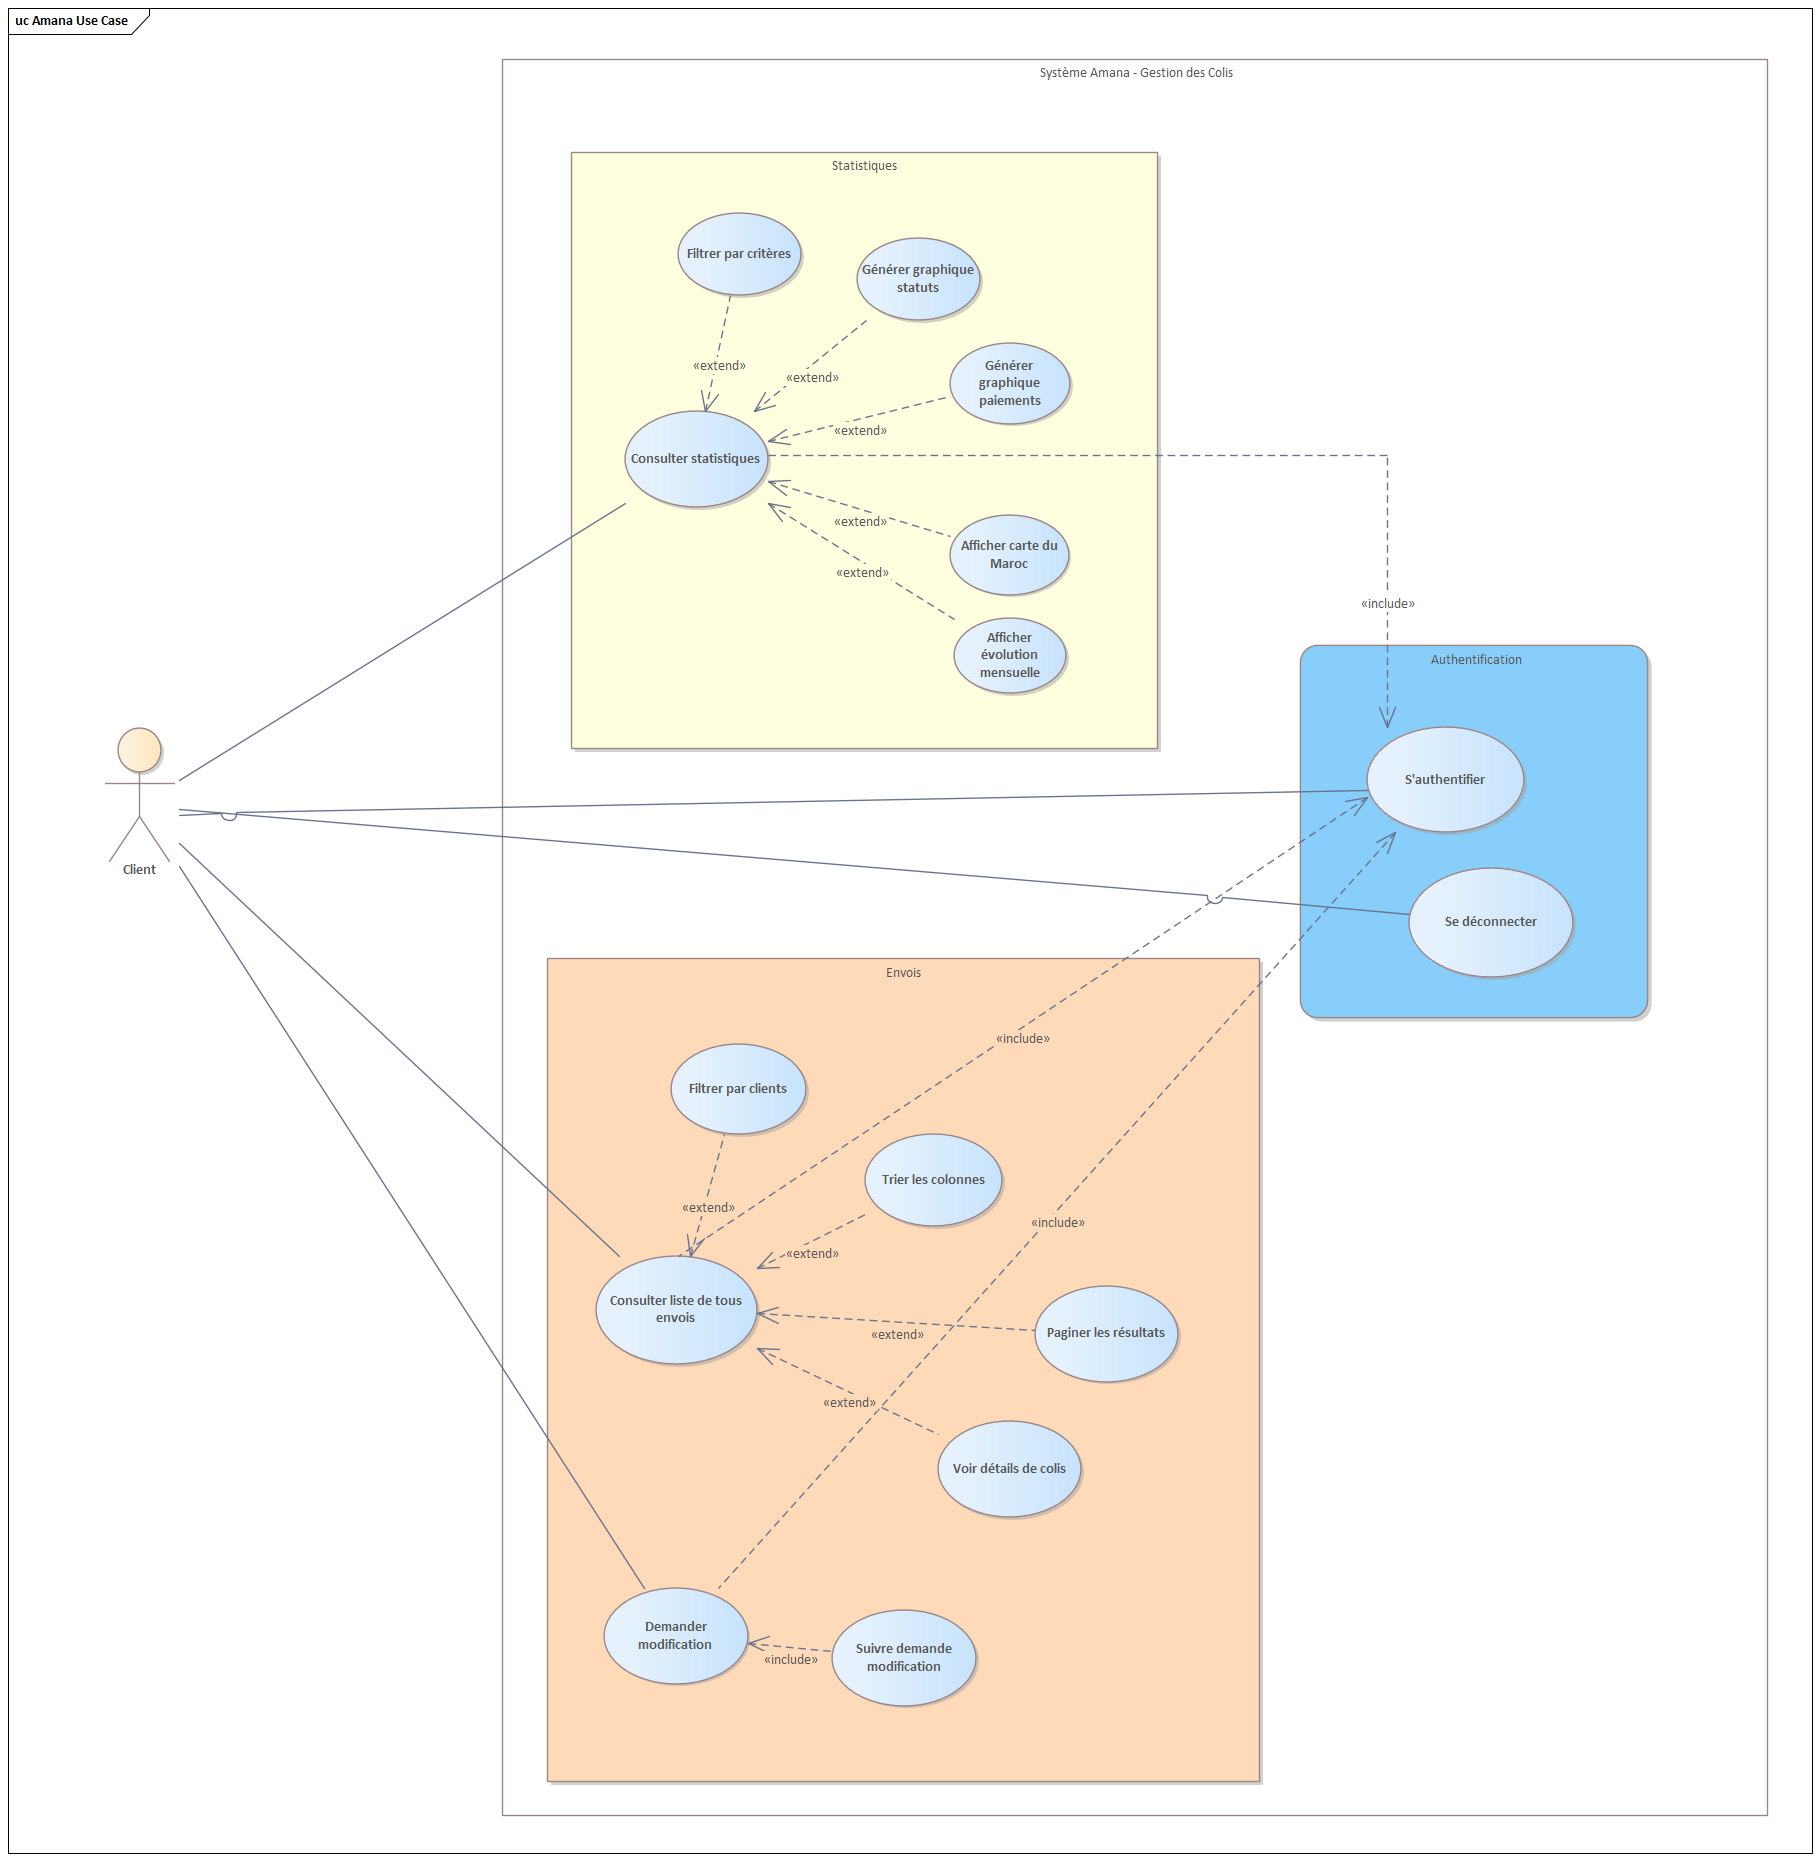
\includegraphics[width=0.8\textwidth]{images/Amana Colis Use Case Client.png}
\caption{Diagramme de cas d'utilisation - Acteur Client}
\label{fig:use_case_client}
\end{figure}

La Figure \ref{fig:use_case_client} présente les cas d'utilisation accessibles à l'acteur Client. Ce dernier peut consulter ses colis avec des capacités de filtrage et de recherche avancées, accéder aux détails individuels de chaque envoi, soumettre des demandes de modification pour les informations non critiques, et générer des statistiques personnalisées de son activité d'expédition.

\begin{figure}[H]
\centering
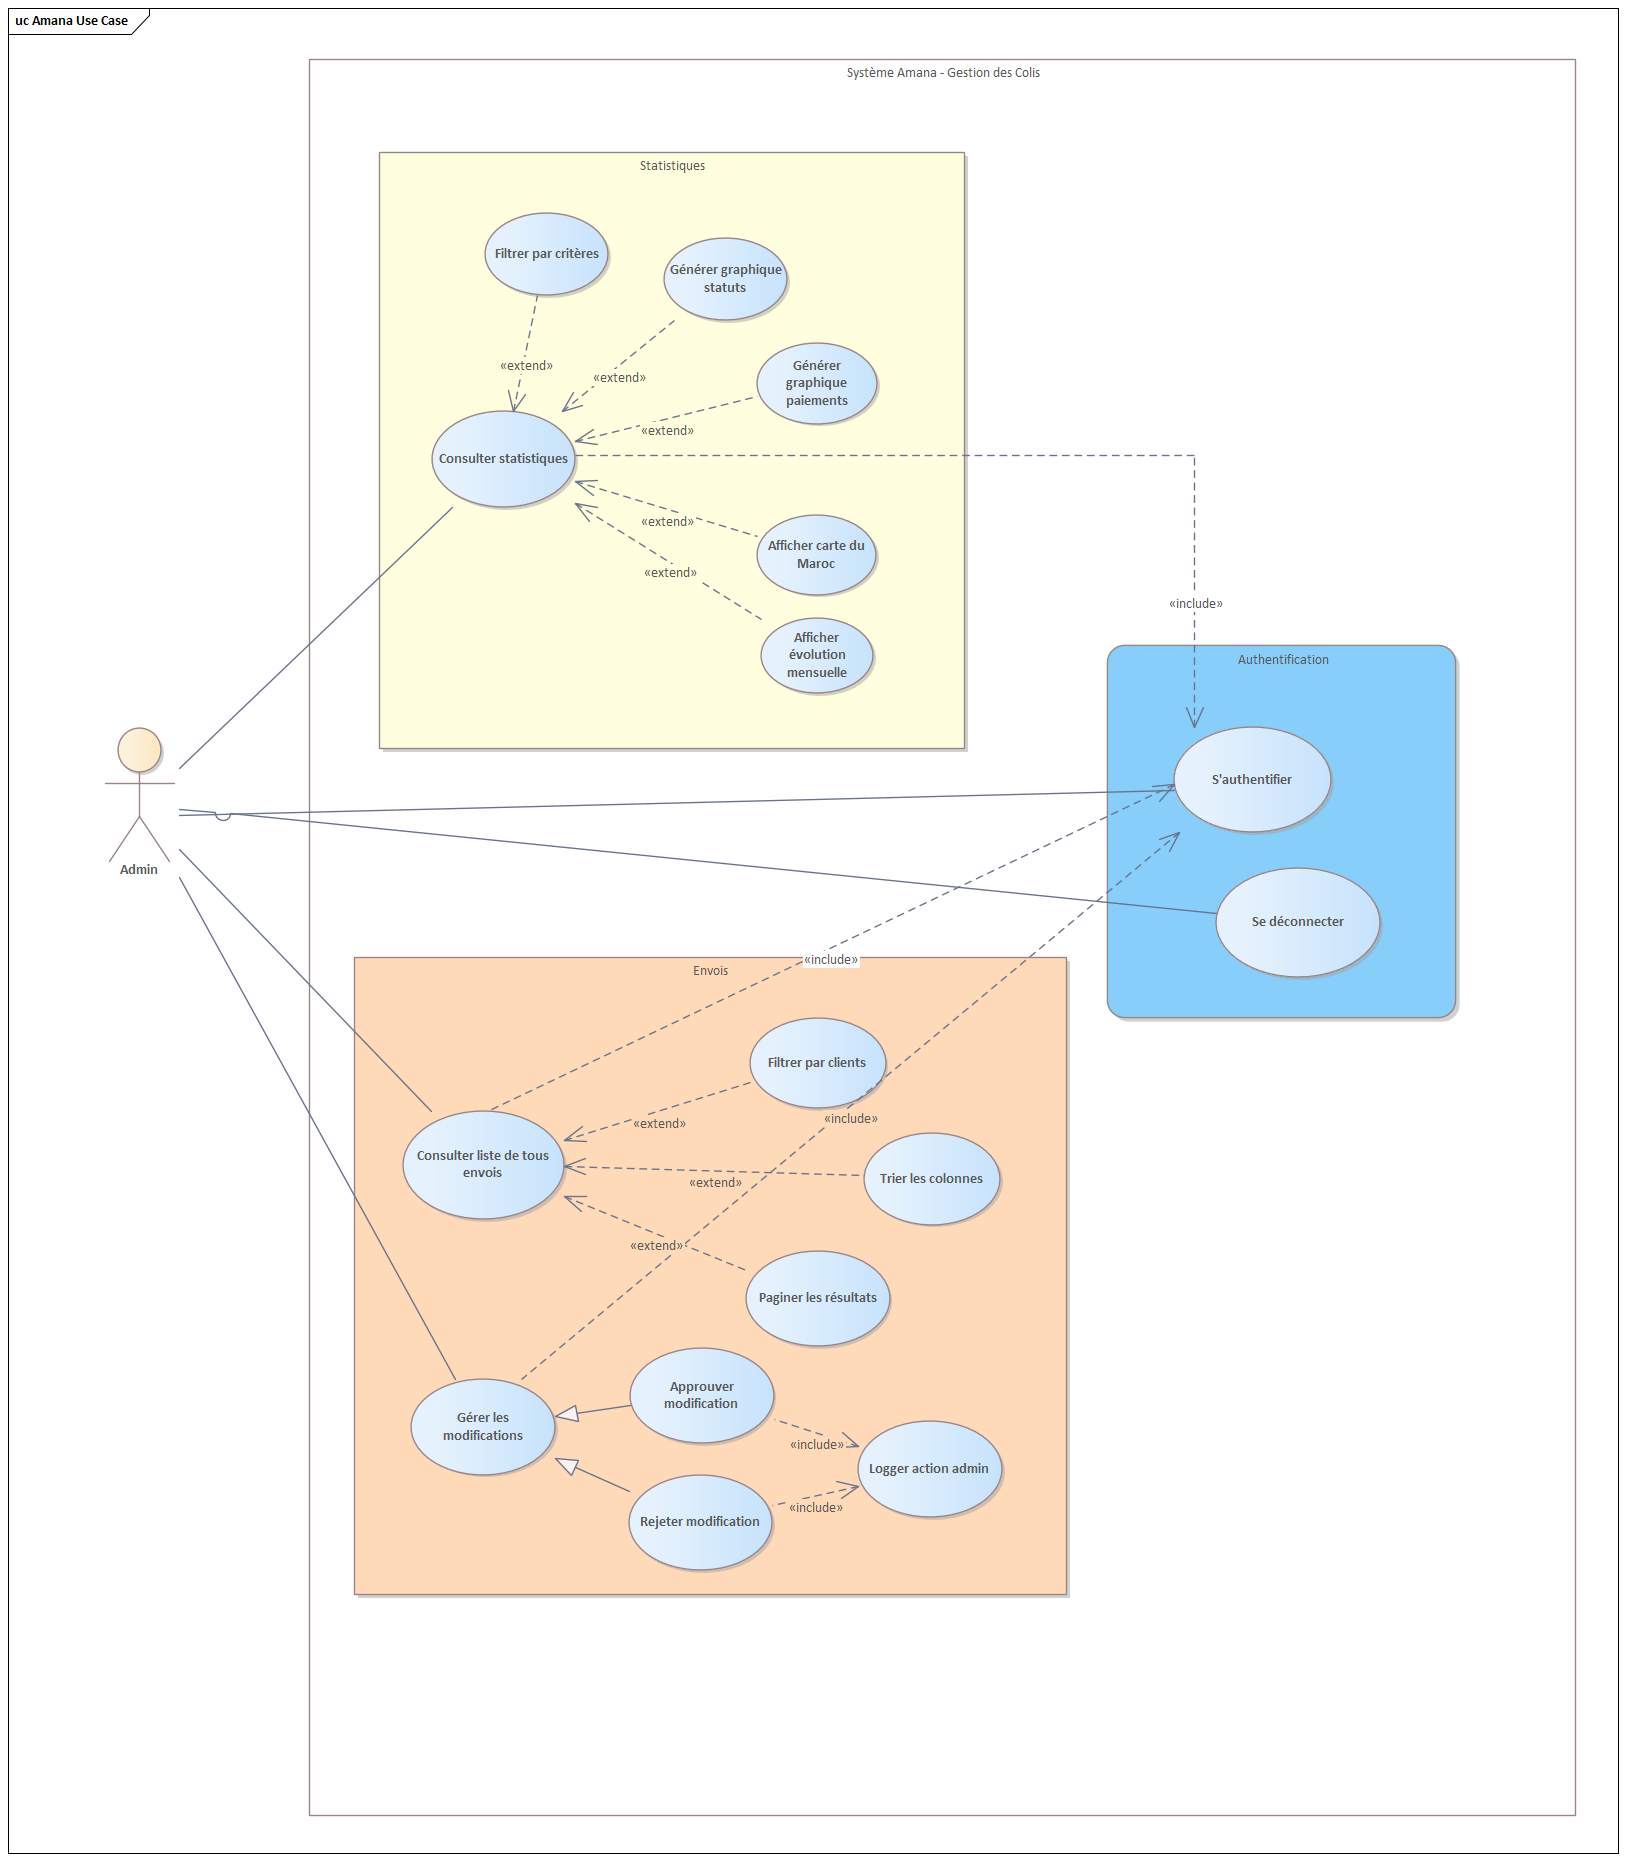
\includegraphics[width=0.8\textwidth]{images/Amana Colis Use Case Admin.png}
\caption{Diagramme de cas d'utilisation - Acteur Administrateur}
\label{fig:use_case_admin}
\end{figure}

La Figure \ref{fig:use_case_admin} détaille les privilèges étendus de l'acteur Administrateur. Il dispose d'un accès global à l'ensemble des données colis tous clients confondus, peut valider ou rejeter les demandes de modification avec traçabilité complète.

\subsection{Diagrammes de séquence}

Le diagramme de séquence de consultation des colis illustre l'orchestration complexe entre les différents composants du système hybride, mettant en évidence l'intégration de Keycloak pour l'authentification et le routage intelligent vers MongoDB pour l'optimisation des performances.

\begin{figure}[H]
\centering
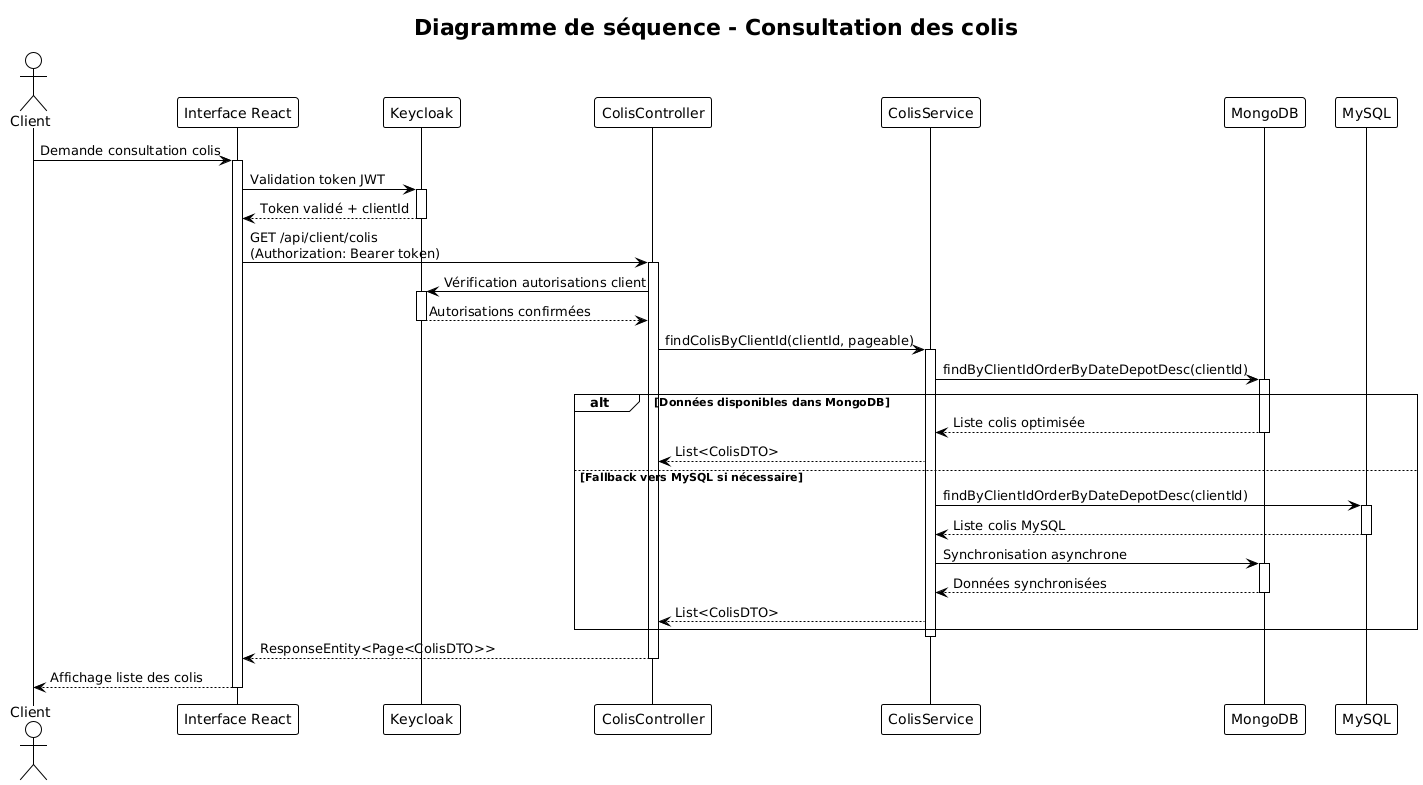
\includegraphics[width=1.0\textwidth]{images/sequence_consultation.png}
\caption{Diagramme de séquence - Consultation des colis}
\label{fig:sequence_consultation}
\end{figure}
La Figure \ref{fig:sequence_consultation} montre l'interaction complète depuis l'authentification utilisateur jusqu'à l'affichage des données. Le processus débute par la validation du token JWT via Keycloak, suivi de la vérification des autorisations client. La requête est ensuite routée vers MongoDB pour récupération optimisée des données de listing, avec fallback vers MySQL si nécessaire.

\begin{figure}[H]
\centering
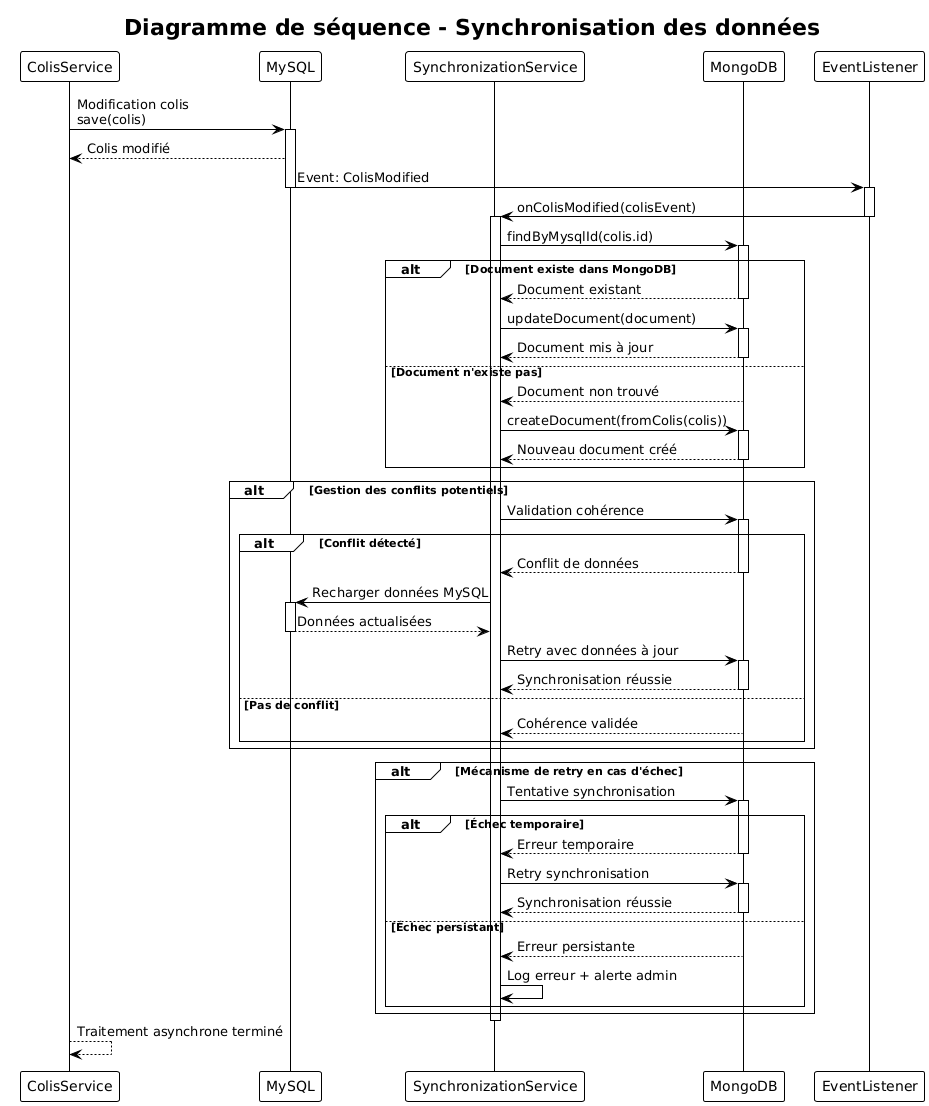
\includegraphics[width=0.9\textwidth]{images/sequence_synchronisation.png}
\caption{Diagramme de séquence - Synchronisation des données}
\label{fig:sequence_synchronisation}
\end{figure}
La Figure \ref{fig:sequence_synchronisation} modélise le processus critique de maintien de cohérence entre MySQL et MongoDB. Toute modification sur MySQL déclenche un événement traité asynchronement par le service de synchronisation, qui met à jour les documents correspondants dans MongoDB avec gestion des conflits potentiels et mécanismes de retry en cas d'échec.

\subsection{Diagrammes de classes}

La modélisation objet identifie les entités métier principales et leurs relations, ainsi que les classes techniques nécessaires à l'implémentation de l'architecture hybride.

\begin{figure}[H]
\centering
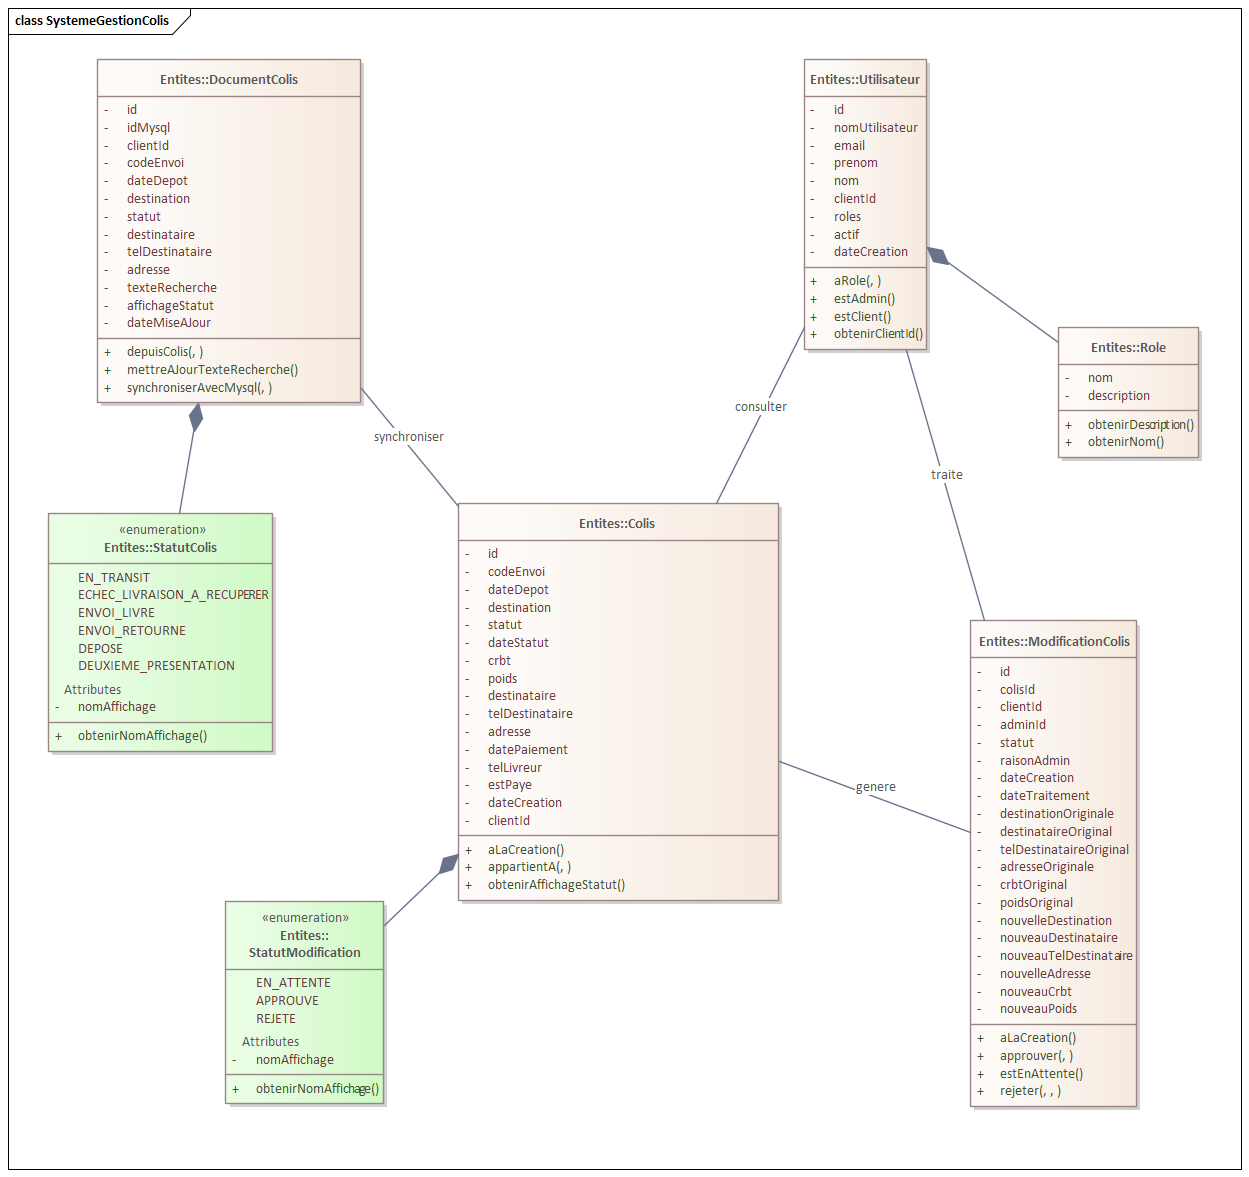
\includegraphics[width=1.1\textwidth]{images/class_diagram.png}
\caption{Diagramme de classes principal}
\label{fig:class_diagram}
\end{figure}

La Figure \ref{fig:class_diagram} présente la structure objet du système avec les entités métier centrales. La classe \texttt{Colis} constitue l'entité principale encapsulant l'ensemble des informations descriptives. La classe \texttt{Utilisateur} modélise les expéditeurs avec ses attributions d'identification et autorisations d'accès. La classe \texttt{ColisModification} gère le workflow d'approbation des demandes de changement.
\newpage
\subsection{Modèle de données}

Le modèle de données hybride concilie les paradigmes relationnels et documentaires pour optimiser les différents patterns d'accès selon les besoins fonctionnels identifiés.

\begin{figure}[H]
\centering
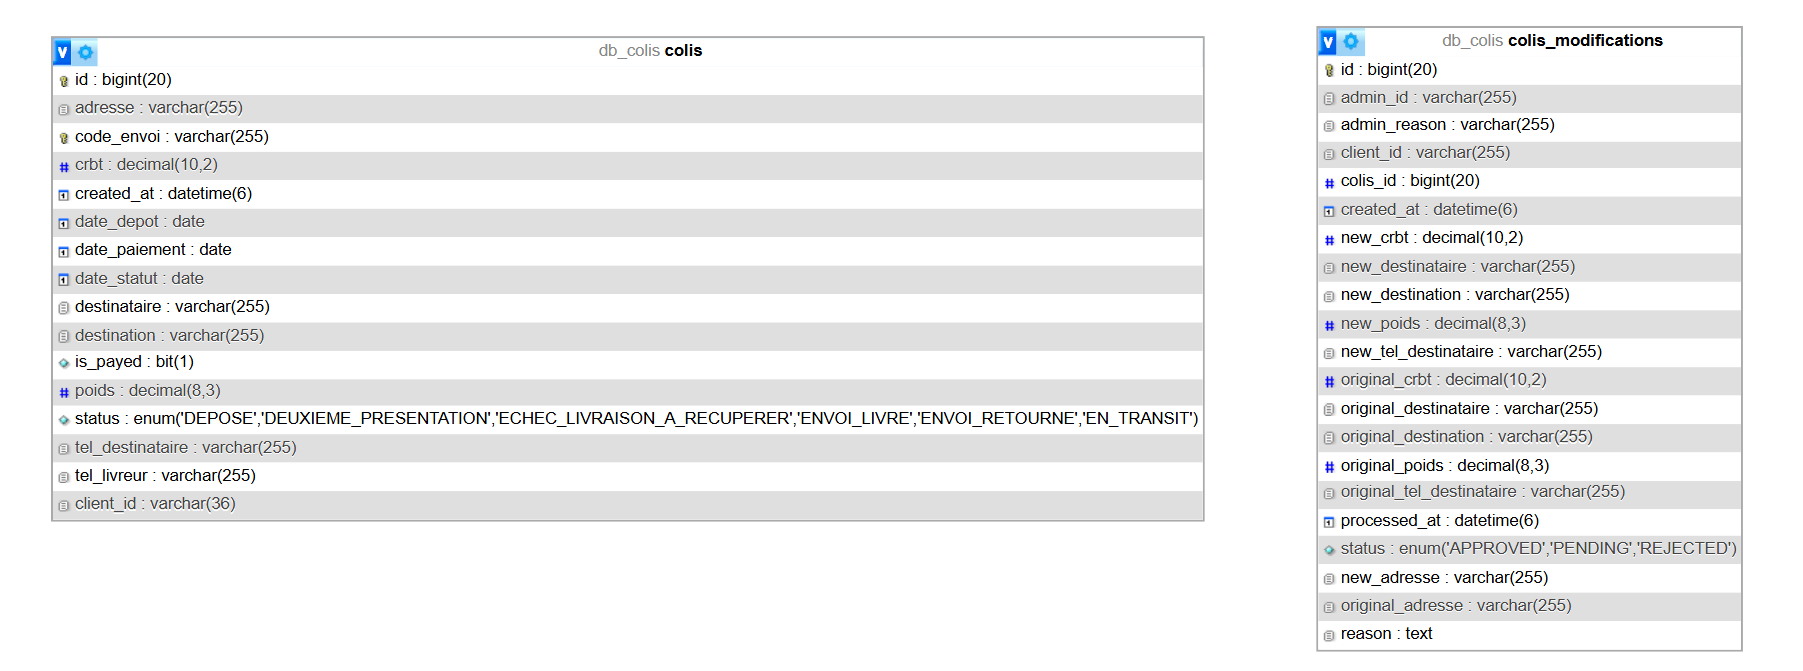
\includegraphics[width=1.0\textwidth]{images/data_model_mysql.png}
\caption{Modèle de données MySQL}
\label{fig:data_model_mysql}
\end{figure}
La Figure \ref{fig:data_model_mysql} illustre la structure relationnelle MySQL avec les tables principales et leurs relations. Le modèle normalisé garantit l'intégrité transactionnelle avec les contraintes d'intégrité référentielle appropriées. Les index composites optimisent les requêtes fréquentes tout en préservant les performances des opérations transactionnelles.

\section{Conception de la Base de Données}

\subsection{Modèle relationnel (MySQL)}

Le modèle relationnel MySQL préserve la structure normalisée garantissant l'intégrité transactionnelle et la cohérence des données critiques pour les opérations de Barid Al Maghrib.

\begin{figure}[H]
\centering
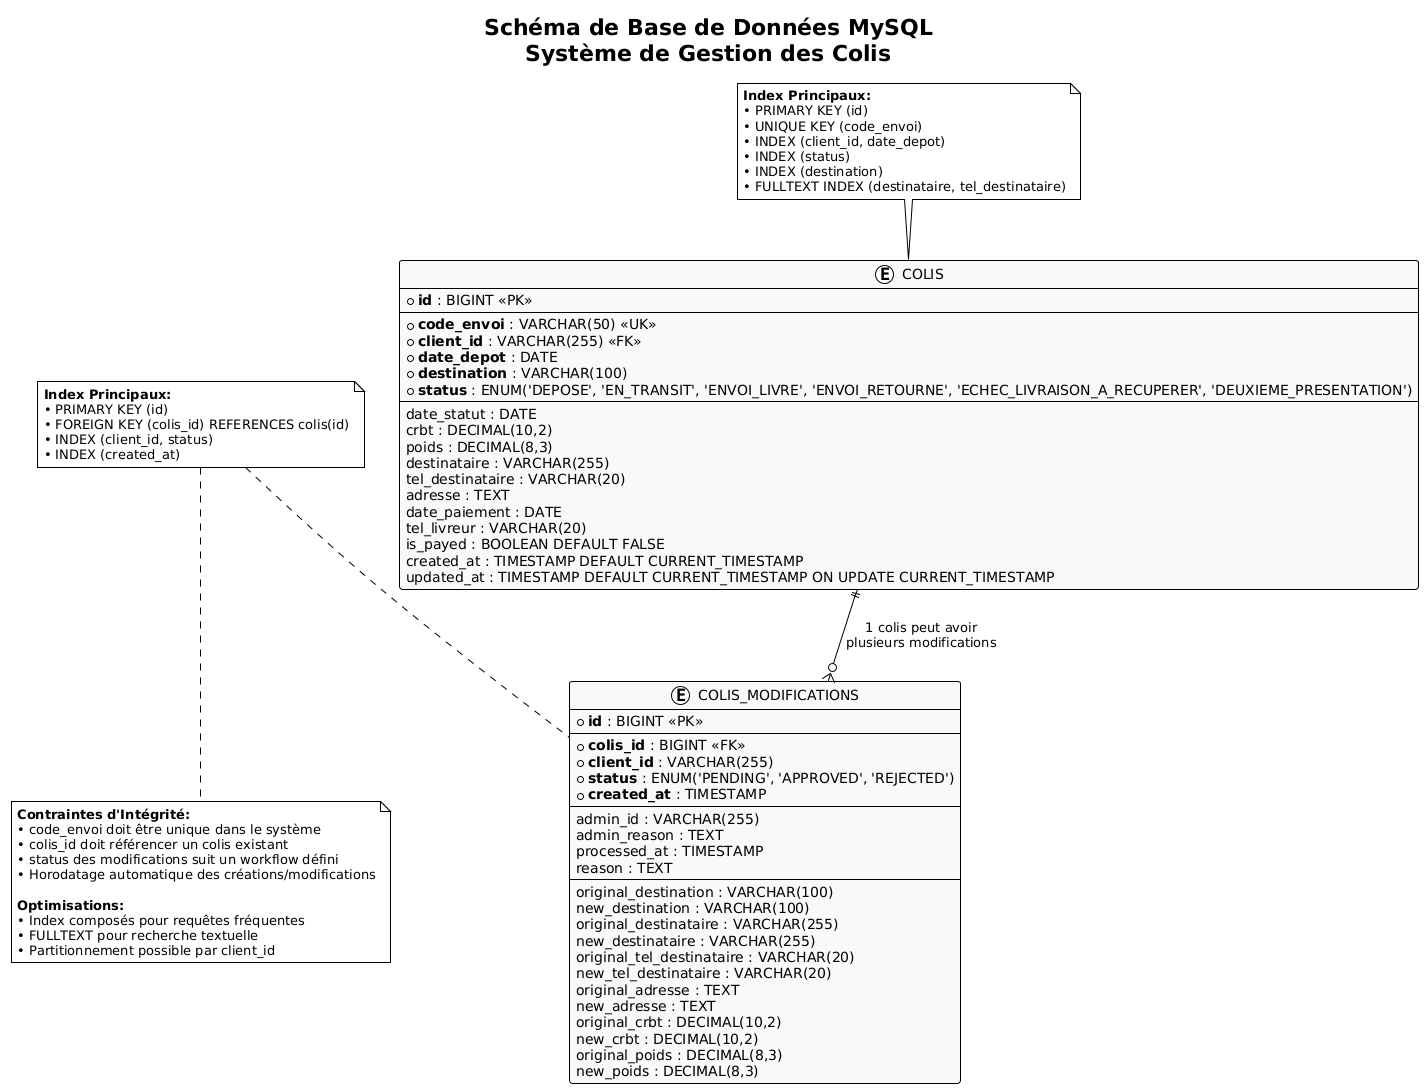
\includegraphics[width=1.0\textwidth]{images/mysql_schema.png}
\caption{Schéma de base de données MySQL}
\label{fig:mysql_schema}
\end{figure}

La Figure \ref{fig:mysql_schema} présente la structure détaillée de la base MySQL avec les contraintes d'intégrité référentielle. La table \texttt{colis} constitue l'entité principale avec ses attributs obligatoires : \texttt{id}, \texttt{code\_envoi}, \texttt{client\_id}, \texttt{date\_depot}, \texttt{destination}, \texttt{status}. La table \texttt{colis\_modifications} modélise le workflow d'approbation des changements avec conservation de l'historique complet.

L'optimisation des performances MySQL s'appuie sur une stratégie d'indexation ciblée : index composites sur \texttt{(client\_id, date\_depot)} pour les consultations client, index sur \texttt{status} et \texttt{destination} pour les filtres administrateur, index full-text sur les champs de recherche textuelle.

\subsection{Modèle NoSQL (MongoDB)}

Le modèle documentaire MongoDB privilégie la dénormalisation pour optimiser les performances de lecture et simplifier les requêtes de consultation utilisateur quotidiennes.

\begin{figure}[H]
\centering
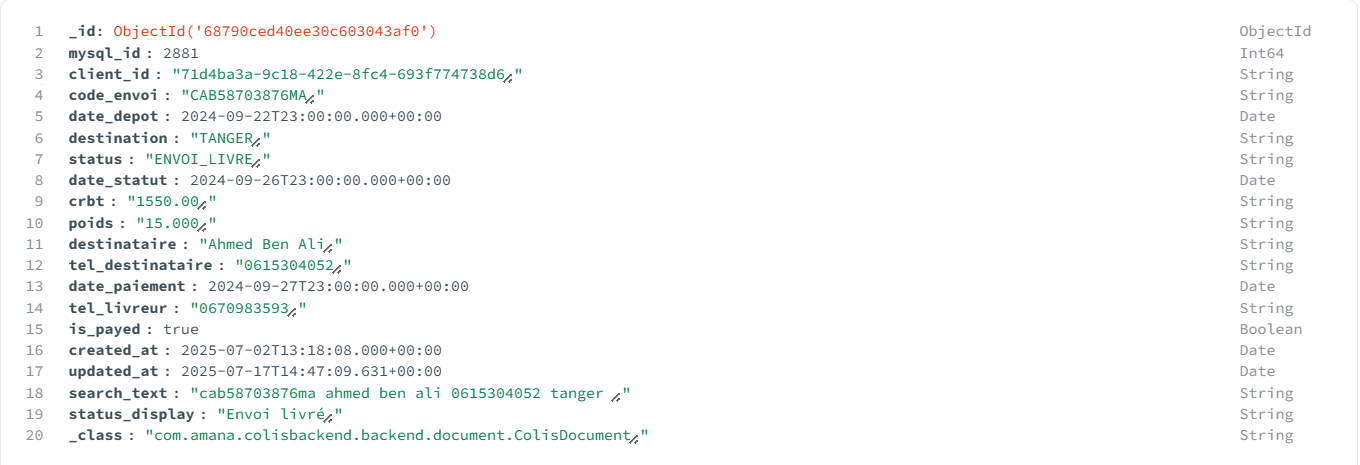
\includegraphics[width=1.3\textwidth]{images/mongodb_document.png}
\caption{Structure des documents MongoDB}
\label{fig:mongodb_document}
\end{figure}

La Figure \ref{fig:mongodb_document} illustre la structure documentaire optimisée avec les champs calculés et les index spécialisés. Les documents intègrent l'ensemble des informations nécessaires aux vues listing, éliminant les jointures coûteuses. La stratégie d'indexation exploite les spécificités NoSQL : index composés sur \texttt{(clientId, dateDepot)}, index text sur \texttt{search\_text}, index géospatiaux pour les requêtes cartographiques.


% Partie 4 : Réalisation et Développement
\chapter{Réalisation et Développement}

\section{Environnement de Développement}

\subsection{Outils et IDE}

L'environnement de développement a été soigneusement configuré pour maximiser la productivité et garantir la qualité du code produit. 

\begin{figure}[H]
\centering
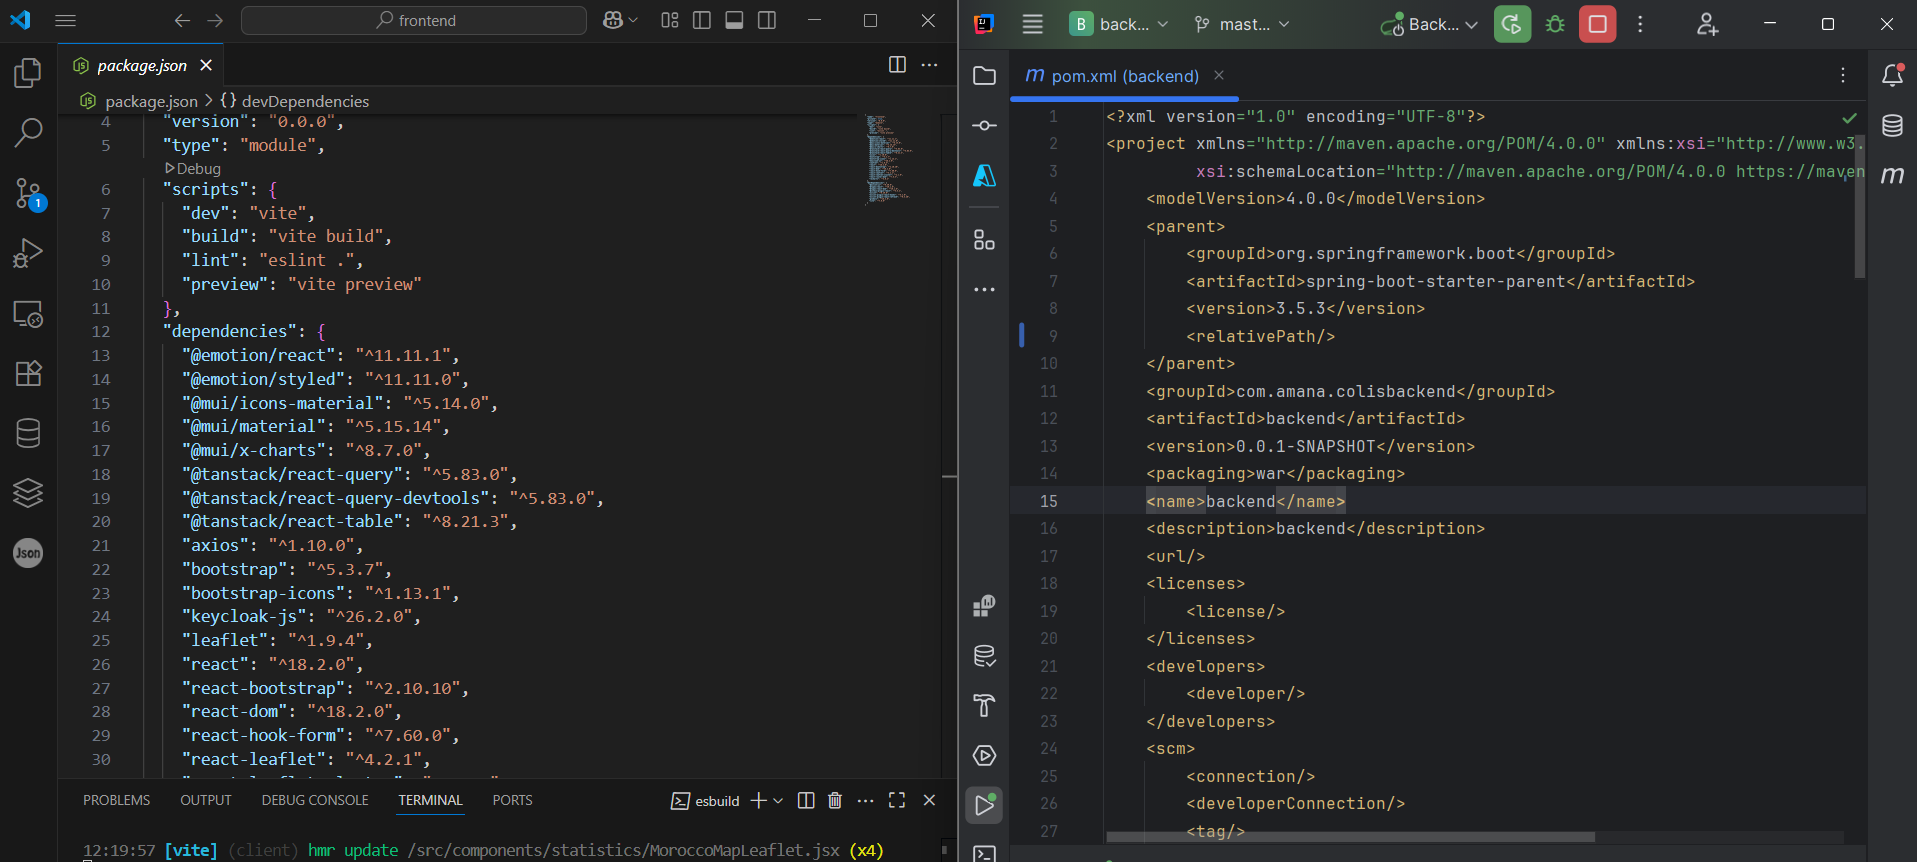
\includegraphics[width=1.0\textwidth]{images/dev_environment.png}
\caption{Environnement de développement complet}
\label{fig:dev_environment}
\end{figure}

La Figure \ref{fig:dev_environment} présente l'environnement de développement utilisé avec IntelliJ IDEA Ultimate pour le backend Spring Boot et Visual Studio Code pour le frontend React. IntelliJ IDEA [15] offre une intégration native excellente avec les frameworks Spring, des outils de débogage avancés, et un support complet de MongoDB. Visual Studio Code [16] a été choisi pour sa richesse d'extensions React et sa légèreté pour le développement frontend.

Git [17] a été configuré avec des hooks de pre-commit pour automatiser la vérification de la qualité du code. Docker [18] facilite la gestion des services externes (MongoDB, MySQL, Keycloak) avec des configurations prêtes à l'emploi, assurant la reproductibilité de l'environnement entre les différents postes de développement.

\subsection{Frameworks et bibliothèques}

\begin{figure}[H]
\centering
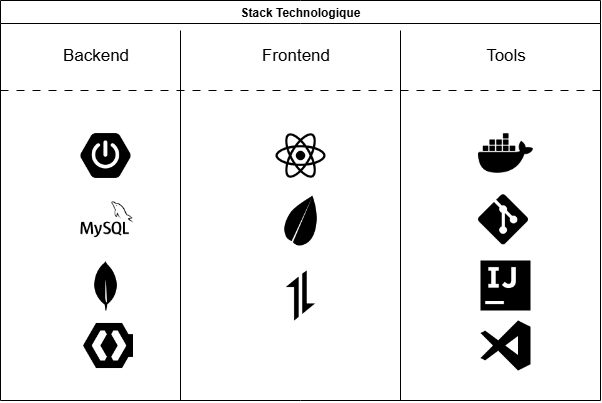
\includegraphics[width=0.8\textwidth]{images/tech_stack.png}
\caption{Stack technologique utilisée}
\label{fig:tech_stack}
\end{figure}

La Figure \ref{fig:tech_stack} illustre la stack technologique complète du projet. Le backend s'articule autour de Spring Boot 3.1 [1] avec Spring Data JPA [3] pour MySQL et Spring Data MongoDB [4] pour la base documentaire. Spring Security 6.1 [2] gère l'authentification OAuth2 [11,12] avec Keycloak [8]. Le frontend React 18.2 [5] exploite les dernières fonctionnalités de performance avec React Router [22] pour la navigation et Axios [21] pour les communications HTTP.

La cartographie utilise Leaflet [9] avec React-Leaflet [10], enrichie par Leaflet.markercluster [24] pour le clustering des points et des providers de tiles haute résolution. Cette combinaison offre des performances d'affichage optimales même avec des milliers de marqueurs simultanés.

\subsection{Configuration du projet}

\begin{figure}[H]
\centering
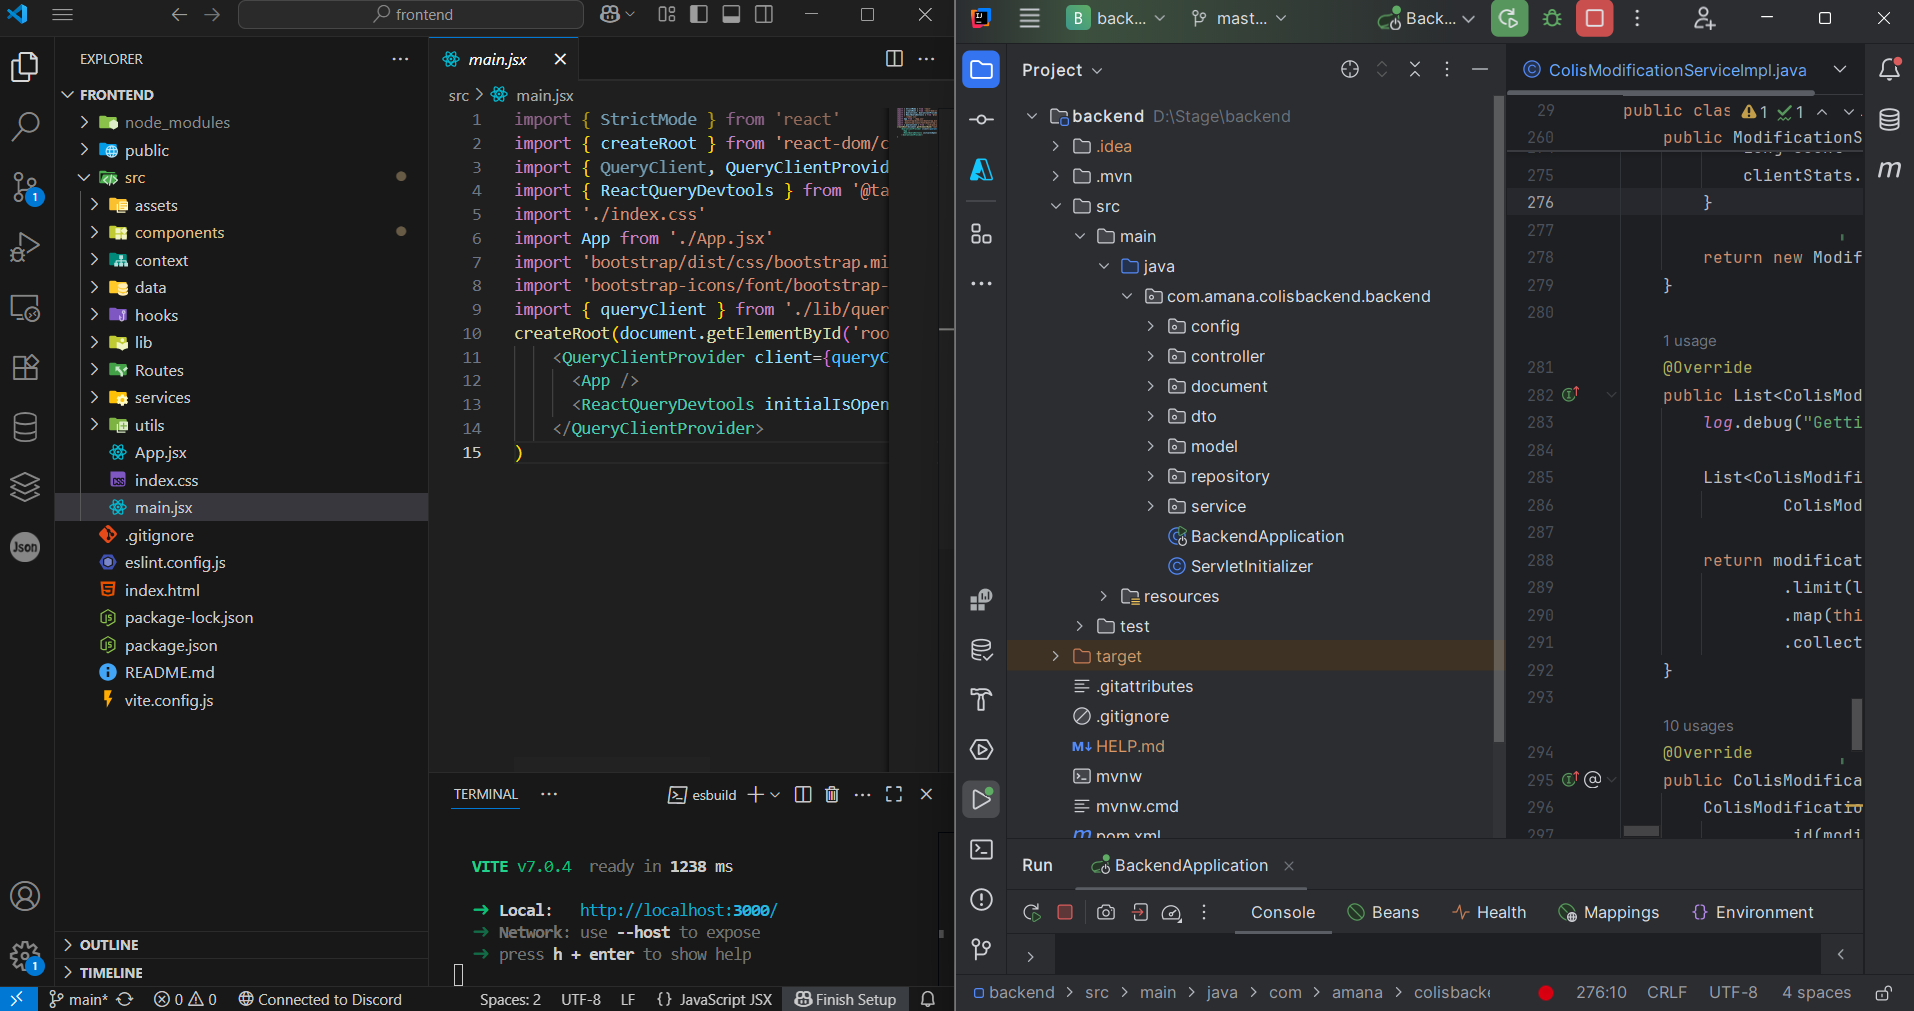
\includegraphics[width=0.8\textwidth]{images/project_structure.png}
\caption{Structure du projet et organisation des fichiers}
\label{fig:project_structure}
\end{figure}

La Figure \ref{fig:project_structure} montre l'organisation du projet respectant les bonnes pratiques d'architecture. Le backend adopte une organisation par feature plutôt que par couche technique, facilitant la maintenance. Le frontend suit la structure Create React App avec des dossiers organisés par fonctionnalité : components, services, hooks, utils.

\section{Développement Backend}

\subsection{Architecture Spring Boot}

\begin{figure}[H]
\centering
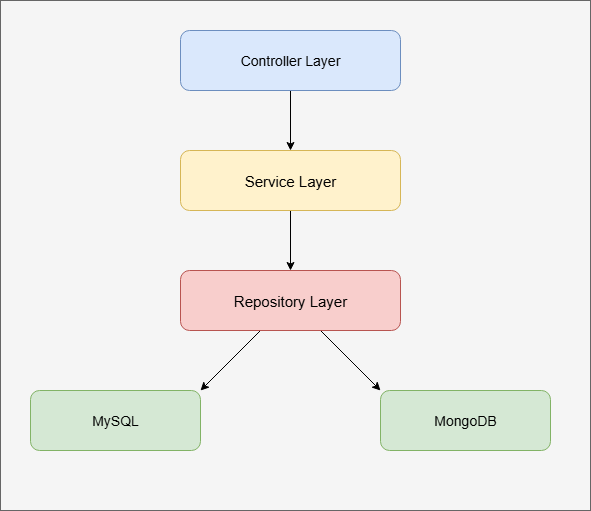
\includegraphics[width=0.5\textwidth]{images/spring_architecture.png}
\caption{Architecture Spring Boot avec couches séparées}
\label{fig:spring_architecture}
\end{figure}

La Figure \ref{fig:spring_architecture} illustre l'architecture backend implémentant le pattern Repository avec une couche de service métier orchestrant les interactions entre MySQL et MongoDB. La couche Controller expose les API REST, la couche Service implémente la logique métier, et la couche Repository abstrait l'accès aux données avec des implémentations spécialisées.

\subsection{Services et contrôleurs}

\begin{figure}[H]
\centering
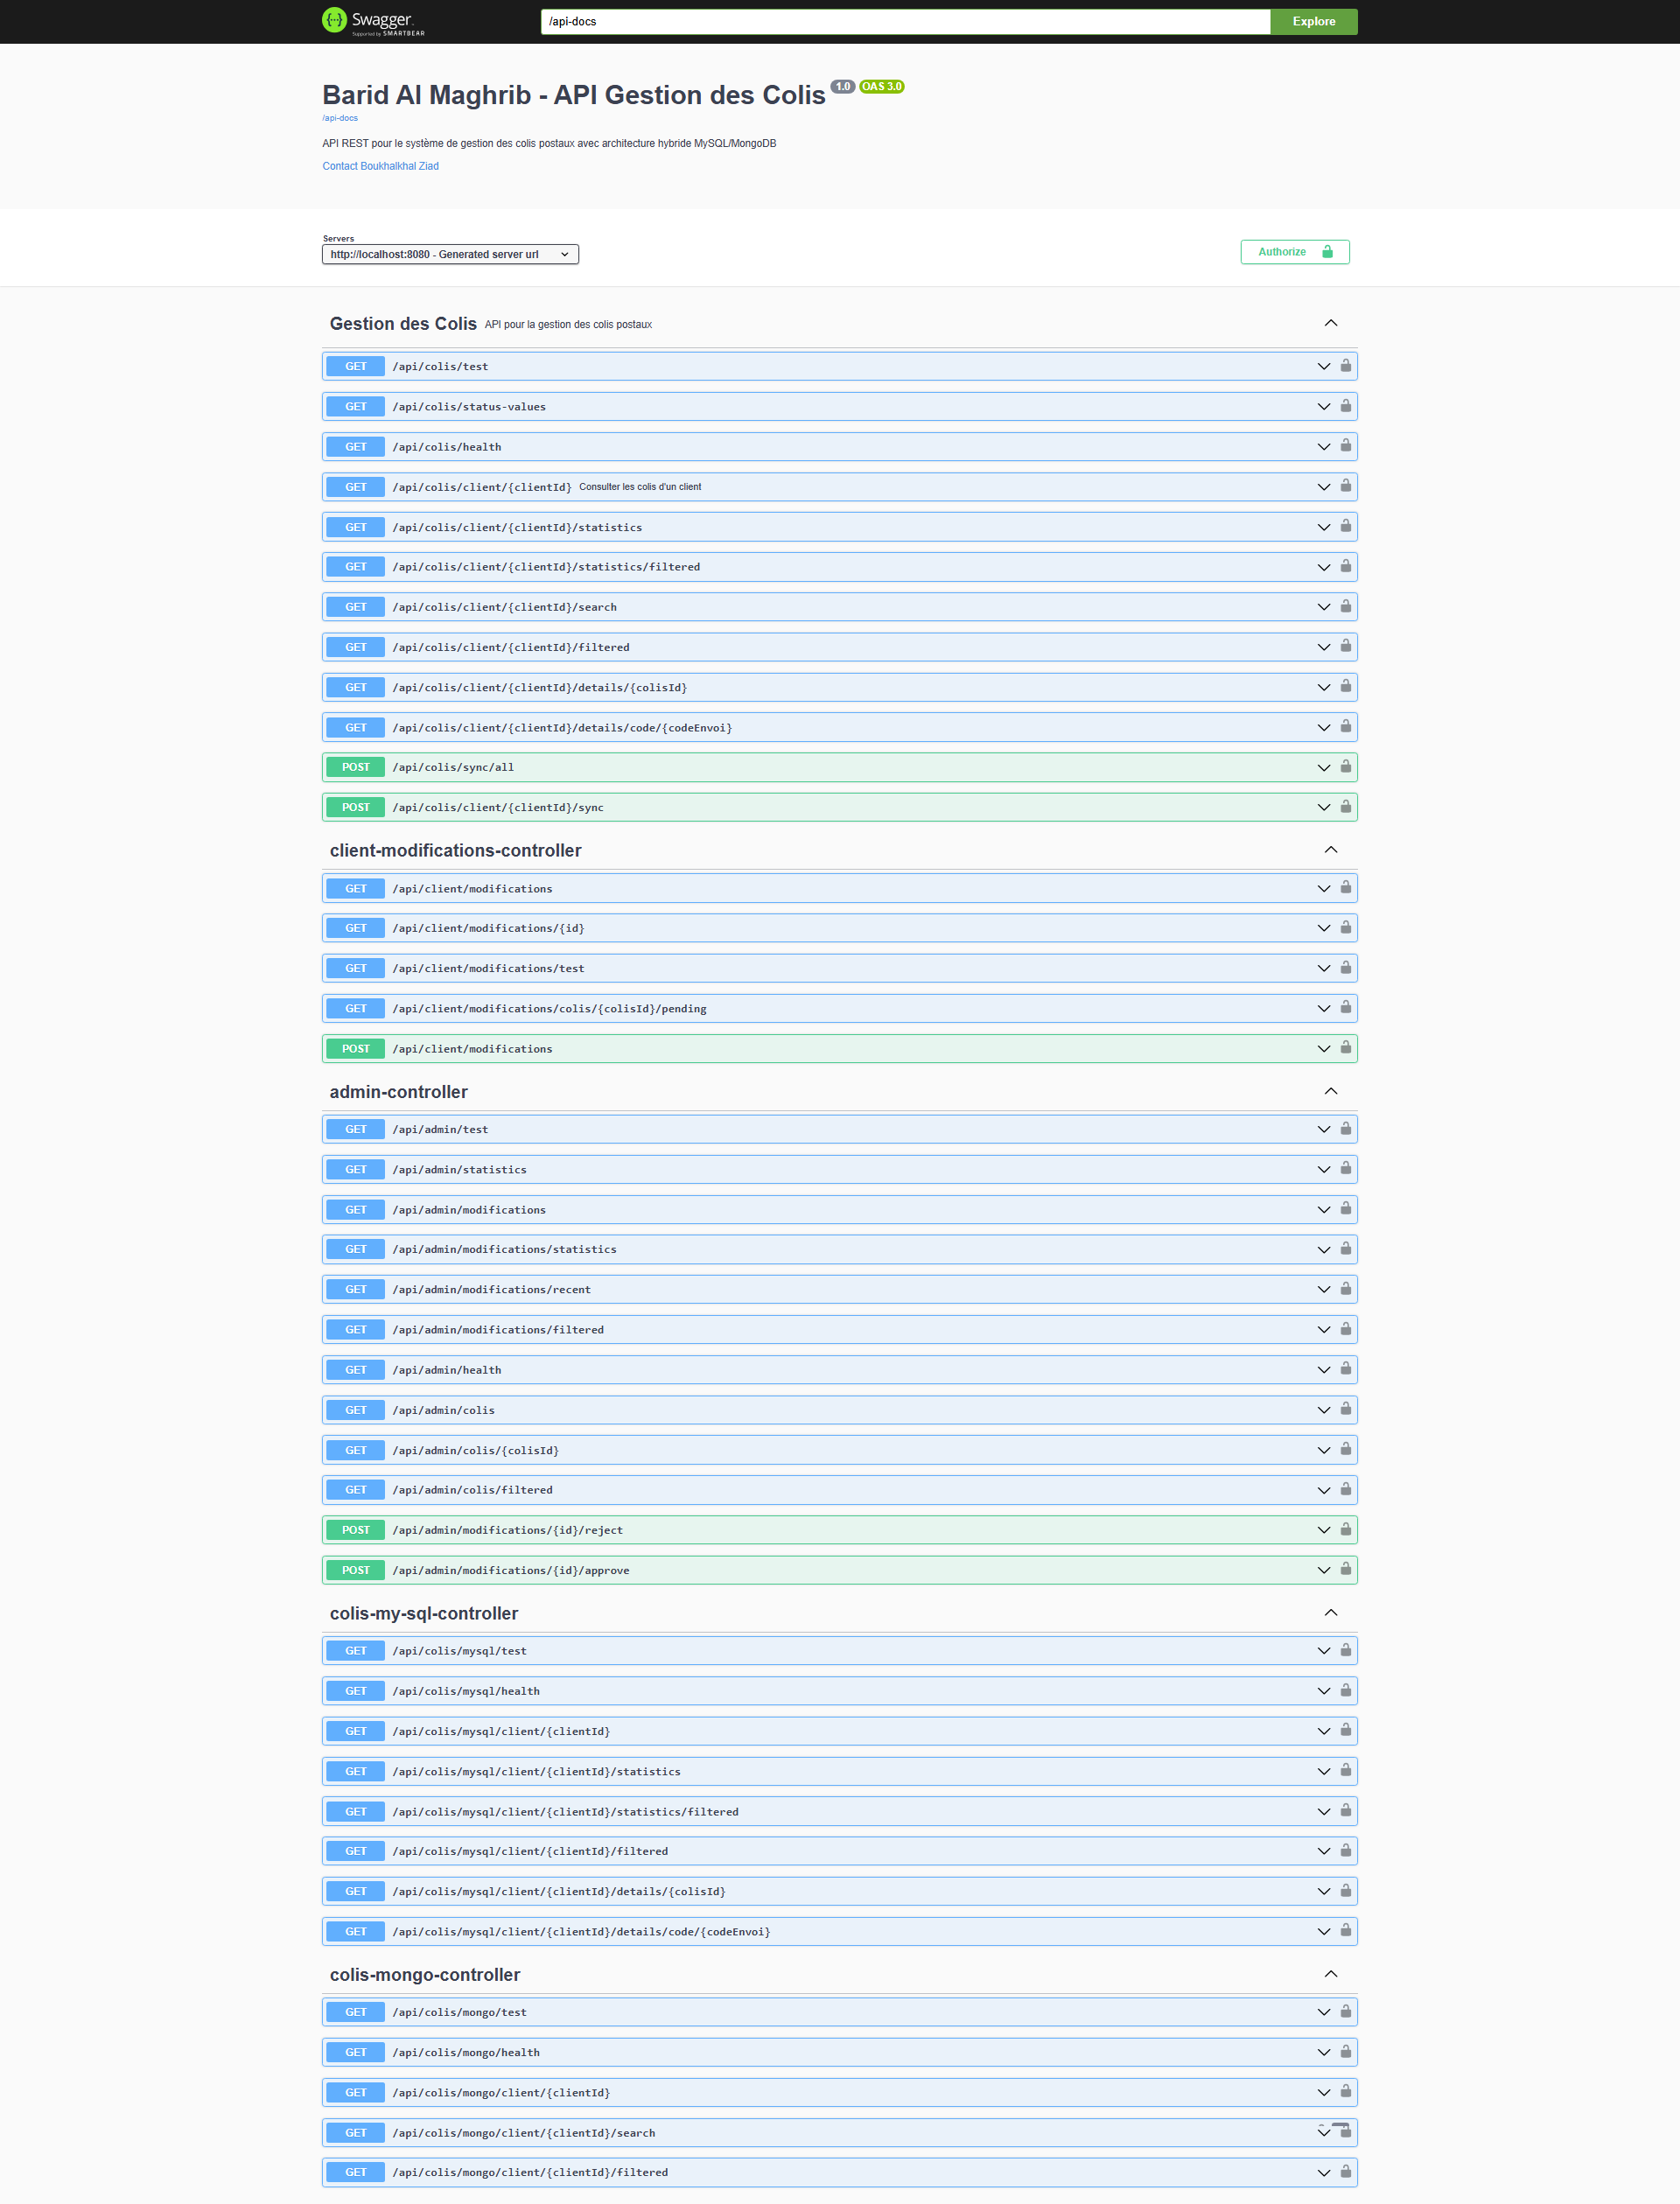
\includegraphics[width=0.7\textwidth]{images/api_endpoints.png}
\caption{Documentation des endpoints API REST}
\label{fig:api_endpoints}
\end{figure}

La Figure \ref{fig:api_endpoints} présente la documentation automatique des API REST générée par OpenAPI/Swagger. Les endpoints respectent les principes RESTful avec validation automatique des autorisations via l'extraction du \texttt{client\_id} depuis le token JWT. Chaque endpoint inclut la gestion d'erreurs appropriée et les codes de statut HTTP standards.

\subsection{Couche d'accès aux données}

L'implémentation du pattern Repository s'appuie sur Spring Data JPA pour MySQL et Spring Data MongoDB pour la base documentaire. Cette dualité nécessite une abstraction soignée pour masquer la complexité aux couches supérieures tout en exploitant les spécificités de chaque technologie.

\subsection{API REST}

\begin{figure}[H]
\centering
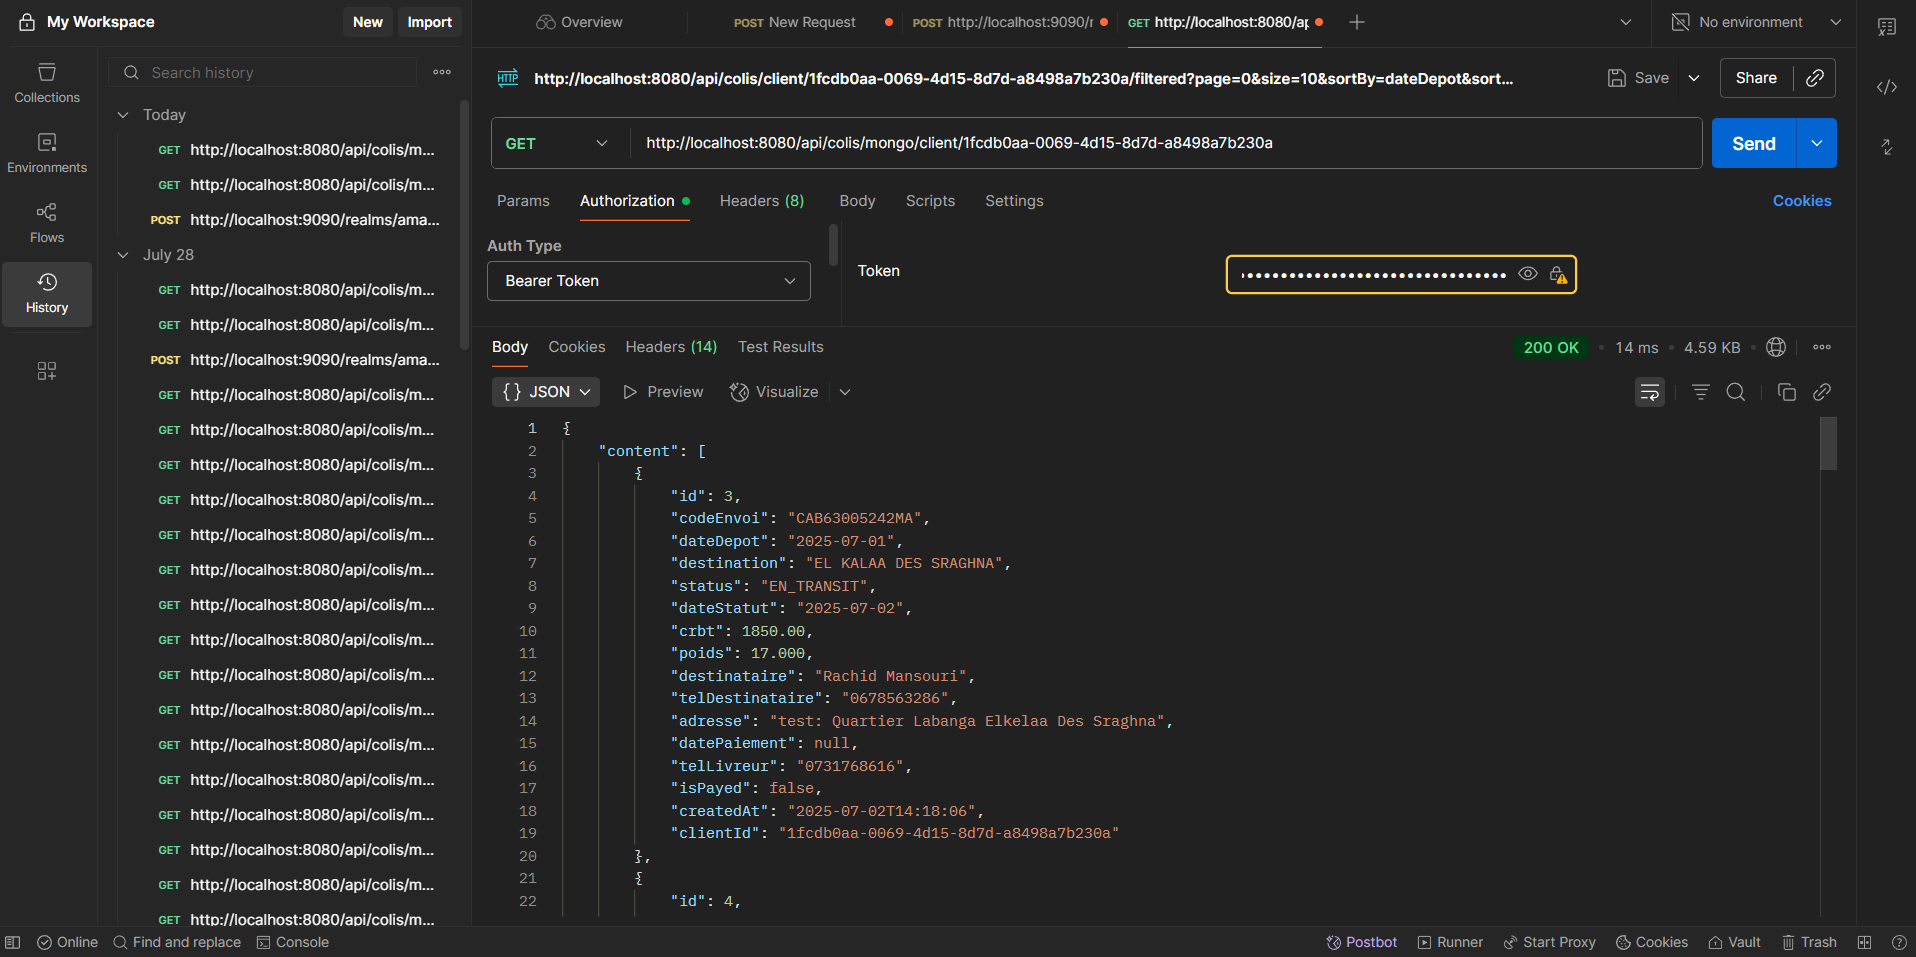
\includegraphics[width=1.0\textwidth]{images/postman_tests.png}
\caption{Tests des API avec Postman}
\label{fig:postman_tests}
\end{figure}

La Figure \ref{fig:postman_tests} montre les tests des API REST avec Postman [19], incluant la validation des tokens JWT [13], les tests de performance, et la vérification des autorisations. Cette approche garantit la robustesse et la sécurité des endpoints avant leur utilisation par le frontend.

\subsection{Sécurité avec Keycloak}

\begin{figure}[H]
\centering
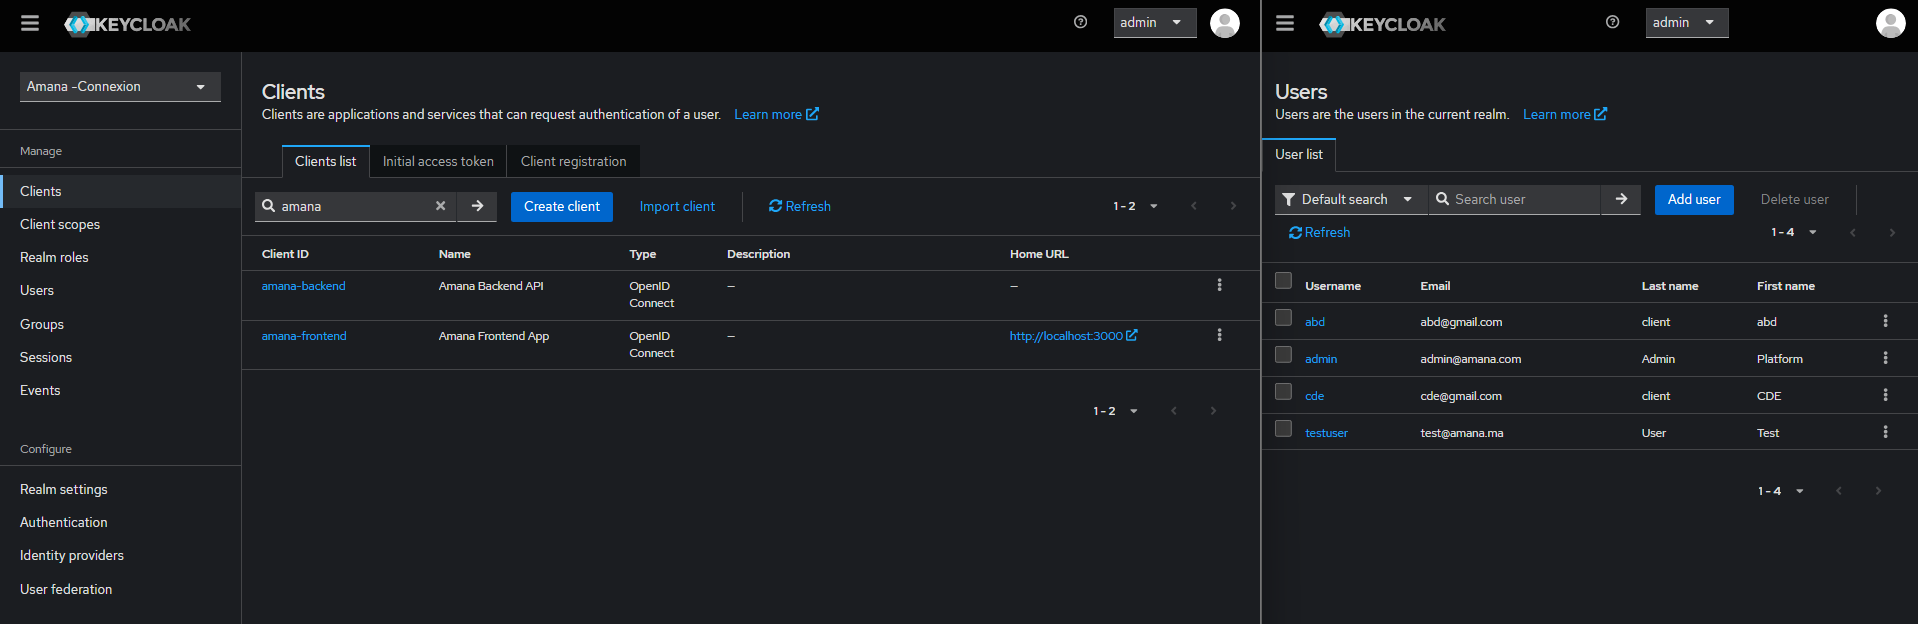
\includegraphics[width=1.0\textwidth]{images/keycloak_config.png}
\caption{Configuration Keycloak - Realm et clients}
\label{fig:keycloak_config}
\end{figure}

La Figure \ref{fig:keycloak_config} présente la configuration Keycloak avec le realm "amana-realm" et ses clients (backend et frontend). La configuration inclut les rôles utilisateur (ADMIN, CLIENT), les mappers de tokens, et les paramètres de sécurité. Cette configuration centralise l'authentification et l'autorisation pour tout le système.

\subsubsection{Gestion des rôles et permissions}

\begin{figure}[H]
\centering
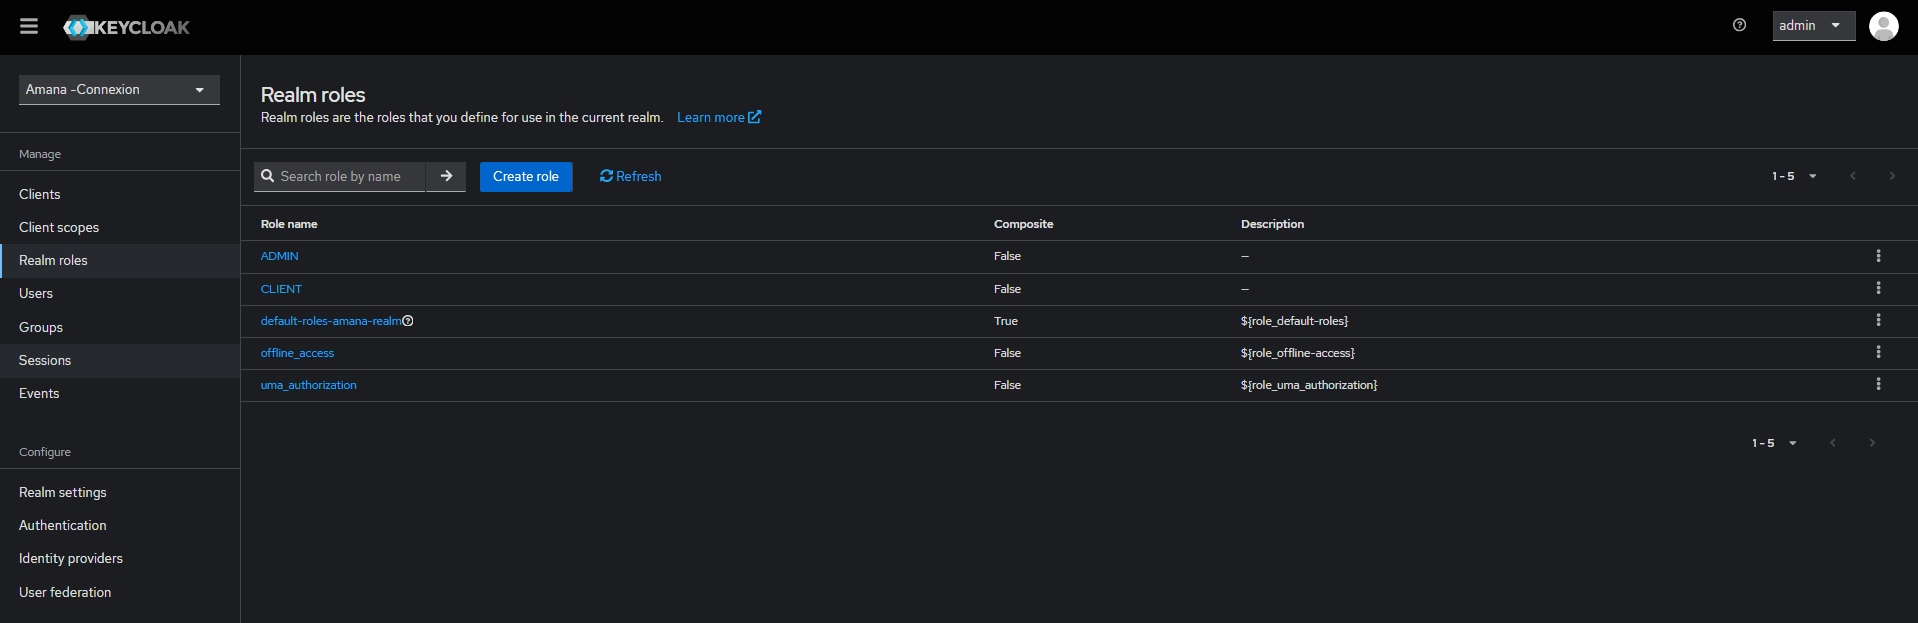
\includegraphics[width=0.8\textwidth]{images/keycloak_roles.png}
\caption{Gestion des rôles utilisateur dans Keycloak}
\label{fig:keycloak_roles}
\end{figure}

La Figure \ref{fig:keycloak_roles} détaille la gestion des rôles dans Keycloak. Les rôles CLIENT et ADMIN déterminent les autorisations d'accès aux données et fonctionnalités. Cette gestion fine des permissions garantit l'isolation des données clients et la sécurité globale du système.

\subsubsection{Protection des endpoints}

La protection des endpoints utilise Spring Security avec validation automatique des tokens JWT. Chaque requête est interceptée pour vérifier l'authenticité du token, extraire les informations utilisateur, et valider les autorisations d'accès aux ressources demandées.

\section{Intégration MongoDB}

\subsection{Configuration MongoDB}

\begin{figure}[H]
\centering
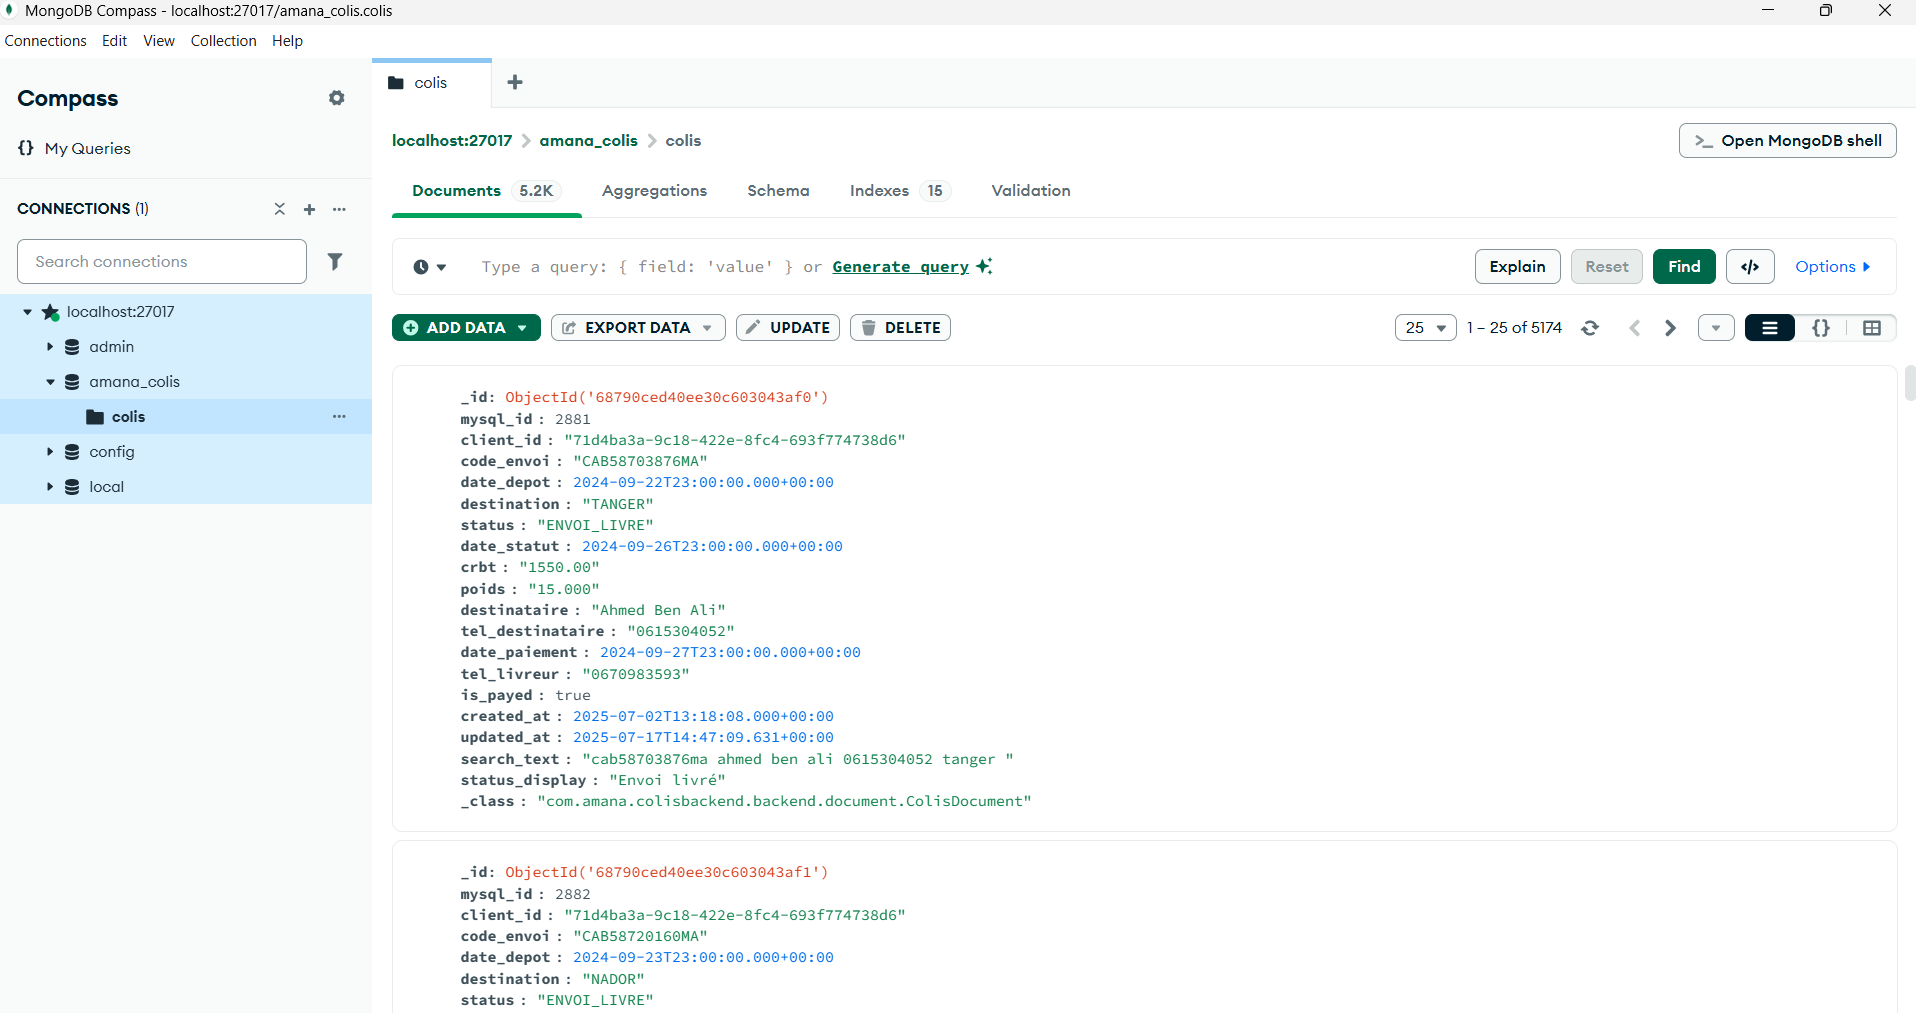
\includegraphics[width=1.0\textwidth]{images/mongodb_compass.png}
\caption{Interface MongoDB Compass - Gestion des collections}
\label{fig:mongodb_compass}
\end{figure}

La Figure \ref{fig:mongodb_compass} montre l'interface MongoDB Compass [20] utilisée pour la gestion et le monitoring de la base de données documentaire. L'outil permet de visualiser la structure des documents, gérer les index, et surveiller les performances des requêtes en temps réel.

\subsection{Modèles de documents}

La structure des documents MongoDB a été optimisée pour les performances de lecture avec des champs calculés et une dénormalisation appropriée. Les documents incluent les données métier essentielles ainsi que des champs optimisés pour la recherche et la visualisation.

\subsection{Repositories MongoDB}

\begin{figure}[H]
\centering
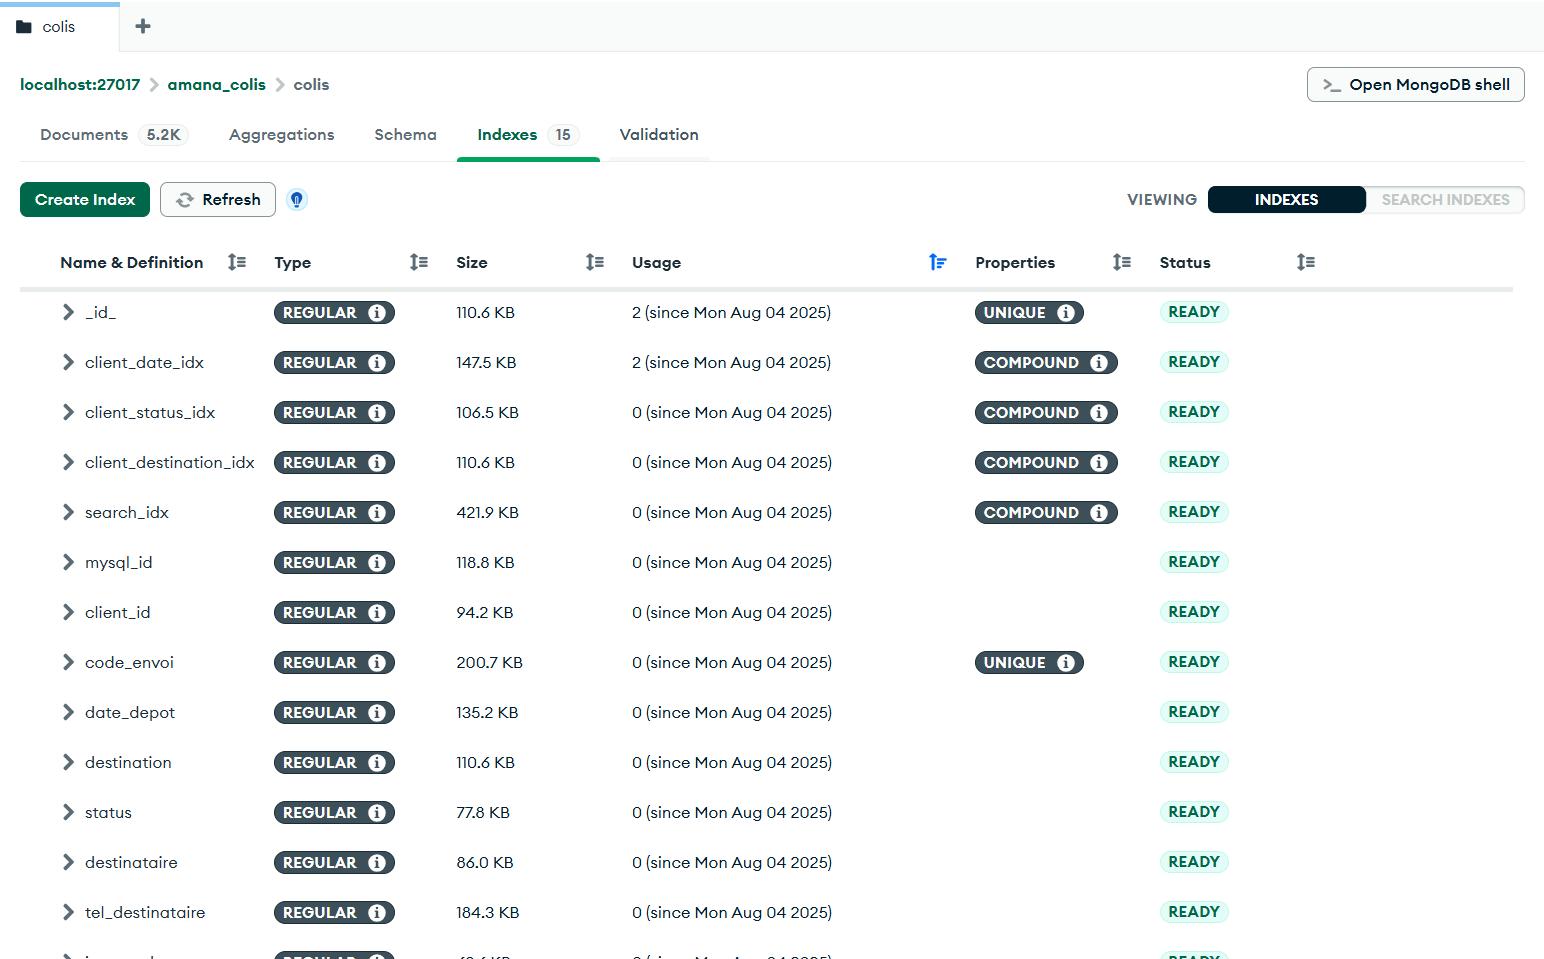
\includegraphics[width=1.0\textwidth]{images/mongodb_indexes.png}
\caption{Index MongoDB pour optimisation des performances}
\label{fig:mongodb_indexes}
\end{figure}

La Figure \ref{fig:mongodb_indexes} détaille la stratégie d'indexation MongoDB avec les index composés, textuels, et géospatiaux. Cette indexation spécialisée optimise les performances selon les patterns d'usage identifiés : consultation par client, recherche full-text, et requêtes géographiques.
\section{Développement Frontend}

\subsection{Interface utilisateur React}

\begin{figure}[H]
\centering
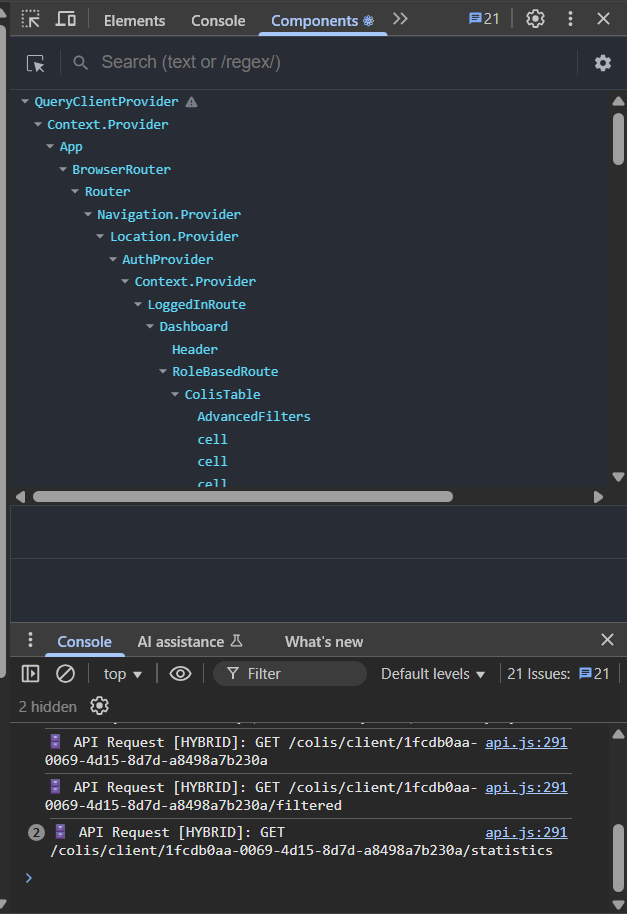
\includegraphics[width=0.7\textwidth]{images/react_dev_tools.png}
\caption{Développement React avec DevTools}
\label{fig:react_dev_tools}
\end{figure}

La Figure \ref{fig:react_dev_tools} montre l'environnement de développement React avec les DevTools permettant l'inspection des composants, la gestion des états, et le debugging des performances. Cette tooling avancée facilite le développement et l'optimisation de l'interface utilisateur.

\subsection{Intégration Keycloak Frontend}

\begin{figure}[H]
\centering
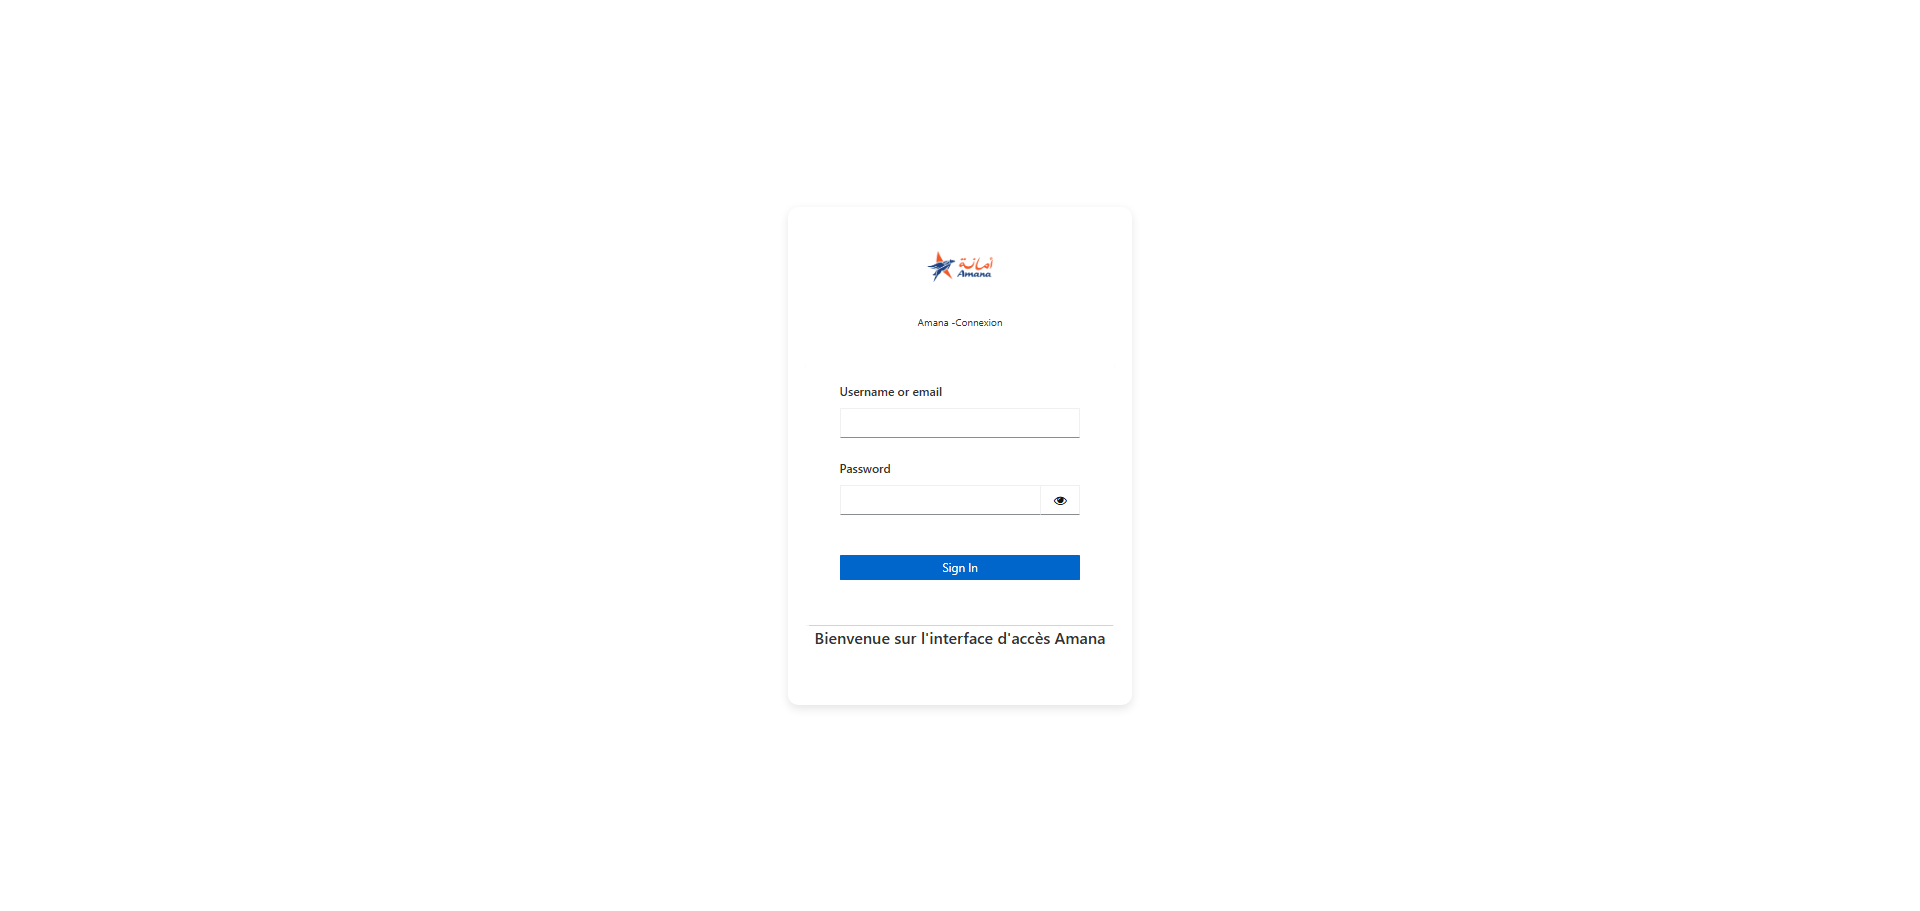
\includegraphics[width=0.7\textwidth]{images/keycloak_login.png}
\caption{Interface de connexion Keycloak}
\label{fig:keycloak_login}
\end{figure}

La Figure \ref{fig:keycloak_login} présente l'interface de connexion Keycloak intégrée dans l'application. Cette interface sécurisée gère l'authentification utilisateur avec support des standards OAuth 2.0 et OpenID Connect, offrant une expérience utilisateur fluide et sécurisée.

\subsection{Composants de visualisation}

L'architecture des composants React suit une approche modulaire avec séparation claire entre composants de présentation et composants containers. Cette organisation facilite la réutilisabilité, les tests, et la maintenance du code frontend.

\subsection{Intégration cartographique}

\begin{figure}[H]
\centering
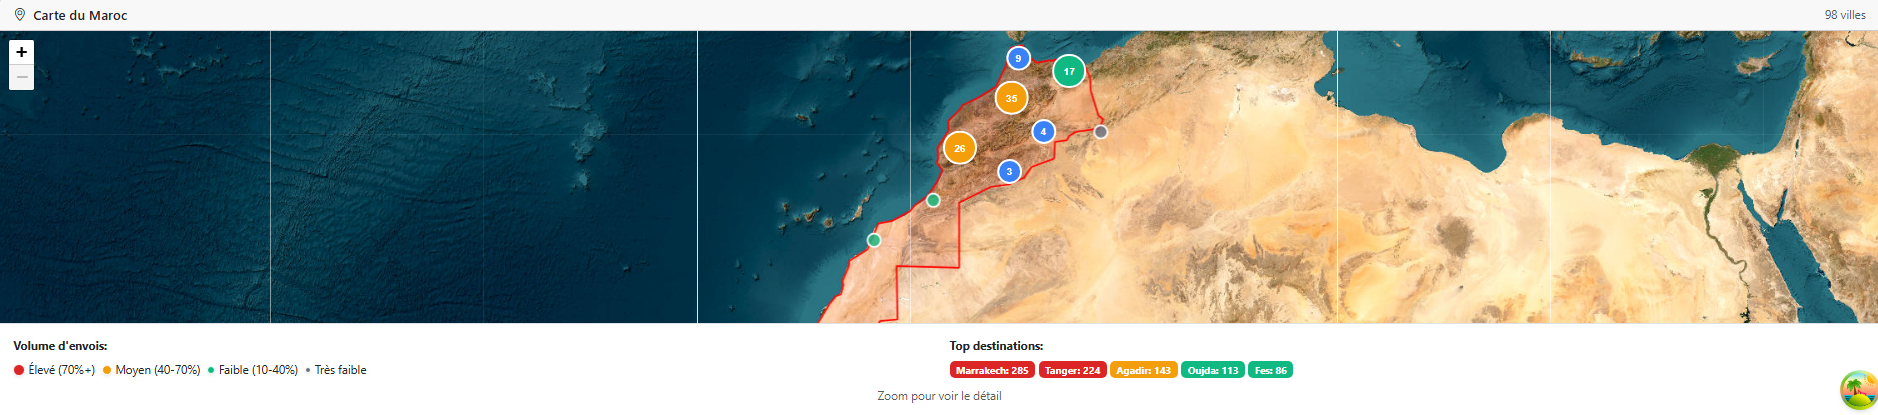
\includegraphics[width=1.0\textwidth]{images/leaflet_integration.png}
\caption{Intégration cartographique avec Leaflet}
\label{fig:leaflet_integration}
\end{figure}

La Figure \ref{fig:leaflet_integration} présente l'intégration cartographique utilisant Leaflet avec tiles haute résolution et clustering intelligent. Cette implémentation remplace l'affichage GeoJSON basique par une solution performante capable de gérer des milliers de points simultanément avec des performances optimales.

\subsection{Gestion des états}

La gestion des états utilise React Context pour les données globales (authentification, configuration) et useState/useEffect pour les états locaux des composants. Cette approche équilibrée évite la complexité excessive tout en maintenant la performance et la maintenabilité.

\section{Fonctionnalités Implémentées}

\subsection{Gestion des colis}

\begin{figure}[H]
\centering
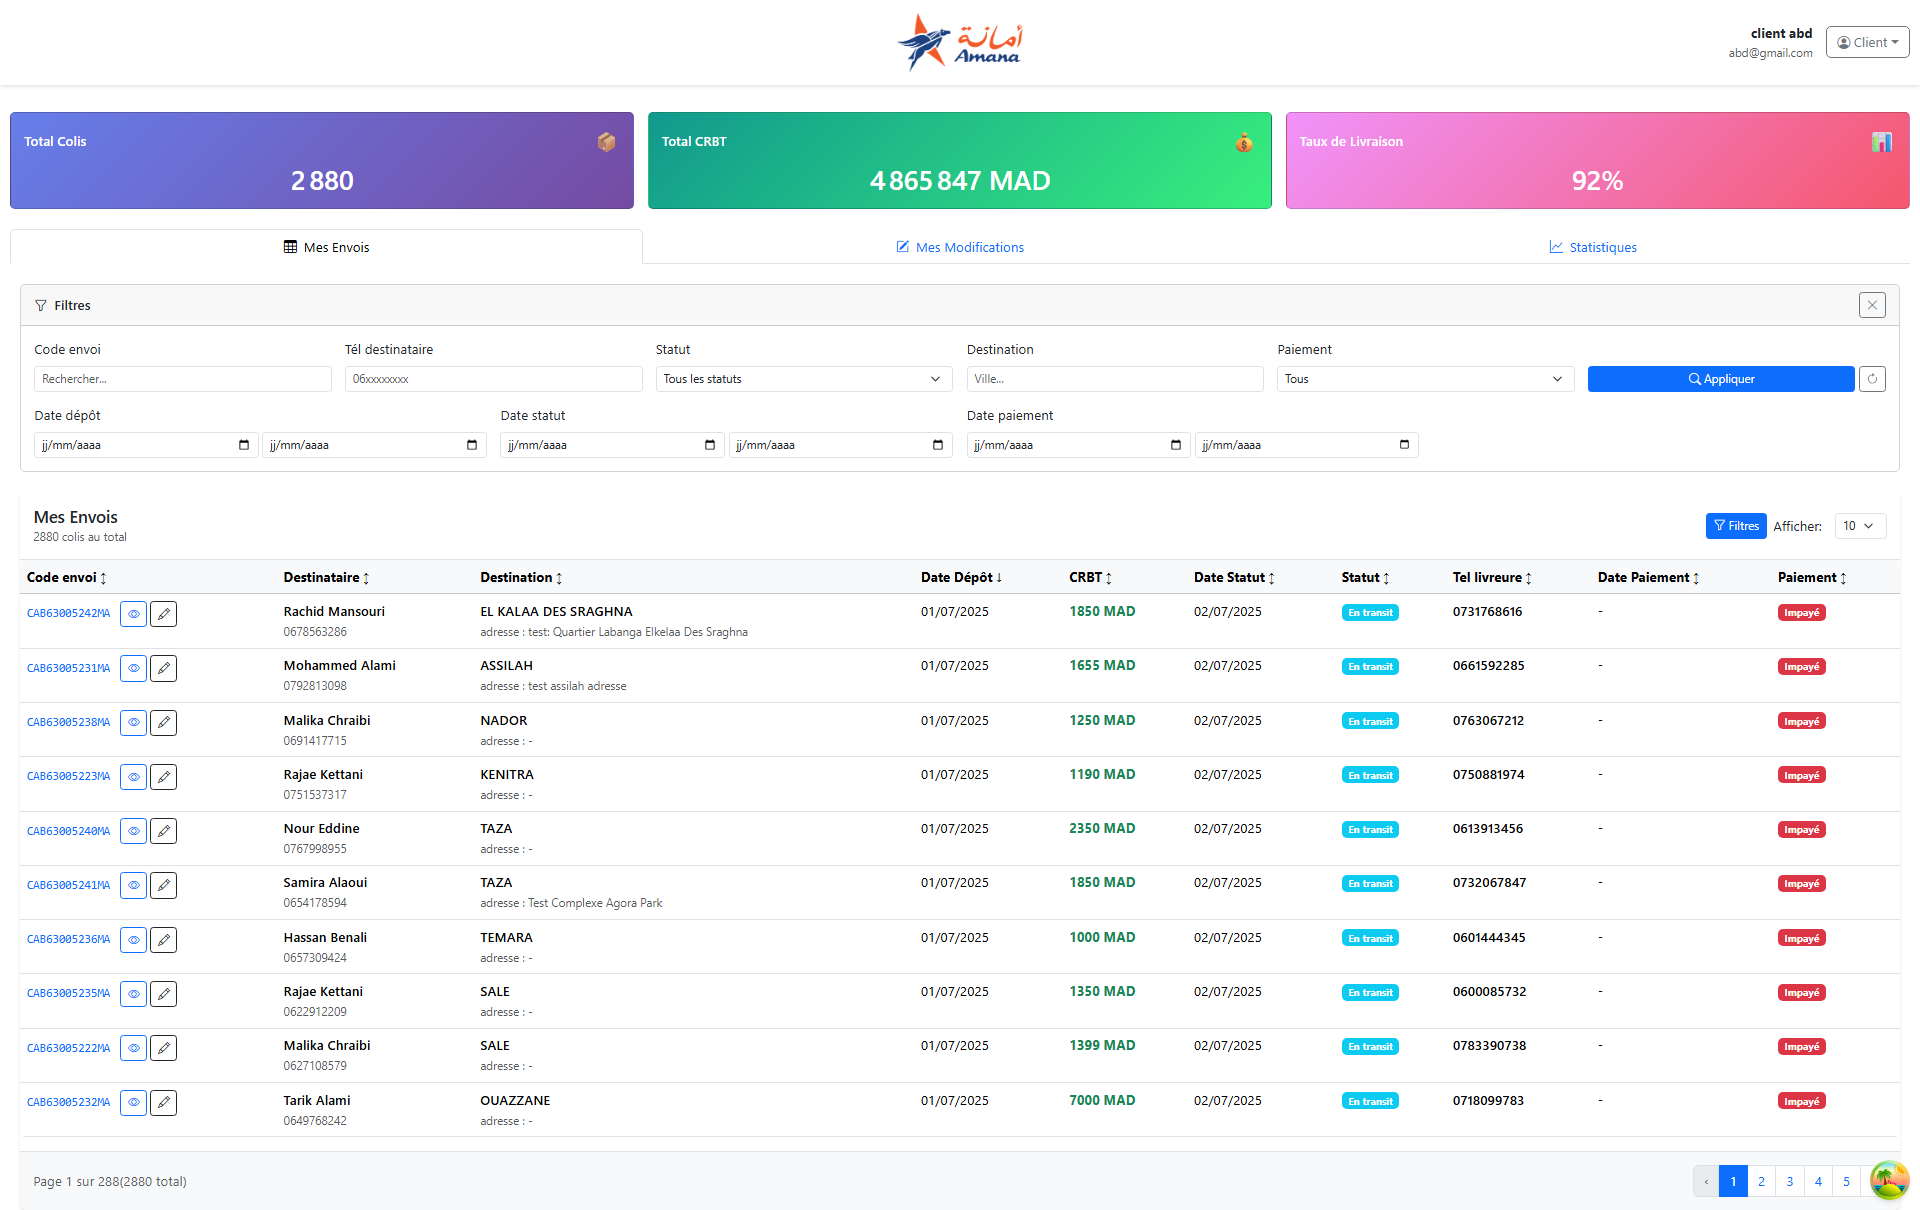
\includegraphics[width=1.0\textwidth]{images/colis_list_interface.png}
\caption{Interface de gestion des colis}
\label{fig:colis_list_interface}
\end{figure}

La Figure \ref{fig:colis_list_interface} montre l'interface principale de gestion des colis avec pagination optimisée, filtres avancés, et recherche intelligente. Cette interface exploite les performances MongoDB pour offrir une expérience utilisateur fluide même avec de gros volumes de données.

\subsection{Tableaux de bord}

\begin{figure}[H]
\centering
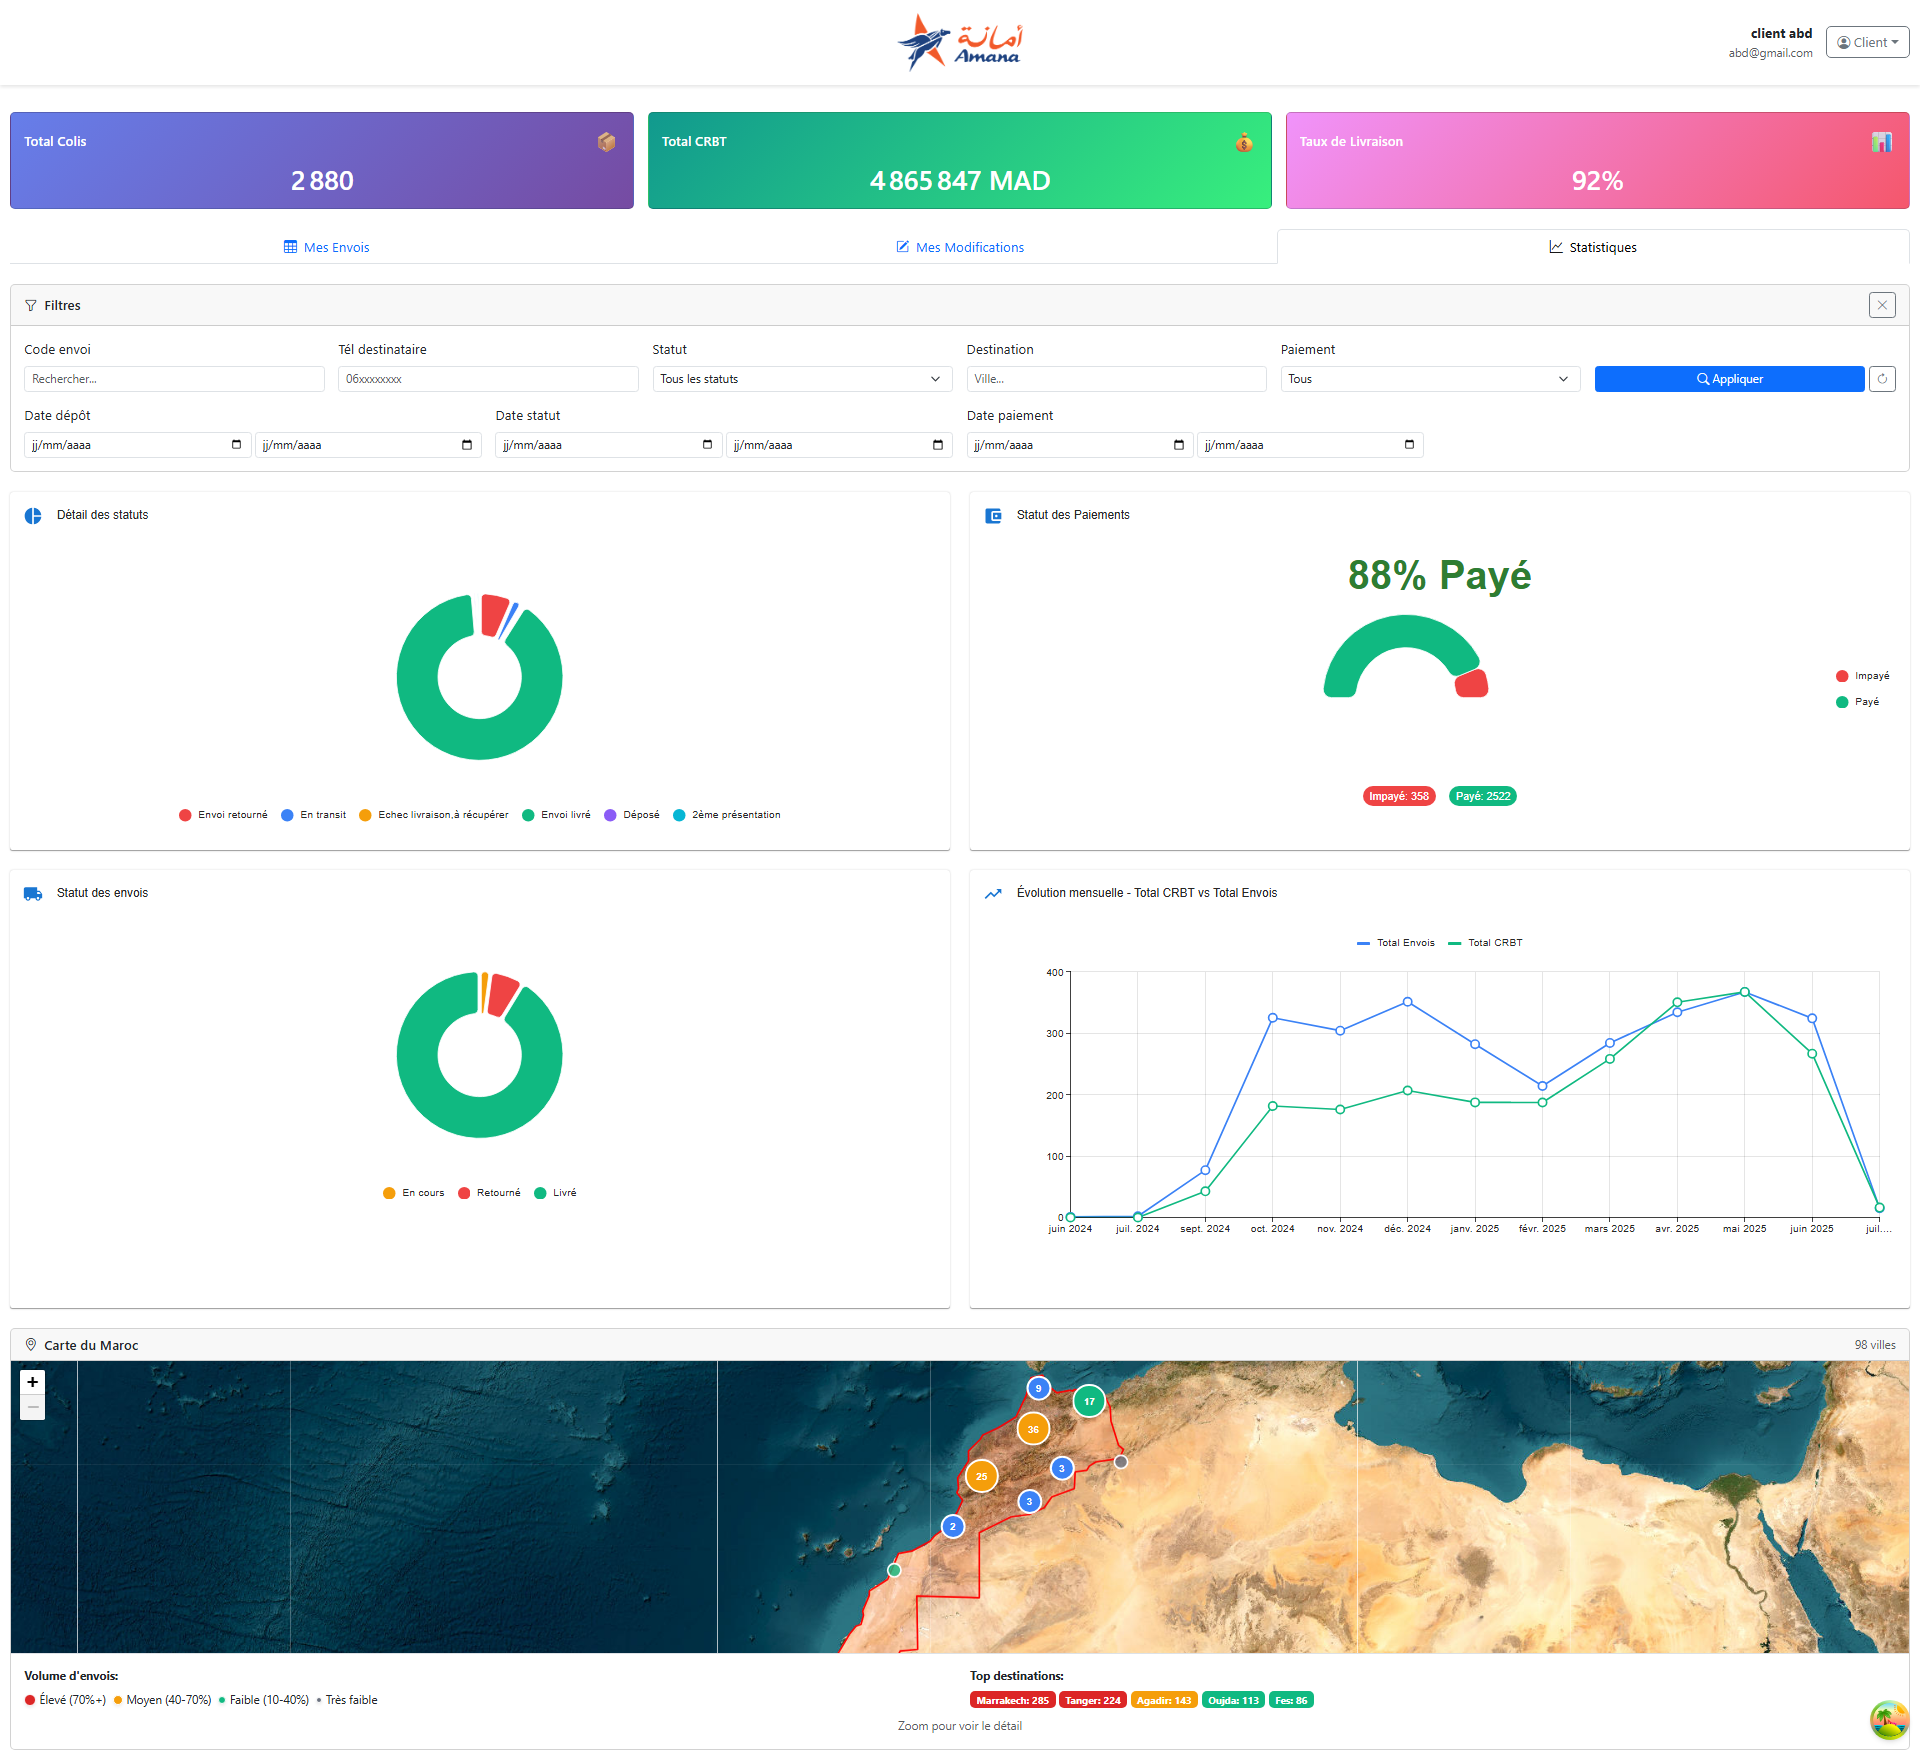
\includegraphics[width=1.0\textwidth]{images/dashboard_interface.png}
\caption{Tableaux de bord avec statistiques temps réel}
\label{fig:dashboard_interface}
\end{figure}

La Figure \ref{fig:dashboard_interface} illustre les tableaux de bord offrant une vue synthétique de l'activité avec graphiques interactifs et métriques en temps réel. Ces dashboards s'adaptent selon le profil utilisateur (client ou administrateur) pour présenter les informations pertinentes.

\subsection{Gestion des modifications}

\begin{figure}[H]
\centering
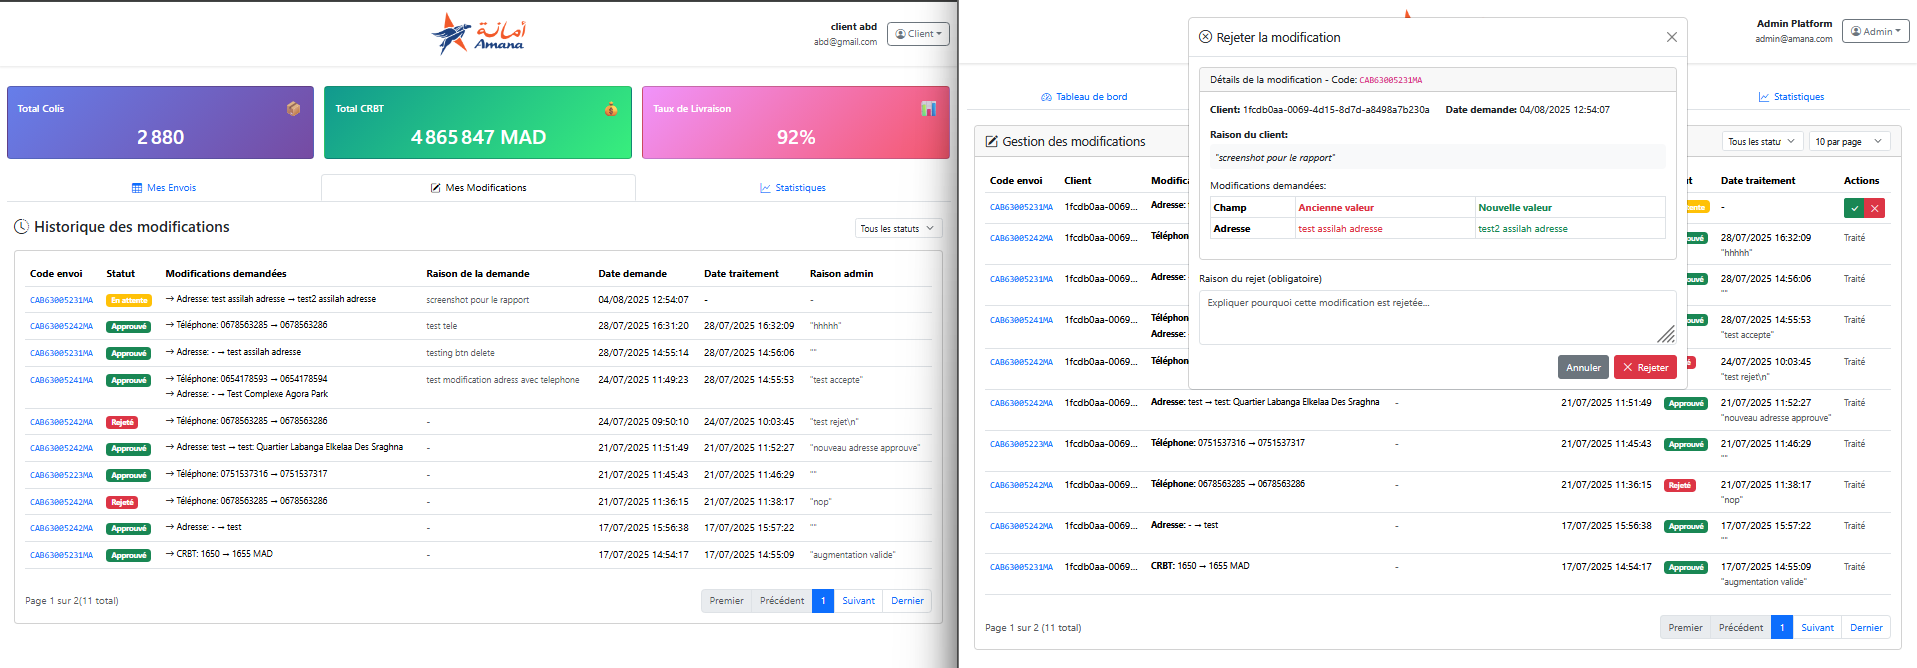
\includegraphics[width=1.0\textwidth]{images/modifications_workflow.png}
\caption{Interface de gestion des modifications - Workflow d'approbation}
\label{fig:modifications_workflow}
\end{figure}
La Figure \ref{fig:modifications_workflow} présente le système de gestion des demandes de modification avec workflow d'approbation. Cette interface permet aux clients de soumettre des demandes de changement et aux administrateurs de les valider ou rejeter avec traçabilité complète des actions effectuées.

\subsection{Interface administrateur}

\begin{figure}[H]
\centering
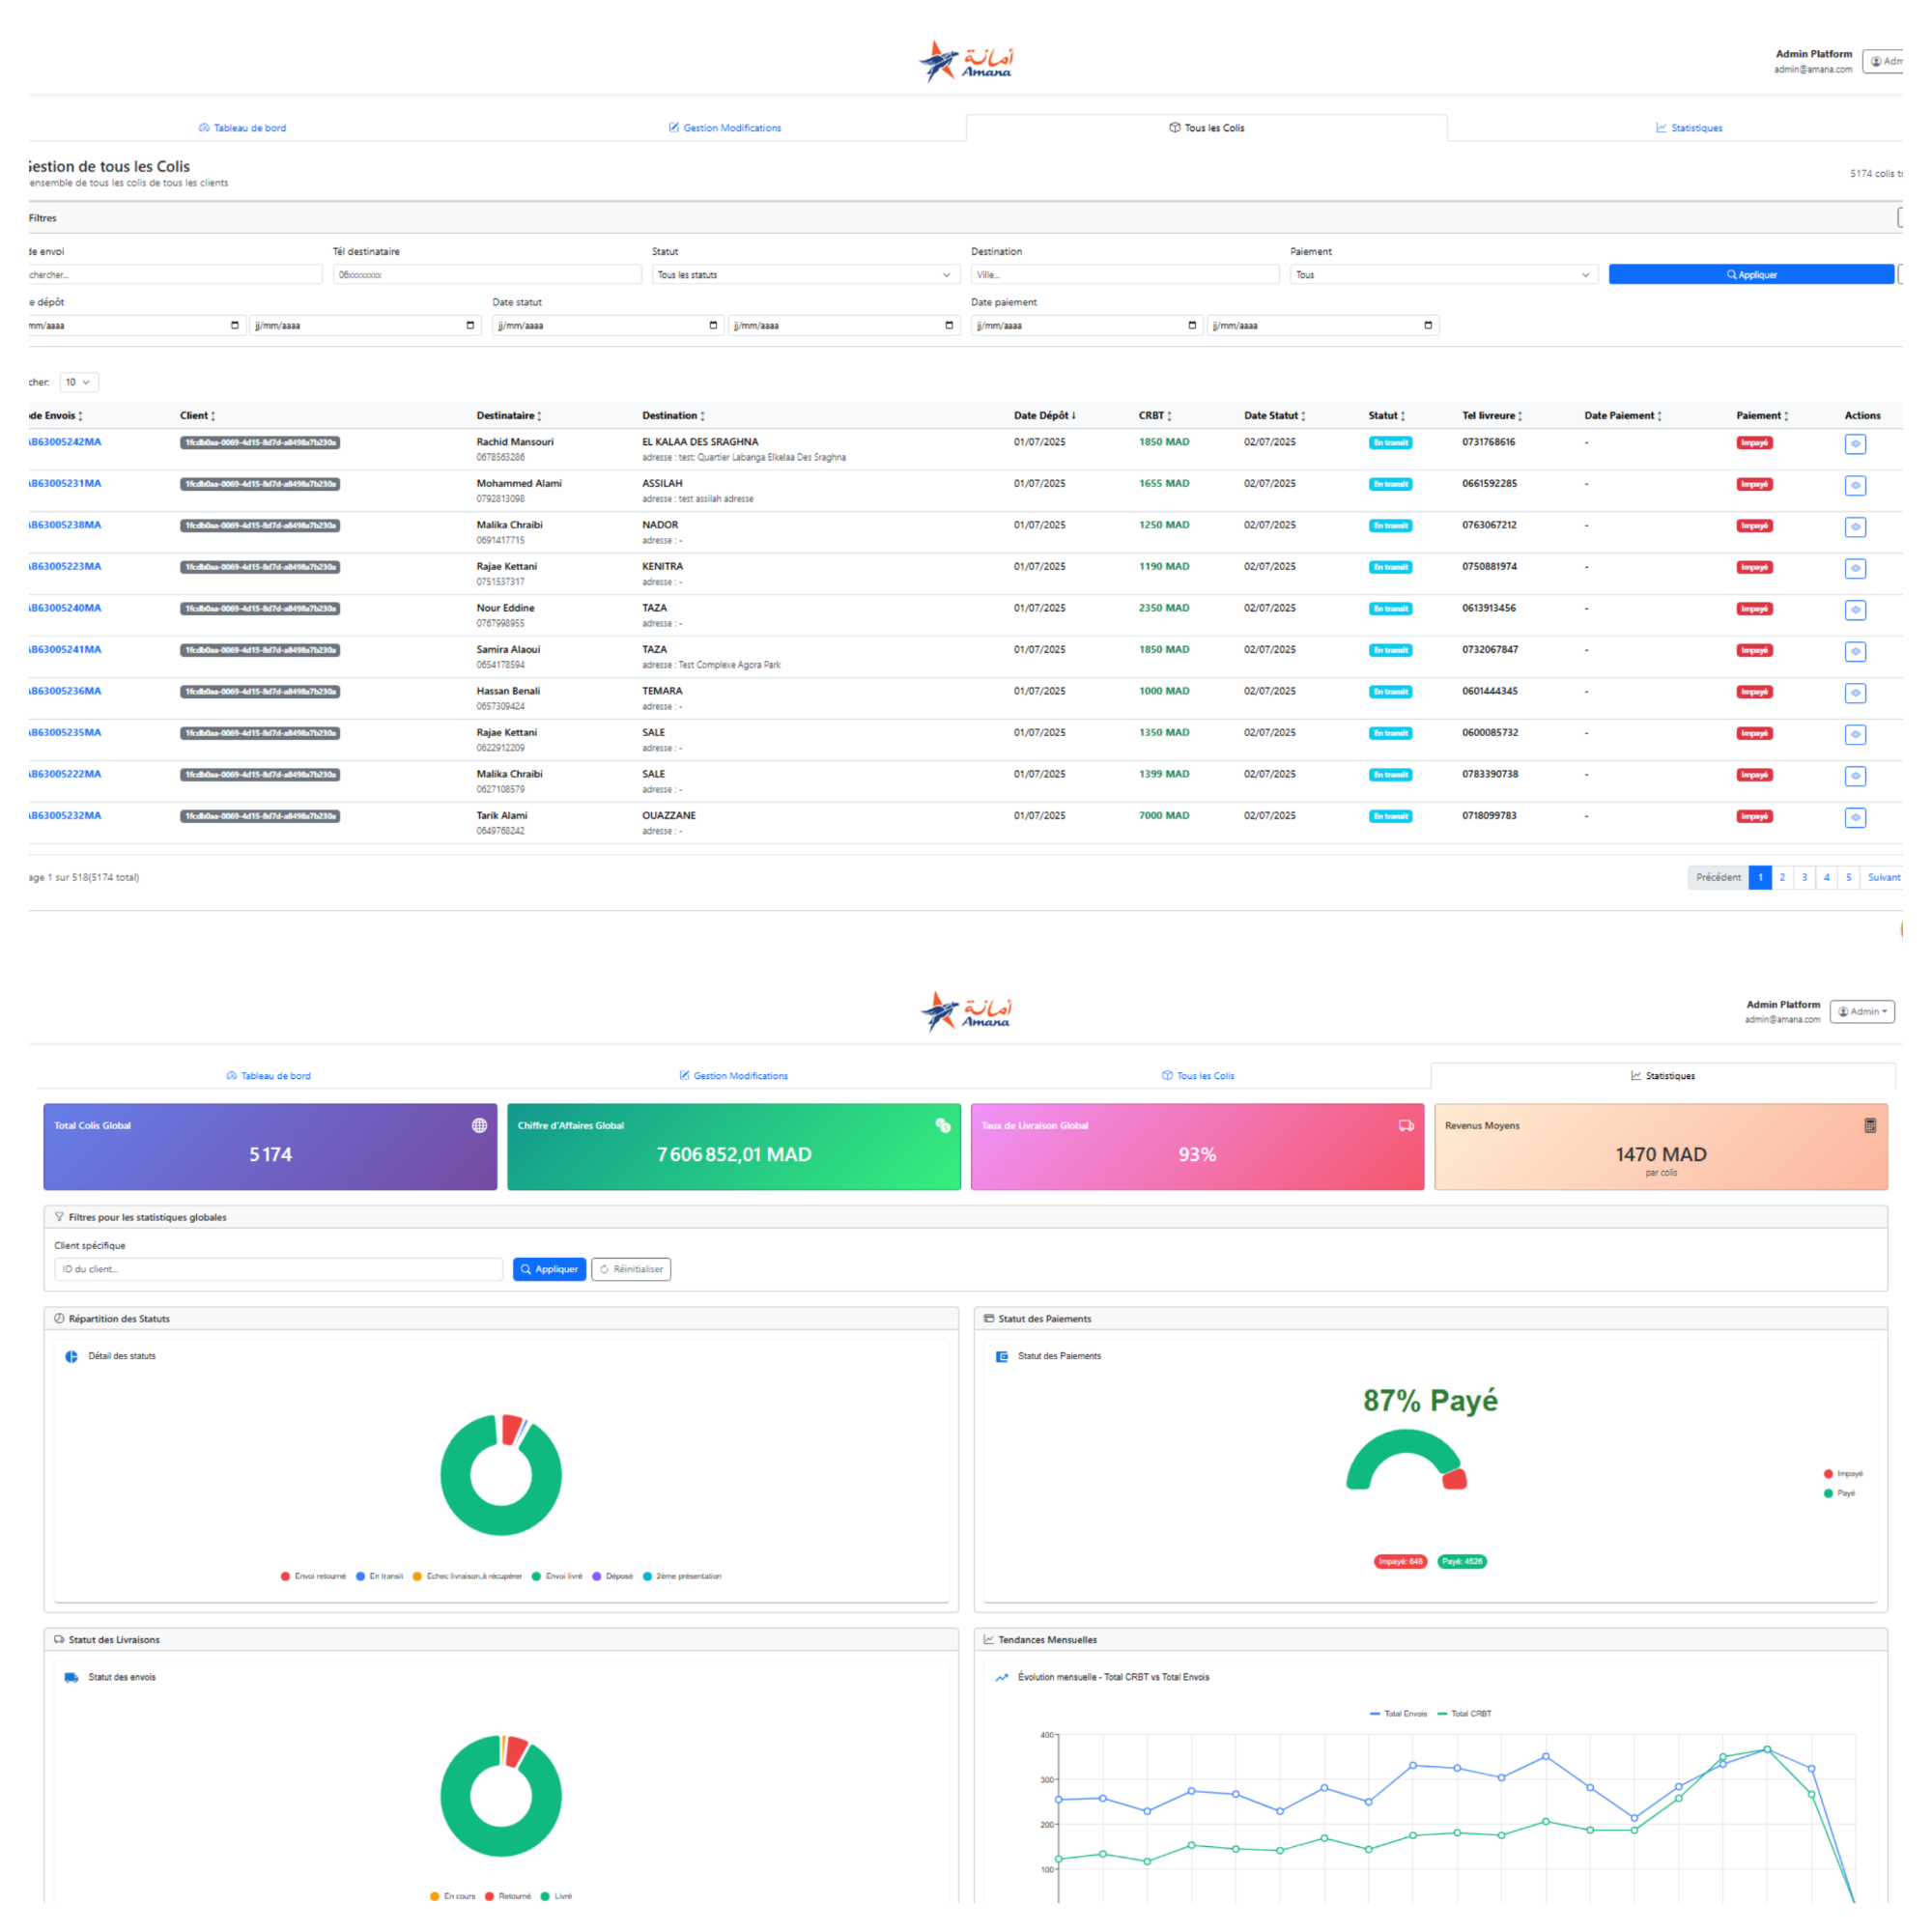
\includegraphics[width=0.6\textwidth]{images/admin_interface.png}
\caption{Interface administrateur - Vue globale du système}
\label{fig:admin_interface}
\end{figure}

La Figure \ref{fig:admin_interface} montre l'interface administrateur offrant une vue globale sur l'ensemble des données du système. Cette interface permet la supervision de tous les clients, la gestion des demandes de modification, et l'accès aux statistiques globales de performance.

% Partie 8 : Réflexion et Perspectives
\chapter{Réflexion et Perspectives}

\section{Bilan du Stage}

\subsection{Objectifs atteints}

Cette mission de six semaines au sein de Barid Al Maghrib a permis d'atteindre l'ensemble des objectifs fixés lors de sa définition initiale. Le système de gestion des colis postaux a été entièrement modernisé selon une approche d'ingénieur méthodique, alliant analyse rigoureuse des besoins, conception d'architectures innovantes, et implémentation technique maîtrisée.

L'objectif principal de développement d'une architecture hybride MySQL/MongoDB a été atteint avec succès. Cette innovation technique a permis d'exploiter les avantages de chaque technologie : MySQL pour la gestion transactionnelle critique et MongoDB pour l'optimisation des requêtes de consultation et de recherche. Cette dualité architecturale constitue une réponse adaptée aux contraintes de performance identifiées dans le système existant.

Le renouvellement complet du système de visualisation cartographique représente une réussite technique majeure. Le passage d'un affichage basique de frontières GeoJSON vers une solution avancée intégrant des tiles haute résolution et un clustering intelligent a transformé radicalement l'expérience utilisateur. Cette modernisation apporte désormais une dimension véritablement professionnelle au suivi géographique des colis.

L'intégration de Keycloak comme solution d'authentification enterprise constitue également un succès notable. La mise en œuvre d'une gestion des rôles (ADMIN, CLIENT), de la protection JWT des API, et de l'intégration transparente côté frontend React garantit désormais un niveau de sécurité conforme aux standards industriels.
\subsection{Résultats quantifiables}

Les améliorations apportées au système se traduisent par des gains mesurables et une validation concrète de l'efficacité des solutions implémentées.

\begin{table}[H]
\centering
\caption{Résultats quantifiés du projet d'optimisation}
\label{tab:resultats_quantifies}
\resizebox{\textwidth}{!}{
\begin{tabular}{|l|l|l|l|l|}
\hline
\textbf{Métrique} & \textbf{Avant} & \textbf{Après} & \textbf{Amélioration} & \textbf{Validation} \\
\hline
Temps de réponse listings & 3-5 secondes & < 1 seconde & -75\% & Tests de charge \\
\hline
Affichage cartographique & Statique & Interactif HR & Transformation & Tests utilisateur \\
\hline
Authentification & Spring Security basique & Keycloak OAuth2 + JWT & Sécurité renforcée & Tests Postman \\
\hline
Gestion des rôles & Limitée & ADMIN/CLIENT & Contrôle d'accès fin & Tests autorisations \\
\hline
Planning & 6 semaines & 6 semaines & 100\% respecté & Livraison complète \\
\hline
Fonctionnalités & 100\% prévues & 100\% livrées & Objectifs atteints & Tests validation \\
\hline
\end{tabular}
}
\end{table}


L'ensemble des fonctionnalités principales ont été développées, testées et validées dans les délais impartis, témoignant de l'efficacité de la méthodologie adoptée.

\subsection{Impact sur l'organisation}

Bien que le projet s'inscrive dans une logique essentiellement pédagogique, les solutions développées apportent une contribution concrète à Barid Al Maghrib en démontrant la faisabilité technique d'approches architecturales innovantes pour l'optimisation des systèmes d'information.

L'architecture hybride MySQL/MongoDB constitue un proof-of-concept précieux pour l'organisation, illustrant comment exploiter les technologies NoSQL pour améliorer les performances sans compromettre la robustesse transactionnelle. Cette approche peut inspirer d'autres projets d'optimisation au sein de l'entreprise.

La modernisation de la visualisation cartographique démontre l'importance de l'expérience utilisateur dans l'efficacité opérationnelle. Cette réalisation peut servir de référence pour l'amélioration d'autres interfaces utilisateur au sein de l'organisation.

L'intégration de Keycloak illustre concrètement les bénéfices d'une approche centralisée de la gestion des identités et des accès. Cette expérience peut éclairer les décisions d'architecture pour les futurs projets enterprise de Barid Al Maghrib.

\section{Apport Personnel}

\subsection{Développement professionnel}

Cette expérience a considérablement enrichi mon profil professionnel en me confrontant aux réalités techniques et organisationnelles du développement de systèmes d'information enterprise. La gestion d'un projet complet a renforcé ma capacité d'autonomie et ma méthodologie de travail.

\begin{table}[H]
\centering
\caption{Synthèse des compétences techniques développées}
\label{tab:competences_developpees}
\begin{tabular}{|l|p{4cm}|p{3cm}|p{4cm}|}
\hline
\textbf{Domaine} & \textbf{Technologies maîtrisées} & \textbf{Niveau acquis} & \textbf{Apport professionnel} \\
\hline
\multirow{3}{*}{\textbf{Backend}} & Spring Boot 3.1 & Intermédiaire+ & Frameworks enterprise Java \\
\cline{2-4}
& Spring Security 6.1 & Intermédiaire & Sécurité OAuth2/JWT \\
\cline{2-4}
& Spring Data (JPA/MongoDB) & Intermédiaire & Architectures de données hybrides \\
\hline
\multirow{2}{*}{\textbf{Frontend}} & React 18.2 & Intermédiaire+ & Interfaces modernes et interactives \\
\cline{2-4}
& Leaflet + React-Leaflet & Débutant+ & Géoinformation et visualisation spatiale \\
\hline
\multirow{2}{*}{\textbf{Bases de données}} & MySQL 8.0 & Intermédiaire & Persistance relationnelle \\
\cline{2-4}
& MongoDB 6.0 & Débutant+ & NoSQL et optimisation performances \\
\hline
\textbf{Sécurité} & Keycloak 23.0 & Débutant+ & IAM enterprise et standards OAuth \\
\hline
\multirow{2}{*}{\textbf{DevOps}} & Docker & Intermédiaire+ & Conteneurisation des services \\
\cline{2-4}
& Git/GitHub Projects & Intermédiaire+ & Gestion de projet Agile \\
\hline
\end{tabular}
\end{table}

Cette polyvalence technique constitue un atout précieux dans un environnement professionnel où la maîtrise de stacks technologiques diversifiées devient indispensable.
\subsection{Vision ingénieur}

Ce stage a profondément influencé ma vision du métier d'ingénieur informatique en me confrontant aux défis réels de l'optimisation de systèmes en production. La nécessité de concilier performance, sécurité, maintenabilité et expérience utilisateur a développé ma capacité d'analyse systémique et ma compréhension des compromis techniques.

L'expérience de conception d'une architecture hybride m'a sensibilisé à l'importance de l'adaptabilité technologique. La capacité à évaluer et intégrer différentes technologies selon leurs forces respectives constitue une compétence essentielle de l'ingénieur moderne face à l'évolution rapide des écosystèmes technologiques.

La prise en compte des contraintes opérationnelles de Barid Al Maghrib a renforcé ma compréhension de l'importance du contexte métier dans les choix techniques. Cette approche pragmatique, privilégiant l'efficacité opérationnelle aux considérations purement techniques, caractérise la démarche d'ingénieur responsable.

La gestion de la complexité technique tout en préservant la simplicité d'usage pour les utilisateurs finaux a développé ma sensibilité aux enjeux d'ergonomie et d'expérience utilisateur. Cette préoccupation de l'usage constitue un élément différenciant crucial pour l'ingénieur dans la conception de solutions technologiques.

\subsection{Compétences transversales}

Au-delà des compétences techniques spécialisées, cette expérience a développé mes capacités transversales indispensables à l'exercice du métier d'ingénieur. La gestion de projet en autonomie complète, de la planification initiale à la livraison finale, a renforcé mes compétences organisationnelles et ma capacité de priorisation.

L'adaptation à l'environnement professionnel de Barid Al Maghrib a développé mes compétences relationnelles et ma capacité d'intégration dans une équipe technique. Les échanges réguliers avec mon encadrant technique ont enrichi ma compréhension des dynamiques de collaboration dans les projets informatiques.

La documentation technique produite tout au long du projet a consolidé mes compétences de communication écrite, particulièrement importantes pour la transmission des connaissances et la pérennité des solutions développées. Cette capacité de formalisation constitue un élément essentiel de la démarche d'ingénieur.

La résolution de problèmes complexes, notamment lors de l'intégration de technologies hétérogènes, a développé ma capacité d'analyse et ma créativité technique. Cette agilité intellectuelle représente un atout précieux face aux défis techniques variés que rencontre l'ingénieur informatique.

\section{Perspectives d'Évolution}

\subsection{Améliorations possibles}

Plusieurs axes d'amélioration peuvent être identifiés pour enrichir les fonctionnalités du système et optimiser davantage ses performances. L'implémentation d'un système de cache distribué avec Redis pourrait améliorer significativement les temps de réponse des requêtes fréquentes, particulièrement bénéfique lors des pics d'activité de consultation.

L'enrichissement des fonctionnalités de recherche par l'intégration d'Elasticsearch constituerait une évolution majeure. Cette technologie apporterait des capacités de recherche full-text avancées, des suggestions automatiques, et des fonctionnalités d'analyse textuelle sophistiquées particulièrement adaptées au traitement des adresses postales.

L'optimisation de l'interface utilisateur par l'implémentation de fonctionnalités avancées comme la virtualisation des listes longues, le lazy loading des données cartographiques, et l'amélioration de la responsivité mobile représentent des pistes d'amélioration prioritaires pour l'expérience utilisateur.

L'ajout de fonctionnalités de monitoring et d'observabilité avec des solutions comme Prometheus et Grafana permettrait un suivi opérationnel professionnel du système, facilitant l'identification proactive des problèmes de performance et la maintenance préventive.

\subsection{Évolutions technologiques}

L'écosystème technologique évolue rapidement et plusieurs tendances peuvent influencer les futures évolutions du système. L'adoption de l'architecture microservices avec Spring Cloud pourrait améliorer la scalabilité et la résilience du système, permettant un déploiement et une montée en charge plus flexibles.

L'intégration de technologies d'intelligence artificielle pour l'amélioration automatique de la qualité des données d'adresses représente une perspective d'évolution prometteuse. Les algorithmes de machine learning pourraient détecter et corriger automatiquement les erreurs d'adresses, améliorant la qualité globale du système.

L'adoption de technologies de containerisation avec Kubernetes permettrait une gestion plus sophistiquée du déploiement et de l'orchestration des services, particulièrement adaptée aux besoins de scalabilité de Barid Al Maghrib.

L'évolution vers des architectures serverless pour certaines fonctionnalités, notamment le traitement des données géographiques et la génération de rapports, pourrait optimiser les coûts d'infrastructure et améliorer l'élasticité du système.


% Conclusion Générale
\chapter*{Conclusion Générale}
\addcontentsline{toc}{chapter}{Conclusion Générale}

Ce stage de six semaines au sein de Barid Al Maghrib a constitué une expérience formatrice exceptionnelle, me permettant de mettre en œuvre concrètement les compétences d'ingénieur informatique acquises durant ma formation à l'EMSI. Cette mission s'est révélée être bien plus qu'un simple exercice académique, en me confrontant aux défis réels de l'optimisation de systèmes d'information dans le contexte exigeant du secteur logistique et postal.

Le projet de développement et d'optimisation du système de gestion des colis postaux a permis de démontrer l'efficacité d'une approche d'ingénieur méthodique face à des problématiques techniques complexes. Les limitations initiales du système existant - performances dégradées, visualisation cartographique basique, et sécurisation insuffisante - ont été transformées en opportunités d'innovation technique et d'amélioration significative de l'expérience utilisateur.

Les trois axes principaux d'innovation développés illustrent la richesse des solutions techniques modernes applicables aux enjeux du secteur postal. L'architecture hybride MySQL/MongoDB a démontré qu'il est possible d'optimiser drastiquement les performances tout en préservant la robustesse transactionnelle critique. Cette approche pragmatique constitue un modèle applicable à d'autres contextes où la conciliation entre performance et fiabilité représente un enjeu majeur.

La modernisation complète du système de visualisation cartographique, avec l'intégration de tiles haute résolution et de clustering intelligent, a transformé radicalement l'expérience utilisateur. Cette évolution démontre l'impact considérable que peuvent avoir les innovations d'interface sur l'efficacité opérationnelle des utilisateurs finaux. Le passage d'un affichage statique vers une solution interactive professionnelle illustre l'importance de l'ergonomie dans la conception de systèmes d'information contemporains.

L'implémentation de Keycloak comme solution d'authentification enterprise a établi un niveau de sécurité conforme aux standards industriels, avec une gestion fine des rôles et une protection JWT robuste des API. Cette réalisation souligne l'importance cruciale de la sécurisation dans les systèmes traitant des données sensibles et démontre la faisabilité d'intégration de solutions enterprise dans des contextes opérationnels complexes.

Au-delà des contributions techniques spécifiques, cette expérience a profondément enrichi ma vision du métier d'ingénieur informatique. La nécessité de concilier exigences techniques, contraintes opérationnelles, et besoins utilisateur a développé ma compréhension des compromis inhérents à la conception de systèmes d'information. Cette approche systémique, privilégiant l'efficacité globale aux optimisations locales, constitue un acquis fondamental pour ma future pratique professionnelle.

La gestion complète du cycle de développement, de l'analyse des besoins à la livraison d'un système fonctionnel, a consolidé mes compétences organisationnelles et ma capacité d'autonomie. Cette expérience de responsabilité technique individuelle représente un facteur déterminant dans ma maturation professionnelle et ma confiance dans la gestion de projets complexes.

L'approfondissement technique réalisé dans des domaines variés - développement backend Spring Boot, développement frontend React, gestion de bases de données hybrides, sécurisation enterprise avec Keycloak - a considérablement élargi mon spectre de compétences. Cette polyvalence technique constitue un atout précieux dans un environnement professionnel où la maîtrise de stacks technologiques diversifiées devient indispensable.

La collaboration avec les équipes techniques de Barid Al Maghrib a également enrichi ma compréhension des dynamiques de travail en environnement enterprise. L'adaptation aux processus organisationnels, aux contraintes de sécurité, et aux exigences de qualité propres au secteur postal a développé ma capacité d'intégration professionnelle.

Cette expérience confirme l'importance de l'approche pratique dans la formation d'ingénieur, complétant efficacement les acquisitions théoriques par une confrontation aux réalités techniques et organisationnelles. La transition entre formation académique et exercice professionnel s'effectue naturellement lorsque les projets proposés offrent une complexité technique suffisante et une autonomie de réalisation appropriée.

Les perspectives d'évolution identifiées dans ce rapport témoignent de la richesse des possibilités d'amélioration et d'innovation dans le domaine des systèmes d'information postaux. L'adoption de technologies émergentes comme l'intelligence artificielle pour l'amélioration automatique de la qualité des données, ou l'évolution vers des architectures microservices pour une meilleure scalabilité, ouvre des horizons prometteurs pour l'optimisation continue des systèmes.

Cette mission au sein de Barid Al Maghrib s'inscrit parfaitement dans la continuité de ma formation et constitue une transition réussie vers l'exercice professionnel du métier d'ingénieur informatique. Les compétences développées, la confiance acquise, et la vision enrichie du métier constituent un socle solide pour aborder les défis techniques qui caractériseront ma future carrière professionnelle.

Enfin, cette expérience illustre la pertinence des partenariats entre institutions de formation et entreprises pour offrir aux étudiants ingénieurs des opportunités d'application concrète de leurs compétences. La qualité de l'encadrement technique et la richesse des projets proposés par Barid Al Maghrib démontrent l'engagement de l'organisation dans la formation des futurs ingénieurs et dans le développement des compétences techniques nationales.

% ======================= ANNEXES =======================
\appendix

% Liste des figures (moved to appendix)
\newpage
\listoffigures
\addcontentsline{toc}{chapter}{Liste des figures}

% Liste des tableaux (moved to appendix)
\newpage
\listoftables
\addcontentsline{toc}{chapter}{Liste des tableaux}

% Dictionnaire (Abbreviations and terms)
\newpage
\chapter*{Dictionnaire}
\addcontentsline{toc}{chapter}{Dictionnaire}

\section*{Abréviations et Termes Techniques}

\begin{description}[labelwidth=3cm, leftmargin=3.5cm, itemsep=0.3cm]

\item[\textbf{API}] Interface de programmation d'application

\item[\textbf{CORS}] Partage de ressources inter-origines

\item[\textbf{CRUD}] Créer, Lire, Modifier, Supprimer

\item[\textbf{EMSI}] École Marocaine des Sciences de l'Ingénieur

\item[\textbf{JWT}] Jeton web JSON pour l'authentification

\item[\textbf{MongoDB}] Base de données documentaire NoSQL

\item[\textbf{MySQL}] Système de gestion de base de données relationnelle

\item[\textbf{OAuth}] Protocole d'autorisation ouverte

\item[\textbf{REST}] Architecture de services web

\item[\textbf{SPA}] Application web à page unique

\end{description}

\section*{Termes Métier}

\begin{description}[labelwidth=3cm, leftmargin=3.5cm, itemsep=0.3cm]

\item[\textbf{Barid Al Maghrib}] Poste Maroc, opérateur postal national

\item[\textbf{Clustering}] Regroupement de marqueurs sur la carte

\item[\textbf{Colis}] Envoi postal de marchandises

\item[\textbf{CRBT}] Contre-remboursement à la livraison

\item[\textbf{E-commerçant}] Vendeur pratiquant le commerce en ligne

\item[\textbf{Keycloak}] Serveur d'authentification et gestion d'identité

\item[\textbf{Spring Boot}] Framework Java pour applications web

\item[\textbf{Workflow}] Processus de validation des modifications

\end{description}


% ======================= BIBLIOGRAPHIE =======================
\chapter*{Bibliographie}
\addcontentsline{toc}{chapter}{Bibliographie}

\section*{Documentations Techniques}

\noindent [1] \textbf{Spring Framework Documentation}. \textit{Spring Boot Reference Guide}. Spring Team, 2024. \\
\url{https://docs.spring.io/spring-boot/docs/current/reference/html/}

\noindent [2] \textbf{Spring Security Documentation}. \textit{Spring Security Reference}. Spring Security Team, 2024. \\
\url{https://docs.spring.io/spring-security/reference/}

\noindent [3] \textbf{Spring Data JPA Documentation}. \textit{Spring Data JPA - Reference Documentation}. Spring Data Team, 2024. \\
\url{https://docs.spring.io/spring-data/jpa/docs/current/reference/html/}

\noindent [4] \textbf{Spring Data MongoDB Documentation}. \textit{Spring Data MongoDB - Reference Documentation}. Spring Data Team, 2024. \\
\url{https://docs.spring.io/spring-data/mongodb/docs/current/reference/html/}

\noindent [5] \textbf{React Documentation}. \textit{React - A JavaScript library for building user interfaces}. Meta Open Source, 2024. \\
\url{https://react.dev/}

\noindent [6] \textbf{MongoDB Documentation}. \textit{MongoDB Manual}. MongoDB Inc., 2024. \\
\url{https://docs.mongodb.com/manual/}

\noindent [7] \textbf{MySQL Documentation}. \textit{MySQL 8.0 Reference Manual}. Oracle Corporation, 2024. \\
\url{https://dev.mysql.com/doc/refman/8.0/en/}

\noindent [8] \textbf{Keycloak Documentation}. \textit{Keycloak Server Administration Guide}. Red Hat Inc., 2024. \\
\url{https://www.keycloak.org/documentation}

\noindent [9] \textbf{Leaflet Documentation}. \textit{Leaflet - An open-source JavaScript library for mobile-friendly interactive maps}. Vladimir Agafonkin, 2024. \\
\url{https://leafletjs.com/reference.html}

\noindent [10] \textbf{React Leaflet Documentation}. \textit{React components for Leaflet maps}. React Leaflet Team, 2024. \\
\url{https://react-leaflet.js.org/}

\section*{Standards et Spécifications}

\noindent [11] \textbf{OAuth 2.0 Authorization Framework}. D. Hardt, Ed. RFC 6749, IETF, October 2012. \\
\url{https://tools.ietf.org/html/rfc6749}

\noindent [12] \textbf{OpenID Connect Core 1.0}. N. Sakimura, J. Bradley, M. Jones, B. de Medeiros, C. Mortimore. OpenID Foundation, November 2014. \\
\url{https://openid.net/specs/openid-connect-core-1_0.html}

\noindent [13] \textbf{JSON Web Token (JWT)}. M. Jones, J. Bradley, N. Sakimura. RFC 7519, IETF, May 2015. \\
\url{https://tools.ietf.org/html/rfc7519}

\noindent [14] \textbf{REST API Design Guidelines}. Roy Fielding. \textit{Architectural Styles and the Design of Network-based Software Architectures}. University of California, Irvine, 2000.

\section*{Outils de Développement}

\noindent [15] \textbf{IntelliJ IDEA Documentation}. \textit{IntelliJ IDEA Help}. JetBrains s.r.o., 2024. \\
\url{https://www.jetbrains.com/help/idea/}

\noindent [16] \textbf{Visual Studio Code Documentation}. \textit{VS Code Docs}. Microsoft Corporation, 2024. \\
\url{https://code.visualstudio.com/docs}

\noindent [17] \textbf{Git Documentation}. \textit{Git Reference Manual}. Software Freedom Conservancy, 2024. \\
\url{https://git-scm.com/docs}

\noindent [18] \textbf{Docker Documentation}. \textit{Docker Official Documentation}. Docker Inc., 2024. \\
\url{https://docs.docker.com/}

\noindent [19] \textbf{Postman Documentation}. \textit{Postman Learning Center}. Postman Inc., 2024. \\
\url{https://learning.postman.com/docs/}

\noindent [20] \textbf{MongoDB Compass Documentation}. \textit{MongoDB Compass}. MongoDB Inc., 2024. \\
\url{https://docs.mongodb.com/compass/}

\section*{Bibliothèques et Frameworks Frontend}

\noindent [21] \textbf{Axios Documentation}. \textit{Promise based HTTP client for the browser and node.js}. Matt Zabriskie, 2024. \\
\url{https://axios-http.com/docs/intro}

\noindent [22] \textbf{React Router Documentation}. \textit{Declarative routing for React}. Remix Software Inc., 2024. \\
\url{https://reactrouter.com/}

\noindent [23] \textbf{Bootstrap Documentation}. \textit{Bootstrap - The most popular HTML, CSS, and JS library}. The Bootstrap Team, 2024. \\
\url{https://getbootstrap.com/docs/}

\noindent [24] \textbf{Leaflet.markercluster Documentation}. \textit{Provides Beautiful Animated Marker Clustering functionality for Leaflet}. Dave Leaver, 2024. \\
\url{https://github.com/Leaflet/Leaflet.markercluster}

\section*{Bases de Données et Performance}

\noindent [29] \textbf{Kristina Chodorow}. \textit{MongoDB: The Definitive Guide}. O'Reilly Media, 3rd Edition, 2019.

\noindent [30] \textbf{Baron Schwartz, Peter Zaitsev, Vadim Tkachenko}. \textit{High Performance MySQL}. O'Reilly Media, 4th Edition, 2021.

\noindent [31] \textbf{Rick Houlihan}. \textit{Amazon DynamoDB Deep Dive: Advanced Design Patterns}. AWS re:Invent, 2019.

\section*{Sécurité et Authentification}

\noindent [32] \textbf{Jan Stenberg}. \textit{Identity and Access Management with OAuth 2.0 and OpenID Connect}. InfoQ, 2022.

\noindent [33] \textbf{John Bradley, Nat Sakimura}. \textit{OAuth 2.0 and OpenID Connect Security Best Practices}. OAuth Working Group, 2021.

\noindent [34] \textbf{OWASP Foundation}. \textit{OWASP Top Ten Web Application Security Risks}. OWASP, 2021. \\
\url{https://owasp.org/www-project-top-ten/}

\section*{Développement et DevOps}

\noindent [35] \textbf{Jez Humble, David Farley}. \textit{Continuous Delivery: Reliable Software Releases through Build, Test, and Deployment Automation}. Addison-Wesley Professional, 2010.

\noindent [36] \textbf{Gene Kim, Patrick Debois, John Willis, Jez Humble}. \textit{The DevOps Handbook: How to Create World-Class Agility, Reliability, and Security in Technology Organizations}. IT Revolution Press, 2016.

\noindent [37] \textbf{GitHub Docs}. \textit{GitHub Projects Documentation}. GitHub Inc., 2024. \\
\url{https://docs.github.com/en/issues/planning-and-tracking-with-projects}

\section*{Ressources Web et Tutoriels}

\noindent [41] \textbf{Baeldung}. \textit{Spring Boot Tutorials}. Eugen Paraschiv, 2024. \\
\url{https://www.baeldung.com/spring-boot}

\noindent [42] \textbf{Spring Guides}. \textit{Getting Started with Spring Boot}. Spring Team, 2024. \\
\url{https://spring.io/guides}

\noindent [43] \textbf{React Official Tutorial}. \textit{Tutorial: Intro to React}. Meta Open Source, 2024. \\
\url{https://react.dev/learn/tutorial-tic-tac-toe}

\noindent [44] \textbf{MongoDB University}. \textit{MongoDB for Developers}. MongoDB Inc., 2024. \\
\url{https://university.mongodb.com/}

\noindent [45] \textbf{Keycloak Community}. \textit{Keycloak Blog and Tutorials}. Red Hat Inc., 2024. \\
\url{https://www.keycloak.org/guides}



\end{document}